\documentclass[12pt,letterpaper]{article}
\usepackage[utf8]{inputenc}
\usepackage[spanish]{babel}
\usepackage{graphicx}
\usepackage{geometry}
\usepackage{array}
\usepackage{booktabs}
\usepackage{xcolor}
\usepackage{hyperref}
\usepackage{longtable}
\usepackage{enumitem}
\usepackage{fancyhdr}
\usepackage{titlesec}
\usepackage{float}
\usepackage{caption}
\usepackage{subcaption}
\usepackage{wrapfig}
\usepackage{amssymb}
\usepackage[most]{tcolorbox}

% Color institucional
\definecolor{tecblue}{RGB}{0,51,102}
\definecolor{tecgreen}{RGB}{0,76,70}
\definecolor{tecamber}{RGB}{180,130,20}
\definecolor{amberbg}{RGB}{255,248,225}
\definecolor{dashbg}{RGB}{240,245,250}

\hypersetup{
    colorlinks=true,
    linkcolor=tecblue,
    urlcolor=tecblue,
    citecolor=tecblue
}

\geometry{
    top=2.5cm,
    bottom=2.5cm,
    left=2.5cm,
    right=2.5cm
}

\setlength{\headheight}{14pt}
\addtolength{\topmargin}{-2pt}

% Estilo de encabezados
\titleformat{\section}{\Large\bfseries\color{tecblue}}{}{0em}{}
\titleformat{\subsection}{\large\bfseries\color{tecblue}}{}{0em}{}
\titleformat{\subsubsection}{\normalsize\bfseries\color{tecblue}}{}{0em}{}

% Comando para código inline que permite saltos de línea en guiones bajos y diagonales
\newcommand{\code}[1]{\texttt{\small #1}}

\pagestyle{fancy}
\fancyhf{}
\fancyhead[L]{\small\textcolor{tecblue}{EpiForecast-MX | Avance 2 - FE}}
\fancyhead[R]{\small\textcolor{tecblue}{Equipo 01}}
\fancyfoot[C]{\thepage}
\renewcommand{\headrulewidth}{0.4pt}

\begin{document}

% ============================================================
% CARÁTULA
% ============================================================
\begin{titlepage}
\begin{center}


\includegraphics[width=4.5in]{postgradotec.png}

\vfill

{\Large \textbf{\textcolor{tecblue}{Instituto Tecnológico y de Estudios Superiores de Monterrey}}}

\vspace{0.3cm}

{\large \textbf{\textcolor{tecblue}{Maestría en Inteligencia Artificial Aplicada}}}

\vfill

{\large \textbf{\textcolor{tecblue}{Proyecto Integrador}}}

\vspace{0.2cm}

{\large \textbf{\textcolor{tecblue}{TC5035.10}}}

\vspace{0.2cm}

{\large \textbf{\textcolor{tecblue}{Semana 4}}}

\vspace{0.2cm}

{\large \textbf{\textcolor{tecblue}{Avance 2. Ingeniería de características}}}

\vspace{0.3cm}

{\large \textbf{``Generalización de modelos nacionales de pronóstico epidemiológico hacia un enfoque modular con desagregación por sexo y entidad federativa en México''}}

\vfill

{\large \textbf{\textcolor{tecblue}{Equipo No 1:}}}

\vspace{0.3cm}

\renewcommand{\arraystretch}{1.2}
\begin{tabular}{l l l}
\toprule
\textbf{Programa} & \textbf{Matrícula} & \textbf{Estudiante} \\
\midrule
MNA & A01795838 & Javier Augusto Rebull Saucedo \\
MNA & A01795941 & Juan Carlos Pérez Nava \\
MNA & A01232963 & Luis Gerardo Sánchez Salazar \\
\bottomrule
\end{tabular}

\vfill

{\large \textbf{\textcolor{tecblue}{Equipo docente:}}}

\vspace{0.2cm}

Dra.\ Grettel Barceló Alonso -- Profesora Titular y Asesora del Proyecto

Dr.\ Luis Eduardo Falcón Morales -- Director Nacional de MNA

Mtra.\ Verónica Sandra Guzmán de Valle -- Profesora Asistente

\vfill

{\large \textbf{\textcolor{tecblue}{Patrocinador:}}}

\vspace{0.2cm}

Dra.\ Ruth Pérez-Hernández -- Líder del Proyecto IMSS

Dra.\ Lina Díaz Castro -- Investigadora en Psiquiatría

\vfill

Febrero 08, 2026

\end{center}
\end{titlepage}

% ============================================================
% TABLA DE CONTENIDOS
% ============================================================
\tableofcontents
\newpage
\listoffigures
\newpage

% ============================================================
% DASHBOARD INTERACTIVO — PÁGINA DESTACADA
% ============================================================
\thispagestyle{empty}

\vspace*{1cm}

\begin{tcolorbox}[
    colback=dashbg,
    colframe=tecblue,
    boxrule=2.5pt,
    arc=8pt,
    top=20pt,
    bottom=20pt,
    left=20pt,
    right=20pt,
    fonttitle=\Large\bfseries\color{white},
    title={\centering \raisebox{-1pt}{\Large$\oplus$}\quad Dashboard Interactivo --- Versión Preliminar},
    coltitle=white,
    colbacktitle=tecblue,
    toptitle=10pt,
    bottomtitle=10pt
]

\begin{center}

\vspace{0.3cm}

% Warning box
\begin{tcolorbox}[
    colback=amberbg,
    colframe=tecamber,
    boxrule=1.2pt,
    arc=4pt,
    left=12pt,
    right=12pt,
    top=8pt,
    bottom=8pt,
    width=0.92\textwidth
]
\centering
\textbf{\textcolor{tecamber}{$\triangle$ NOTA IMPORTANTE}}

\vspace{4pt}

La siguiente visualización corresponde a una \textbf{versión preliminar (beta)} del dashboard, publicada en \textbf{Tableau Public} con fines demostrativos y exploratorios. Los datos de \textbf{2026 son simulados} y las predicciones se encuentran en fase de validación.
\end{tcolorbox}

\vspace{0.8cm}

% Link principal — texto + URL visible
{\Large\bfseries\textcolor{tecblue}{$\blacktriangleright$\quad Acceder al Dashboard en vivo \quad$\blacktriangleleft$}}

\vspace{0.3cm}

\url{https://proyectointegrador.org/epidashboard}

\vspace{0.8cm}

% Tabla de características
\renewcommand{\arraystretch}{1.4}
\small
\begin{tabular}{>{\bfseries\color{tecblue}}r p{9.5cm}}
\toprule
\textbf{\textcolor{tecblue}{Característica}} & \textbf{Detalle} \\
\midrule
Plataforma & Tableau Public \\
Interactividad & Filtros por año, padecimiento y sexo \\
Cobertura & 32 entidades federativas \\
Padecimientos & Depresión (F32) $\cdot$ Parkinson (G20) $\cdot$ Alzheimer (G30) \\
Fuentes de datos & SINAVE (boletines epidemiológicos) + INEGI (demográficos) \\
Estatus & $\bullet$~Beta --- sujeto a iteraciones \\
\bottomrule
\end{tabular}
\normalsize

\vspace{0.5cm}

\end{center}

\end{tcolorbox}

\vfill
\newpage

% ============================================================
% RECURSOS Y ENLACES
% ============================================================
\section*{Consulta el Análisis Completo}
\addcontentsline{toc}{section}{Consulta el Análisis Completo}

Accede a la versión extendida de este \textbf{Análisis de características} y el reporte ejecutivo en:

\begin{quote}
\url{https://proyectointegrador.org/avance2_equipo01}
\end{quote}

\subsection*{Página Web del Proyecto}

Hemos diseñado una página web institucional donde se pueden consultar los objetivos estratégicos, el stack tecnológico y los datos fundamentales del proyecto:

\begin{quote}
\url{https://proyectointegrador.org/}
\end{quote}

\subsection*{Repositorio del Proyecto}

El código fuente, los pipelines de procesamiento de datos, los notebooks de análisis y la documentación técnica del proyecto \textbf{EpiForecast-MX} se encuentran disponibles en el repositorio oficial de GitHub. Este repositorio centraliza el desarrollo del proyecto y garantiza reproducibilidad, versionado y trazabilidad de cada etapa del análisis.

\begin{quote}
\url{https://github.com/IntegradorIMSS2026Team01/EpiForecast-MX}
\end{quote}

En el repositorio se incluye: el pipeline completo de extracción, limpieza, transformación y enriquecimiento de datos; los notebooks de análisis exploratorio, ingeniería de características y visualización; los scripts de automatización y configuración; y la documentación técnica necesaria para replicar y extender el proyecto.

% ============================================================
% CONTEXTO
% ============================================================
\subsection*{Contexto}

El presente documento corresponde al \textbf{Avance 2: Ingeniería de Características (Feature Engineering)} del proyecto \textbf{EpiForecast-MX}, desarrollado en colaboración entre el Tecnológico de Monterrey y el Instituto Mexicano del Seguro Social (IMSS). Esta etapa se construye sobre los resultados del Análisis Exploratorio de Datos (EDA) y del pipeline de limpieza previamente definidos, y corresponde a la fase de \textbf{Preparación de los Datos} dentro de la metodología \textbf{CRISP-ML}.

El proyecto tiene como objetivo la construcción de modelos de pronóstico epidemiológico para tres condiciones neurológicas y de salud mental en México, clasificadas conforme a la CIE-10: \textbf{Depresión (F32)}, \textbf{Enfermedad de Parkinson (G20)} y \textbf{Enfermedad de Alzheimer (G30)}. Para ello, se parte de los registros semanales del Sistema Nacional de Vigilancia Epidemiológica (SINAVE) y se integran variables estructurales de contexto demográfico y territorial provenientes del Instituto Nacional de Estadística y Geografía (INEGI).

En esta fase, el énfasis no está en describir nuevamente los datos, sino en \textbf{transformarlos, enriquecerlos y estructurarlos} de manera que resulten adecuados para algoritmos de aprendizaje automático, reduciendo sesgos, mejorando la estabilidad numérica y facilitando la convergencia de los modelos predictivos.

\subsection*{Objetivo de la Ingeniería de Características}

La ingeniería de características en este avance cumple los siguientes propósitos:

\begin{enumerate}
    \item \textbf{Generación de variables informativas}: construir nuevas características que capturen patrones estructurales relevantes, tales como densidad poblacional, tamaño poblacional, composición por sexo y contexto socio-urbano, las cuales no están explícitas en los registros epidemiológicos originales.
    \item \textbf{Reducción de sesgos y escalas}: mitigar distorsiones derivadas de acumulados, diferencias territoriales extremas y escalas heterogéneas entre entidades federativas, preparando el dataset para modelos estadísticos y de aprendizaje automático.
    \item \textbf{Preparación para el modelado}: facilitar la selección de características, reducir la complejidad del espacio de variables y acelerar la convergencia de los algoritmos que se emplearán en etapas posteriores del proyecto.
\end{enumerate}

\subsection*{Dataset base y enriquecimiento}

El dataset de partida corresponde a la versión \textbf{limpia y transformada} de los registros epidemiológicos del SINAVE, obtenida al cierre del Avance 1. Sobre este conjunto se integran variables demográficas y territoriales a nivel estatal, obtenidas directamente de fuentes oficiales de INEGI, mediante un proceso reproducible de descarga, validación y combinación por entidad federativa.

\begin{table}[H]
\centering
\caption{Tipos de variables en el dataset}
\begin{tabular}{ll}
\toprule
\textbf{Tipo de variable} & \textbf{Descripción general} \\
\midrule
Epidemiológicas & Casos acumulados por sexo, año y semana epidemiológica \\
Demográficas & Población total, hombres y mujeres por entidad \\
Territoriales & Superficie estatal y densidad poblacional \\
Categóricas derivadas & Tamaño poblacional, percentiles, ratio H/M, región \\
\bottomrule
\end{tabular}
\end{table}

\subsection*{Estructura del Documento}

\begin{table}[H]
\centering
\small
\begin{tabular}{ll}
\toprule
\textbf{Sección} & \textbf{Contenido} \\
\midrule
1. Setup y Configuración & Importaciones, constantes, funciones auxiliares \\
2. Carga de Datos & Lectura del dataset epidemiológico limpio \\
3. Construcción del Dataset INEGI & Dataset demográfico y territorial base \\
4. Ingeniería de Características & Variables derivadas y categorizaciones \\
5. Integración INEGI + Epidemiológico & Merge y dataset enriquecido \\
6. Visualización Exploratoria & Análisis gráfico de variables \\
7. Series de Tiempo & Evolución temporal por categoría \\
8. Visualización en Tableau & Workbook interactivo \\
9. Síntesis del Avance & Hallazgos clave \\
\bottomrule
\end{tabular}
\end{table}

\subsection*{Recursos y Reproducibilidad}

Como pilar de transparencia y reproducibilidad bajo el marco de la metodología \textbf{CRISP-ML(Q)}, la totalidad del código fuente, los activos de datos procesados y el historial de versiones de este análisis se encuentran centralizados en el repositorio oficial. Este espacio no solo sirve como el motor de desarrollo de \textbf{EpiForecast-MX}, sino también como una plataforma de colaboración abierta donde se documenta cada fase del ciclo de vida del proyecto.

\newpage

% ============================================================
% SECCIÓN 1
% ============================================================
\section{Setup y Configuración}

Importaciones, constantes globales y funciones auxiliares reutilizables para todo el análisis. El código fuente completo se encuentra disponible en el notebook y en el repositorio del proyecto.

% ============================================================
% SECCIÓN 2
% ============================================================
\section{Carga de Datos}

\subsection{Boletín Epidemiológico}

El dataset se obtiene mediante DVC (\code{dvc pull}) y se encuentra en la ruta \code{data/\allowbreak processed/\allowbreak dataset\_boletin\_\allowbreak epidemiologico.csv}. Contiene registros semanales de casos de Depresión (F32), Parkinson (G20) y Alzheimer (G30) extraídos de los Boletines Epidemiológicos del SINAVE (2012--2025), desglosados por entidad federativa y sexo.

% ============================================================
% SECCIÓN 3
% ============================================================
\section{Construcción del Dataset INEGI}

\subsection{Obtención de datos demográficos y territoriales (INEGI)}

En esta sección se descargan y preparan los \textbf{insumos demográficos y territoriales} que servirán como base para la generación de nuevas características estructurales.

Primero, se consulta la API PxWeb de INEGI para obtener información de \textbf{población por entidad federativa}, desagregada por sexo y periodo. Los datos se reciben en formato JSON-STAT y se convierten a un DataFrame tabular en formato largo, manteniendo la estructura original definida por la fuente oficial.

De manera complementaria, se descargan los datos de \textbf{extensión territorial por entidad federativa} desde los servicios de indicadores de INEGI. La variable de superficie se limpia y transforma a formato numérico para asegurar su uso posterior en cálculos de densidad y categorizaciones territoriales.

\subsection{Ajustando el Dataset INEGI}

\subsubsection{Revisión de estructura y tipos de datos}

Antes de avanzar con integraciones y generación de características, se realiza una \textbf{revisión general de la estructura de los datasets} descargados desde INEGI. Este paso permite asegurar que los tipos de datos sean consistentes y que la información esté lista para su uso analítico.

Para cada conjunto de datos se revisa: estructura del DataFrame (número de filas y columnas, tipo de dato de cada variable), consistencia general (detección temprana de variables mal tipadas o con conversiones incompletas) y resumen descriptivo (tabla resumen que sintetiza la información principal del dataset).

\subsection{Ajuste y transformación del dataset poblacional}

En esta sección se realizan transformaciones básicas sobre el dataset poblacional con el objetivo de \textbf{estandarizar su estructura} y prepararlo para su integración con otras fuentes de información.

Las operaciones realizadas son las siguientes:

\begin{enumerate}
    \item \textbf{Conversión a valores numéricos:} La variable de interés se convierte explícitamente a tipo numérico. Cualquier valor no convertible se asigna como nulo, evitando errores silenciosos en etapas posteriores.
    \item \textbf{Selección del total poblacional:} Se filtra el dataset para conservar únicamente el total poblacional, eliminando desagregaciones por edad que no se utilizan en esta etapa.
    \item \textbf{Pivoteo por sexo:} El DataFrame se reestructura para que cada fila represente una entidad federativa, con columnas separadas para la población de hombres, mujeres y total.
\end{enumerate}

\subsection{Integración poblacional--territorial}

En esta sección se realizan tres pasos clave para asegurar la \textbf{consistencia interna} de los datos poblacionales y su correcta integración con la información territorial.

\begin{enumerate}
    \item \textbf{Validación poblacional por sexo:} Se verifica que, para cada entidad federativa, la suma de la población de hombres y mujeres sea igual a la población total.
    \item \textbf{Selección del año 2020 como corte transversal:} El dataset poblacional se filtra para conservar únicamente el año 2020, el cual corresponde al Censo de Población y Vivienda más reciente realizado en México.
    \item \textbf{Merge con superficie territorial:} Se integra la información de extensión territorial a la tabla poblacional mediante un \textit{left join} por entidad federativa normalizada.
\end{enumerate}

\newpage

% ============================================================
% SECCIÓN 4
% ============================================================
\section{Generación de variables derivadas y categorizaciones estructurales}

En esta sección se construyen \textbf{nuevas características} a partir de la información poblacional y territorial integrada, con el objetivo de capturar diferencias estructurales relevantes entre entidades federativas y facilitar su uso en análisis epidemiológicos y modelos predictivos.

Las transformaciones realizadas se agrupan en cuatro bloques principales:

\begin{enumerate}
    \item \textbf{Regionalización socio-urbana en salud mental:} Se asigna a cada entidad federativa una categoría de región de salud mental, definida previamente con un enfoque socio-urbano y estructural. Esta variable categórica busca capturar diferencias en urbanización, acceso a servicios y capacidad diagnóstica.
    \item \textbf{Discretización de variables continuas:} Se generan versiones categóricas de la densidad poblacional, el tamaño poblacional y la extensión territorial, tanto por percentiles como por rangos fijos predefinidos.
    \item \textbf{Ratio hombres/mujeres:} Se calcula el ratio continuo entre la población masculina y femenina, y se discretiza en categorías interpretables.
    \item \textbf{Densidad poblacional:} Se calcula la relación entre población y superficie, obteniendo la densidad en habitantes por kilómetro cuadrado.
\end{enumerate}

% ============================================================
% SECCIÓN 5
% ============================================================
\section{Integración de variables INEGI al Dataset epidemiológico}

\subsection{Merge por entidad}

En esta sección se integra la capa estructural de INEGI al dataset epidemiológico limpio. El objetivo es generar un \textbf{dataset enriquecido} que conserve toda la información del boletín y, adicionalmente, incorpore variables demográficas y territoriales.

Este procedimiento replica \textbf{exactamente la lógica} implementada en el pipeline del proyecto (\code{mapea.py} / \code{mapea\_inegi.py}), con la diferencia de que aquí se trabaja directamente con DataFrames en memoria.

El proceso consta de tres pasos: copias defensivas de los DataFrames originales, normalización de nombres de entidades federativas y \textit{left join} por entidad federativa.

\subsection{Validación del dataset epidemiológico enriquecido}

Una vez integrada la información epidemiológica del boletín con las variables estructurales de INEGI, se realiza una \textbf{revisión formal del dataset resultante}. Esta etapa funciona como un conjunto de \textit{sanity checks}: verificar que la integración se haya realizado correctamente y documentar la estructura del dataset que se utilizará en las etapas posteriores del proyecto.

\newpage

% ============================================================
% SECCIÓN 6
% ============================================================
\section{Visualización exploratoria de variables demográficas y territoriales}

En esta sección se presenta una \textbf{visualización exploratoria rápida (EDA visual)} del dataset epidemiológico enriquecido con información de INEGI. El objetivo es entender la forma, escala y distribución de las variables estructurales que posteriormente se utilizarán como contexto en el análisis epidemiológico y en el modelado.

\begin{figure}[H]
    \centering
    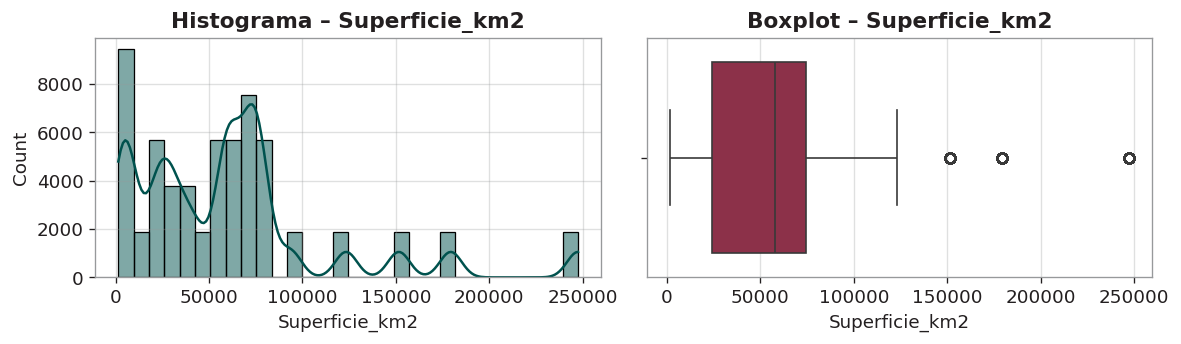
\includegraphics[width=\textwidth]{img/eda_hist_numericas.png}
    \caption{Histogramas de variables numéricas (superficie, ratio H/M, densidad poblacional).}
\end{figure}

\begin{figure}[H]
    \centering
    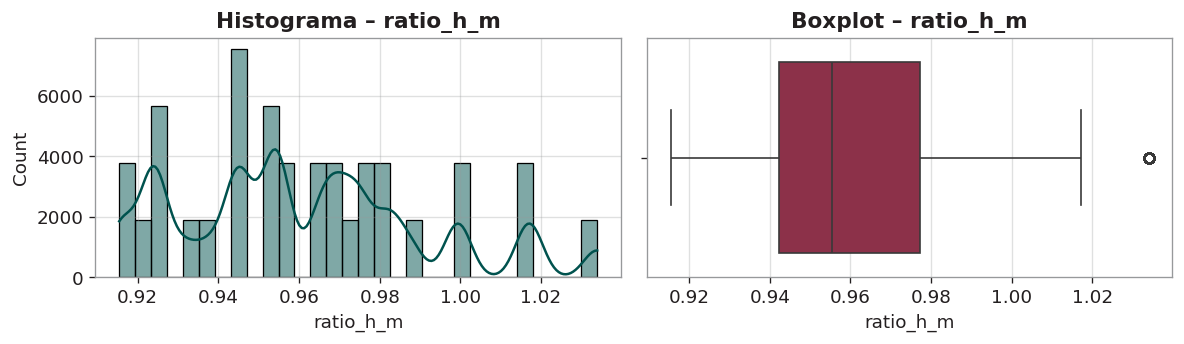
\includegraphics[width=\textwidth]{img/eda_boxplot_numericas.png}
    \caption{Boxplots de variables numéricas.}
\end{figure}

\begin{figure}[H]
    \centering
    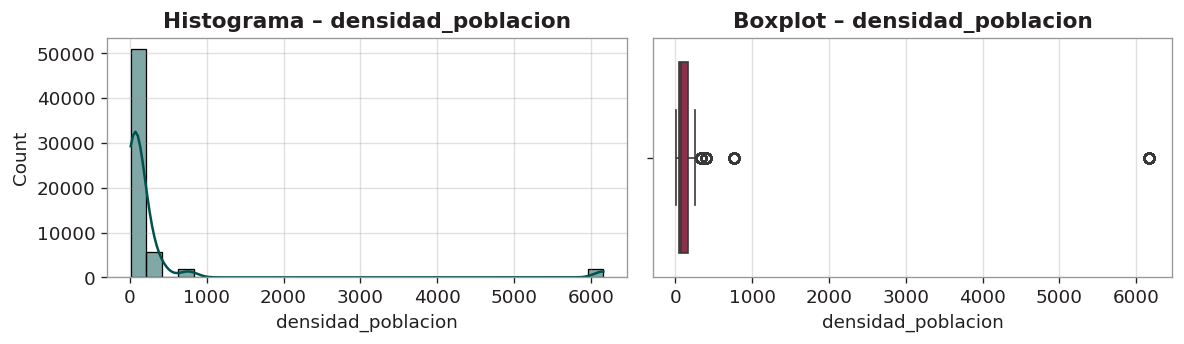
\includegraphics[width=\textwidth]{img/eda_barras_categoricas.png}
    \caption{Distribución de variables categóricas (región, tamaño poblacional, ratio H/M categorizado).}
\end{figure}

\begin{figure}[H]
    \centering
    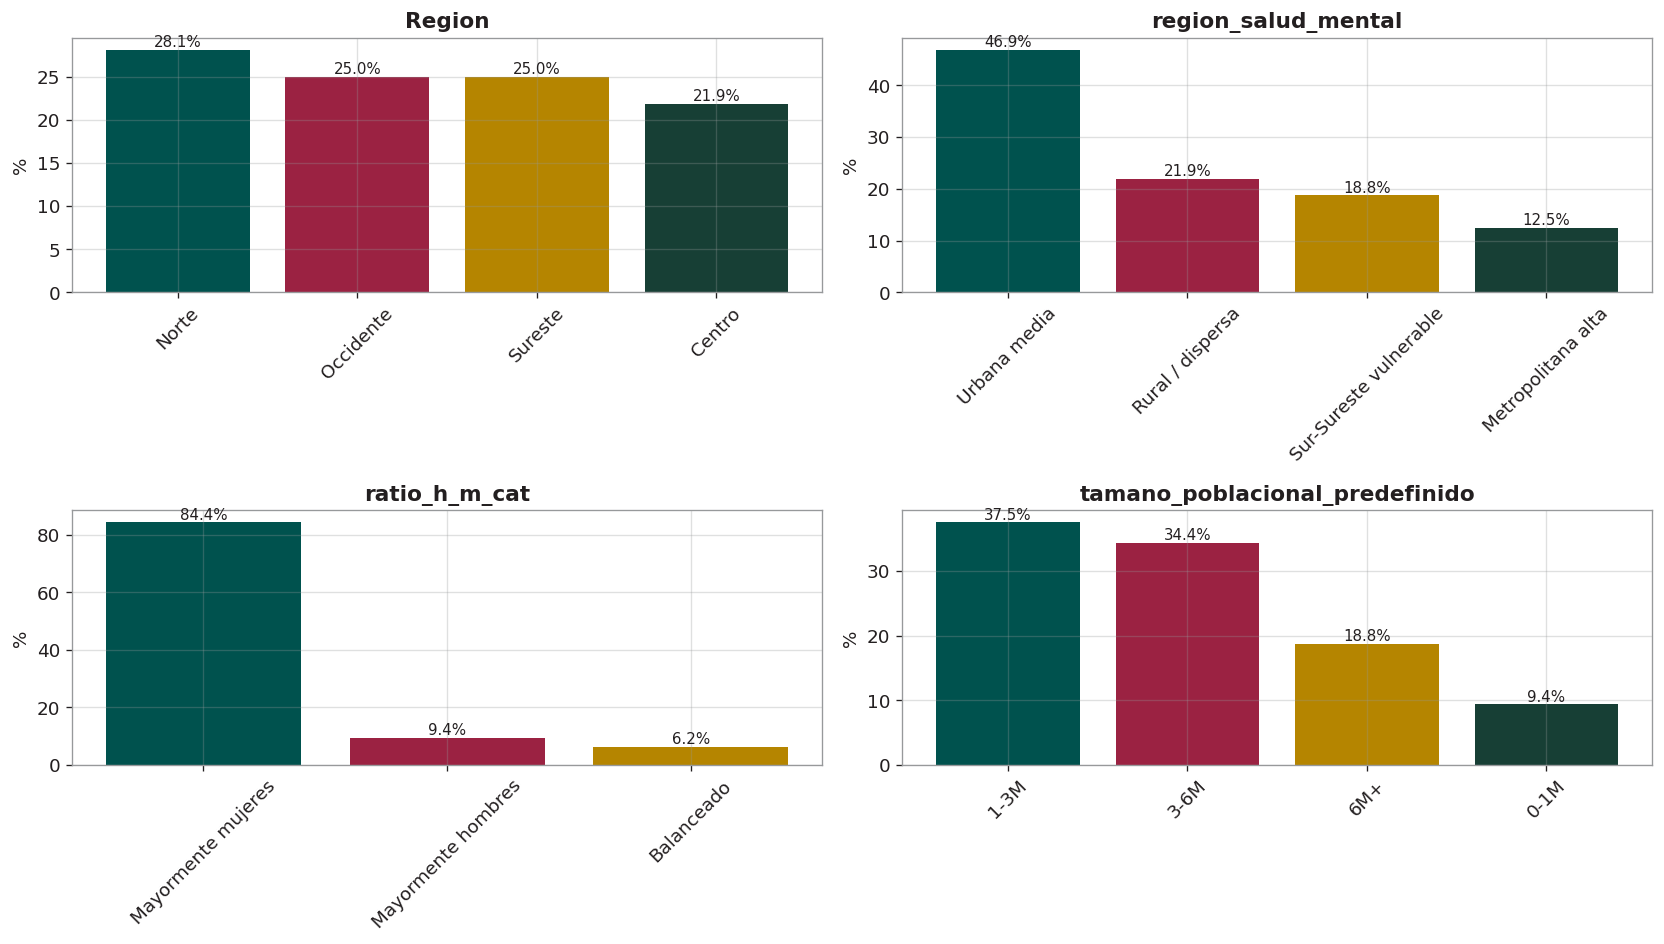
\includegraphics[width=\textwidth]{img/eda_heatmap_correlacion.png}
    \caption{Mapa de calor de correlaciones entre variables numéricas.}
\end{figure}

\subsection{Interpretación rápida de las visualizaciones estructurales}

\subsubsection{Variables numéricas}

\paragraph{Superficie territorial (\code{Superficie\_km2}).}
La distribución de la superficie territorial muestra una asimetría positiva marcada, con varios outliers naturales asociados a estados de gran extensión territorial (Chihuahua, Sonora, Coahuila). Este comportamiento justifica el uso posterior de percentiles o categorizaciones, ya que el uso directo de la variable puede dominar análisis multivariados.

\paragraph{Densidad poblacional (\code{densidad\_poblacion}).}
La densidad poblacional presenta una asimetría extrema, con un outlier dominante claramente identificado: la Ciudad de México (entidad con superficie muy pequeña y población muy alta). Este resultado confirma que la densidad poblacional es una variable altamente informativa en epidemiología, pero su uso directo sin transformación puede introducir sesgos fuertes.

\paragraph{Ratio hombres/mujeres (\code{ratio\_h\_m}).}
El ratio hombres/mujeres muestra una distribución compacta, centrada alrededor de 1, lo que indica que las entidades federativas presentan composiciones por sexo relativamente similares. No se observan valores extremos relevantes.

\subsubsection{Variables categóricas}

\paragraph{Clasificación hombres/mujeres (\code{ratio\_h\_m\_cat}).}
La versión categórica del ratio revela una limitación importante de diseño: la categoría ``Mayormente mujeres'' concentra más del 84\% de las entidades, lo que indica que la categorización actual no discrimina adecuadamente y podría requerir umbrales más estrictos.

\paragraph{Regiones territoriales.}
Ambas clasificaciones (\code{Region} y \code{region\_salud\_mental}) muestran distribuciones razonablemente balanceadas, sin concentraciones extremas. Son candidatas adecuadas para análisis estratificados y variables exógenas en modelos.

\paragraph{Tamaño poblacional (\code{tamano\_poblacional\_\allowbreak predefinido}).}
La categorización por rangos fijos de población muestra una distribución gradual entre grupos, reflejando la heterogeneidad demográfica del país. Esta variable conserva significado absoluto, lo que la hace más interpretable en términos de política pública.

\subsubsection{Conclusión exploratoria}

Las visualizaciones confirman que: las asimetrías territoriales y demográficas son estructurales (no errores); algunas variables categóricas (como \code{ratio\_h\_m\_cat}) requieren revisión metodológica; otras (región, tamaño poblacional) están bien definidas y aportan contexto valioso. Este análisis visual funciona como un \textit{sanity check} previo al modelado.

\newpage

% ============================================================
% SECCIÓN 7
% ============================================================
\section{Series de tiempo por categoría territorial}

En esta sección se visualiza la evolución temporal de los \textbf{incrementos semanales de casos}, diferenciados por categorías territoriales derivadas de INEGI. El objetivo es analizar la \textbf{dinámica epidemiológica a lo largo del tiempo}, incorporando un contexto estructural que permita comparar patrones entre distintos tipos de regiones.

% -------------------------------------------------------
\subsection{Región de salud mental (\code{region\_salud\_mental})}

\textbf{Tipo:} Categórica nominal.
\textbf{Fuente:} Clasificación definida en el proyecto, apoyada en criterios socio-urbanos.

Esta categoría se asigna mediante un mapeo explícito entidad $\rightarrow$ región. Las regiones son: Metropolitana alta, Urbana media, Transición y Rural-dispersa.

\subsubsection*{Segregado por género}

\begin{figure}[H]
    \centering
    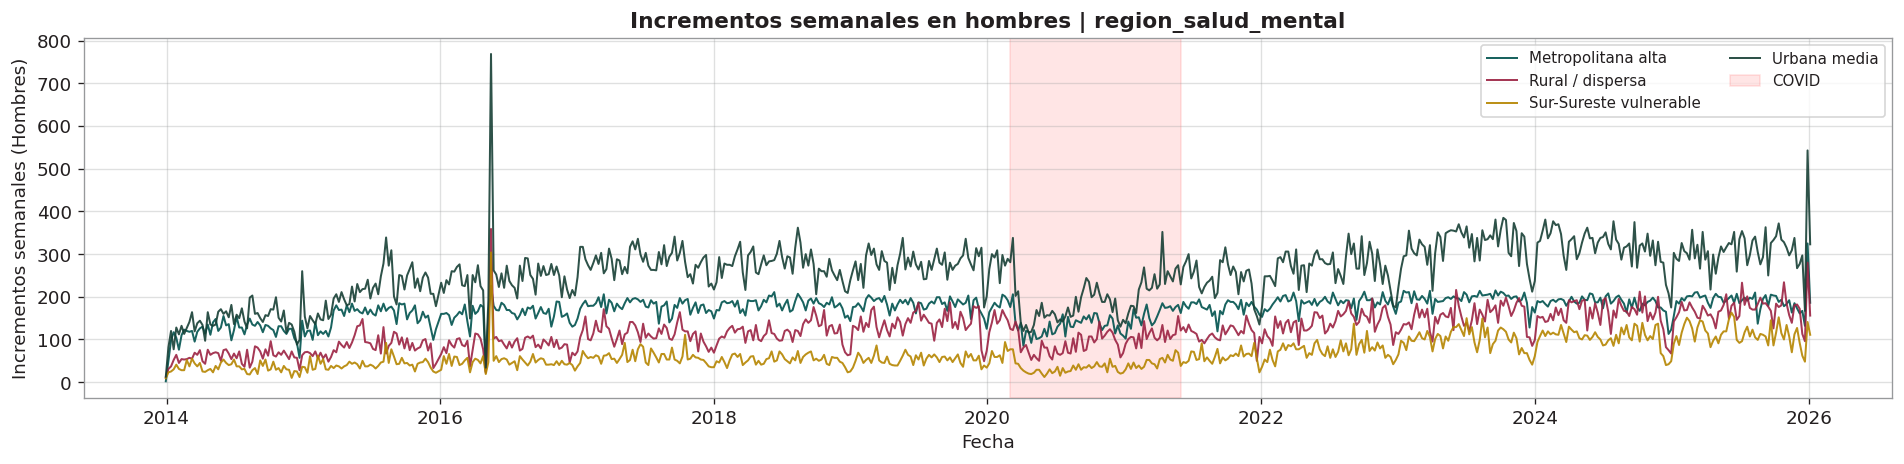
\includegraphics[width=\textwidth]{img/st_region_salud_mental_genero_hombres.png}
    \caption{Región de salud mental -- Incrementos semanales (Hombres).}
\end{figure}

\begin{figure}[H]
    \centering
    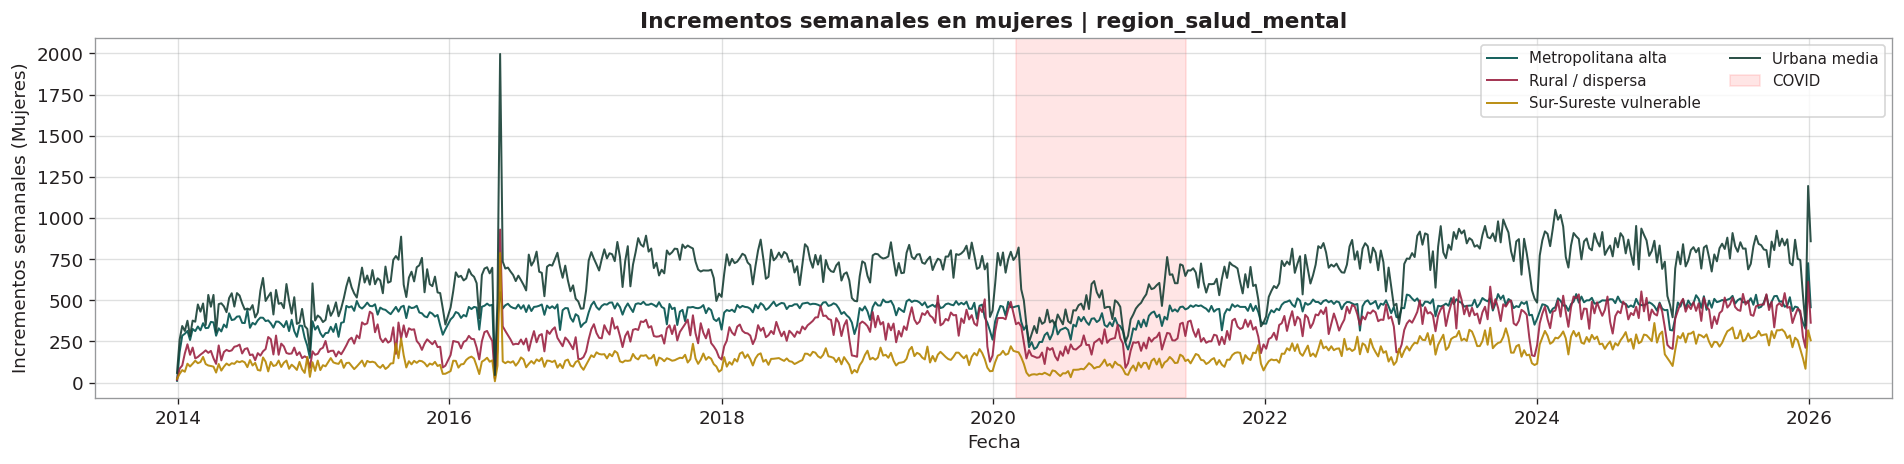
\includegraphics[width=\textwidth]{img/st_region_salud_mental_genero_mujeres.png}
    \caption{Región de salud mental -- Incrementos semanales (Mujeres).}
\end{figure}

\subsubsection*{Incrementos totales}

\begin{figure}[H]
    \centering
    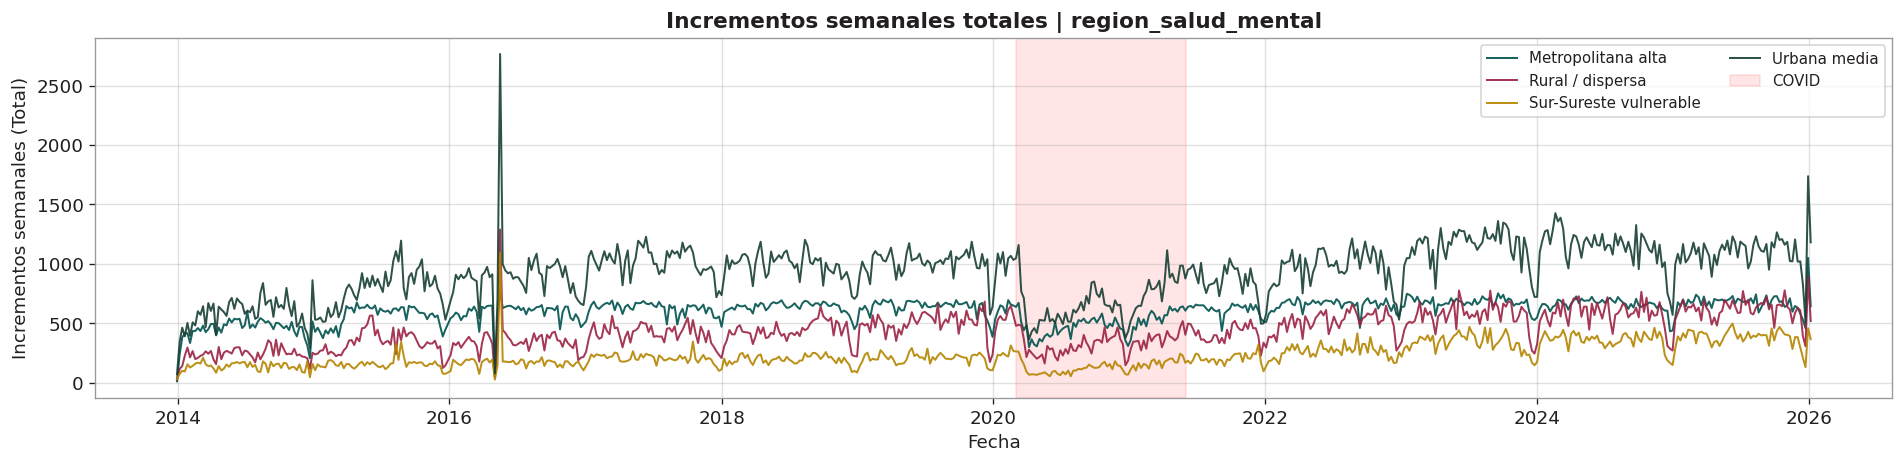
\includegraphics[width=\textwidth]{img/st_region_salud_mental_total.png}
    \caption{Región de salud mental -- Incrementos semanales totales.}
\end{figure}

% -------------------------------------------------------
\subsection{Densidad poblacional por percentiles (\code{densidad\_poblacional\_\allowbreak percentil})}

\textbf{Tipo:} Categórica ordinal.
\textbf{Fuente:} Variable derivada de población y superficie territorial (INEGI, 2020).

La densidad poblacional continua se discretiza en cuartiles. Las categorías son: Baja, Media-baja, Media-alta y Alta.

\subsubsection*{Segregado por género}

\begin{figure}[H]
    \centering
    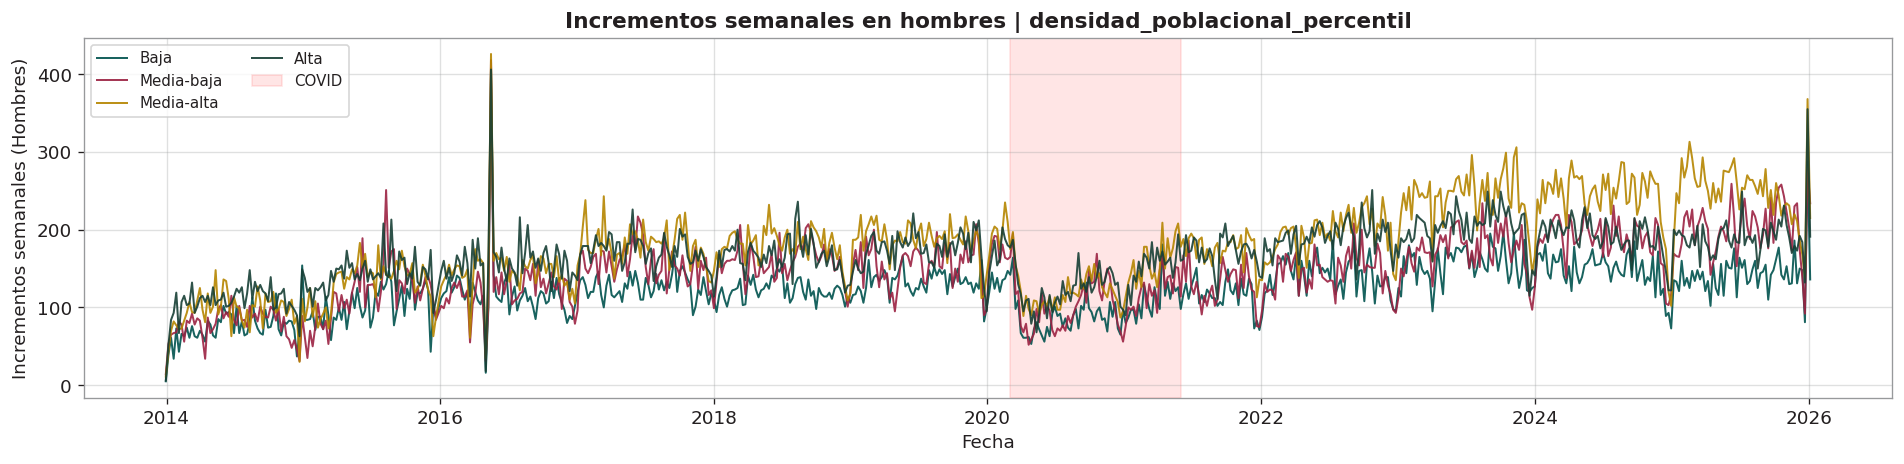
\includegraphics[width=\textwidth]{img/st_densidad_poblacional_genero_hombres.png}
    \caption{Densidad poblacional -- Incrementos semanales (Hombres).}
\end{figure}

\begin{figure}[H]
    \centering
    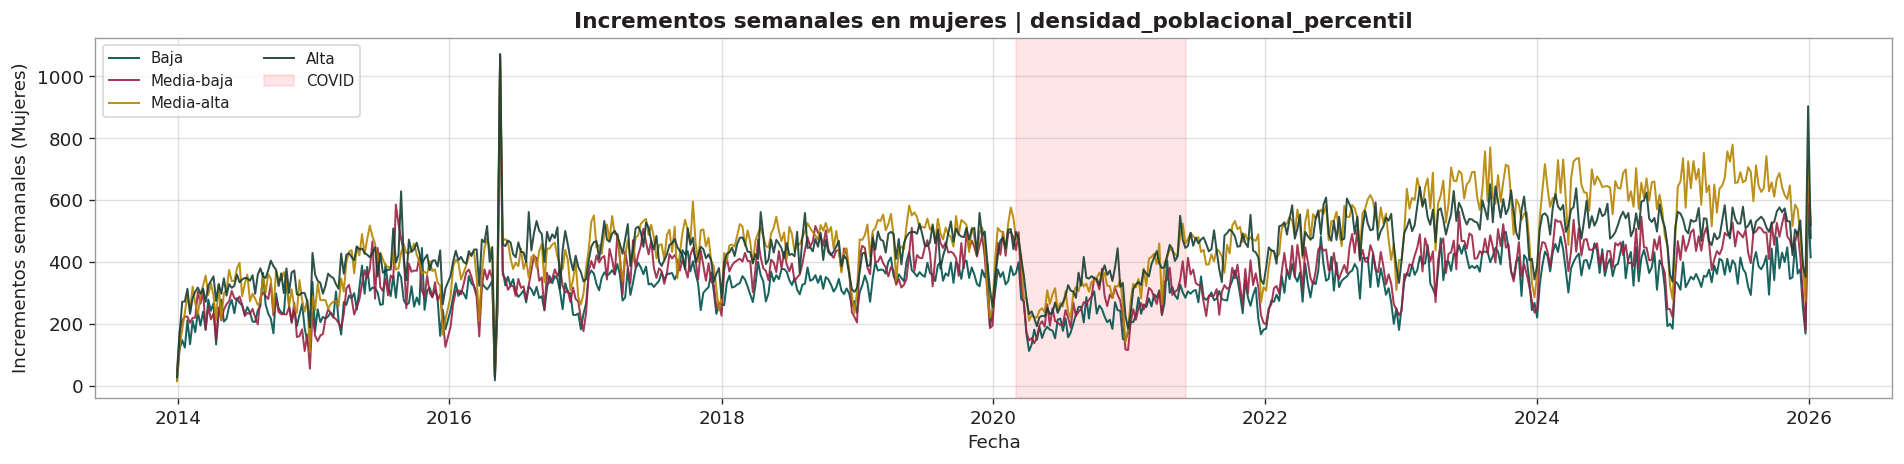
\includegraphics[width=\textwidth]{img/st_densidad_poblacional_genero_mujeres.png}
    \caption{Densidad poblacional -- Incrementos semanales (Mujeres).}
\end{figure}

\subsubsection*{Incrementos totales}

\begin{figure}[H]
    \centering
    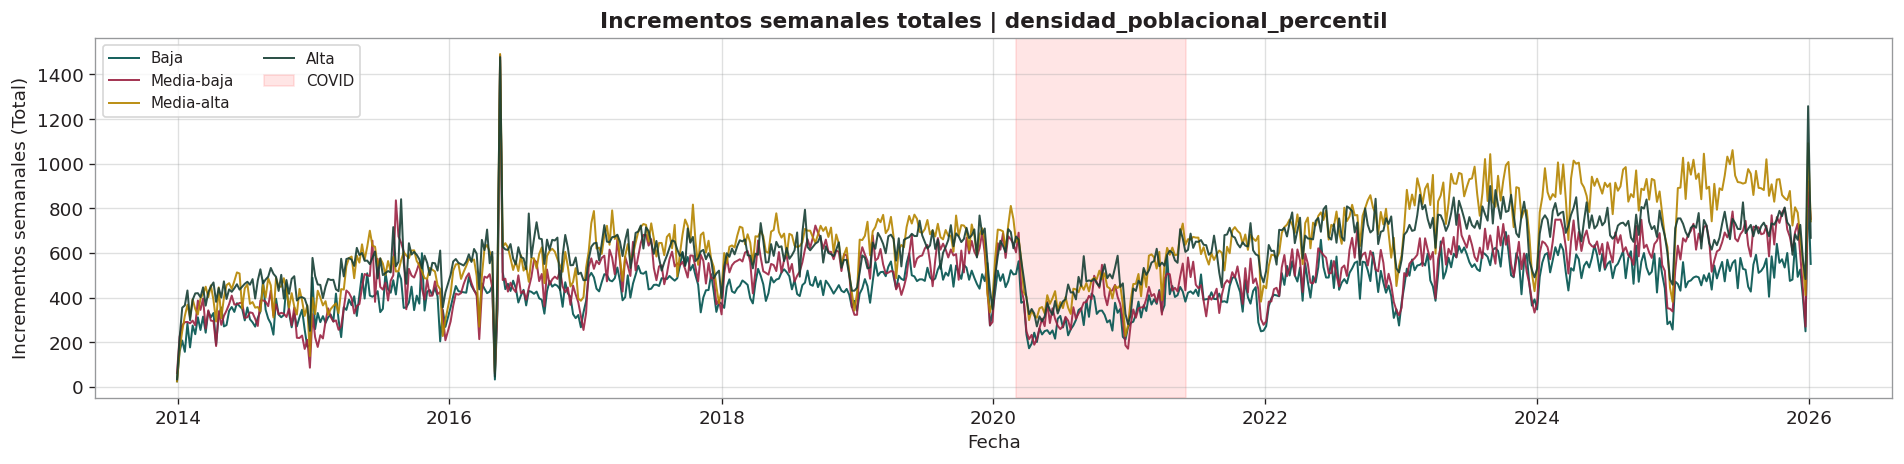
\includegraphics[width=\textwidth]{img/st_densidad_poblacional_total.png}
    \caption{Densidad poblacional -- Incrementos semanales totales.}
\end{figure}

% -------------------------------------------------------
\subsection{Tamaño poblacional por rangos fijos (\code{tamano\_poblacional\_\allowbreak predefinido})}

\textbf{Tipo:} Categórica ordinal.
\textbf{Fuente:} INEGI, población total (Censo 2020).

La población total se discretiza en rangos absolutos predefinidos: 0 a 1M, 1M a 3M, 3M a 6M y más de 6M habitantes.

\subsubsection*{Segregado por género}

\begin{figure}[H]
    \centering
    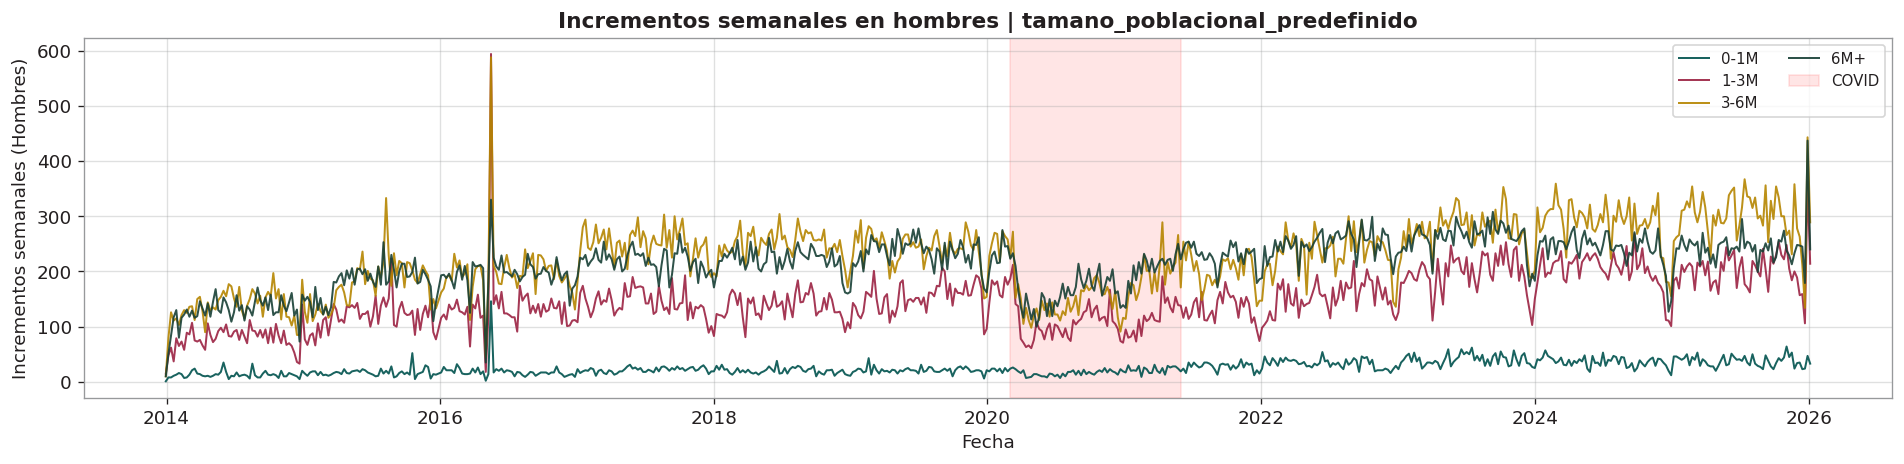
\includegraphics[width=\textwidth]{img/st_tamano_predefinido_genero_hombres.png}
    \caption{Tamaño poblacional (rangos fijos) -- Incrementos semanales (Hombres).}
\end{figure}

\begin{figure}[H]
    \centering
    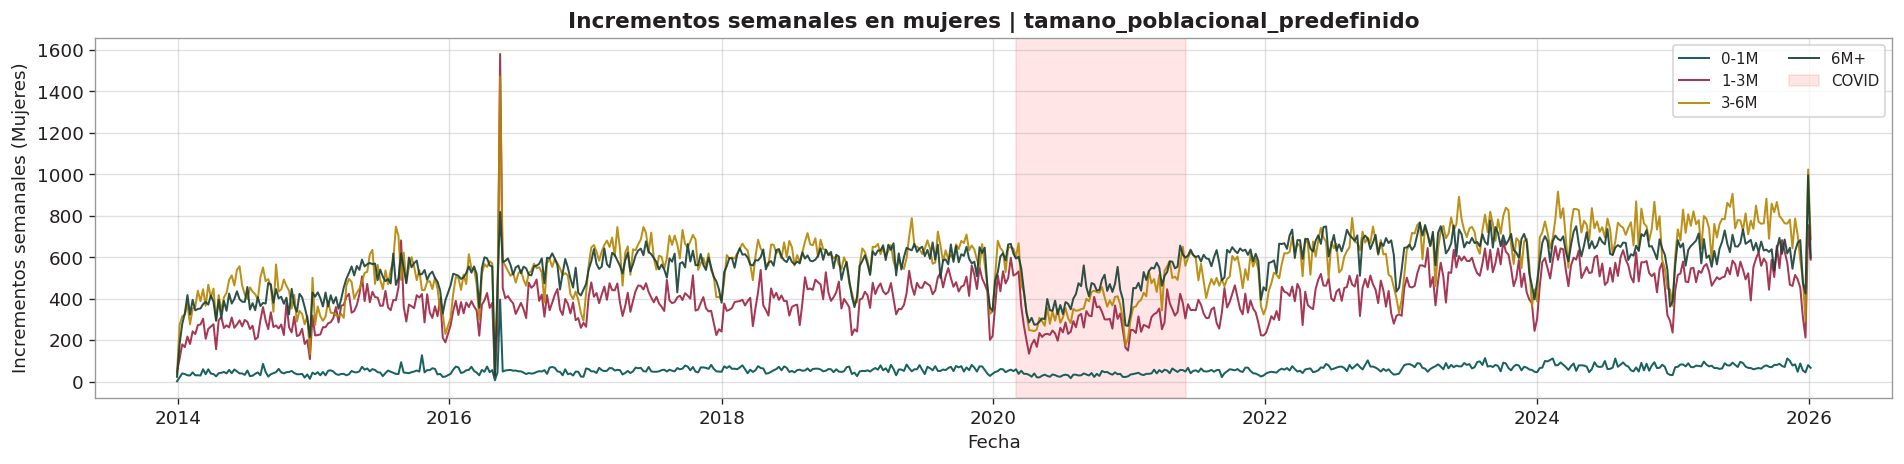
\includegraphics[width=\textwidth]{img/st_tamano_predefinido_genero_mujeres.png}
    \caption{Tamaño poblacional (rangos fijos) -- Incrementos semanales (Mujeres).}
\end{figure}

\subsubsection*{Incrementos totales}

\begin{figure}[H]
    \centering
    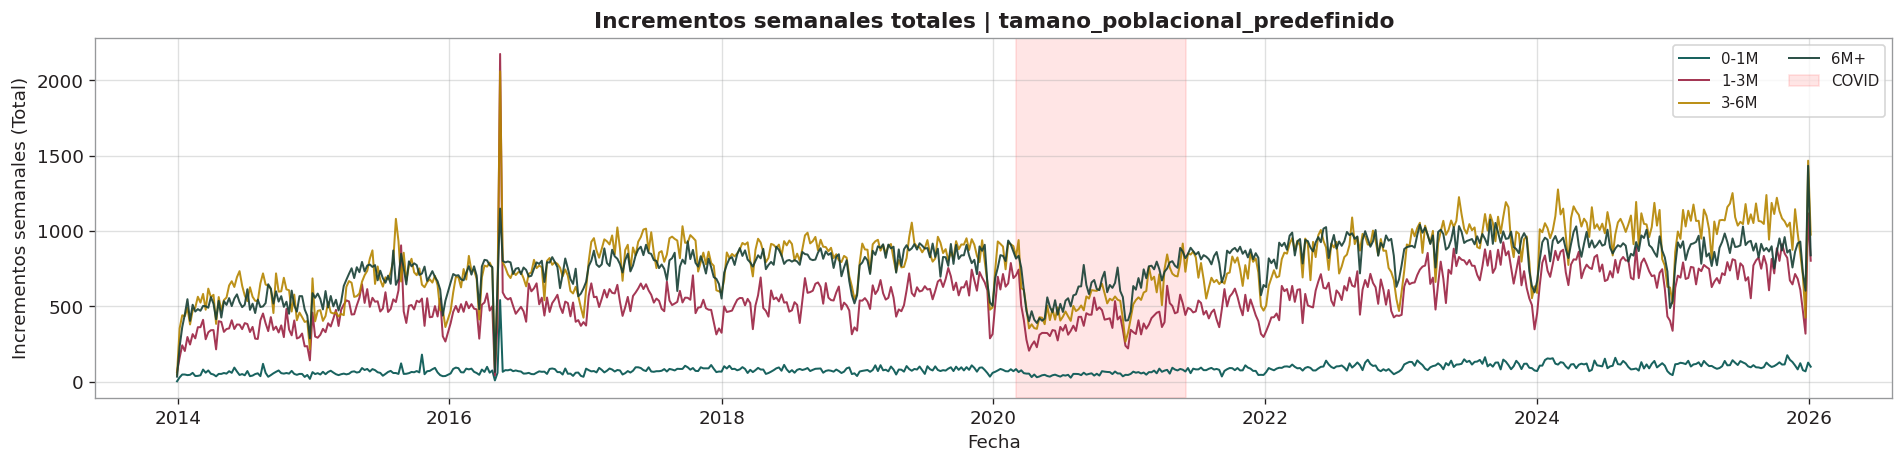
\includegraphics[width=\textwidth]{img/st_tamano_predefinido_total.png}
    \caption{Tamaño poblacional (rangos fijos) -- Incrementos semanales totales.}
\end{figure}

% -------------------------------------------------------
\subsection{Tamaño poblacional por percentiles (\code{tamano\_poblacional\_\allowbreak grupo\_percentil})}

\textbf{Tipo:} Categórica ordinal.
\textbf{Fuente:} INEGI, población total (Censo 2020).

La población total se agrupa mediante discretización por cuantiles, generando cuatro grupos de tamaño similar: Población baja, Media-baja, Media-alta y Alta.

\subsubsection*{Segregado por género}

\begin{figure}[H]
    \centering
    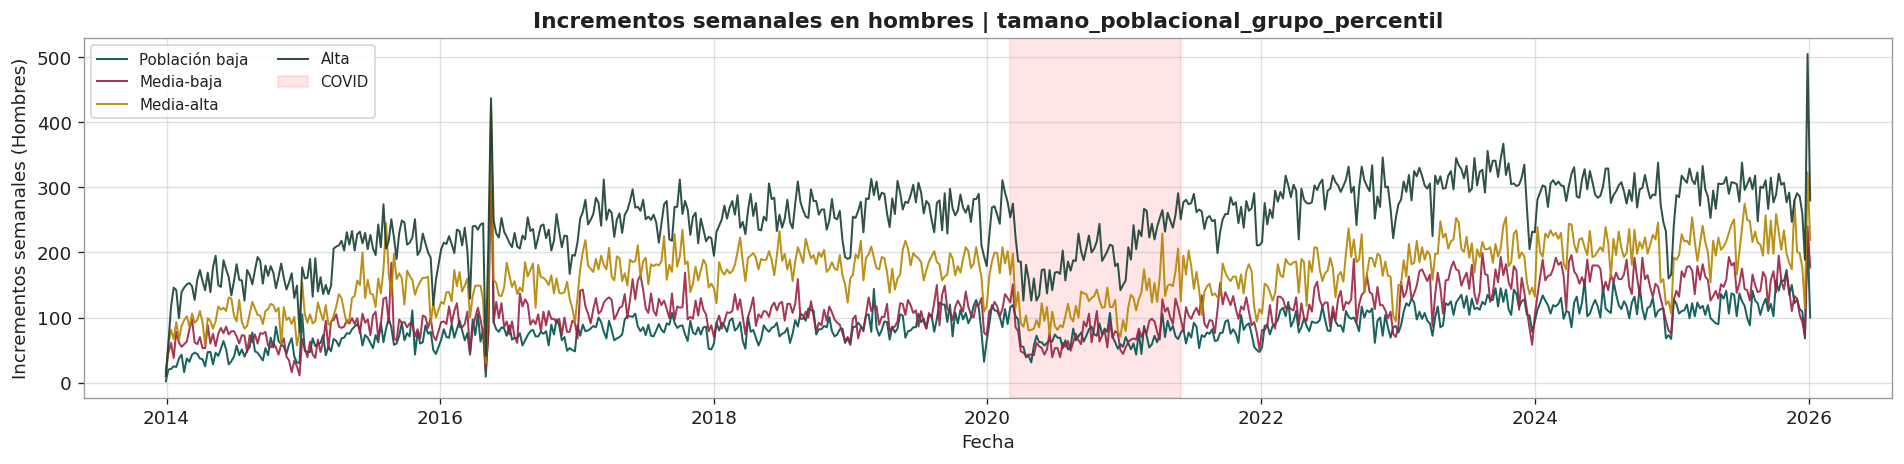
\includegraphics[width=\textwidth]{img/st_tamano_percentil_genero_hombres.png}
    \caption{Tamaño poblacional (percentiles) -- Incrementos semanales (Hombres).}
\end{figure}

\begin{figure}[H]
    \centering
    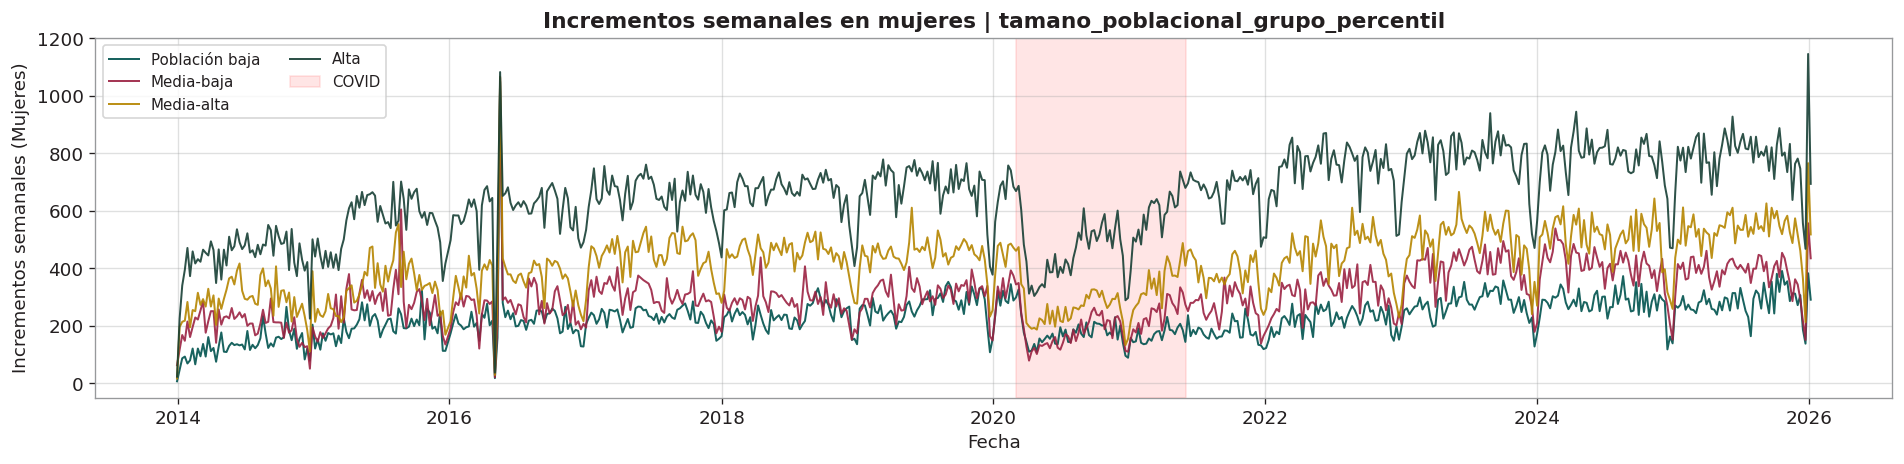
\includegraphics[width=\textwidth]{img/st_tamano_percentil_genero_mujeres.png}
    \caption{Tamaño poblacional (percentiles) -- Incrementos semanales (Mujeres).}
\end{figure}

\subsubsection*{Incrementos totales}

\begin{figure}[H]
    \centering
    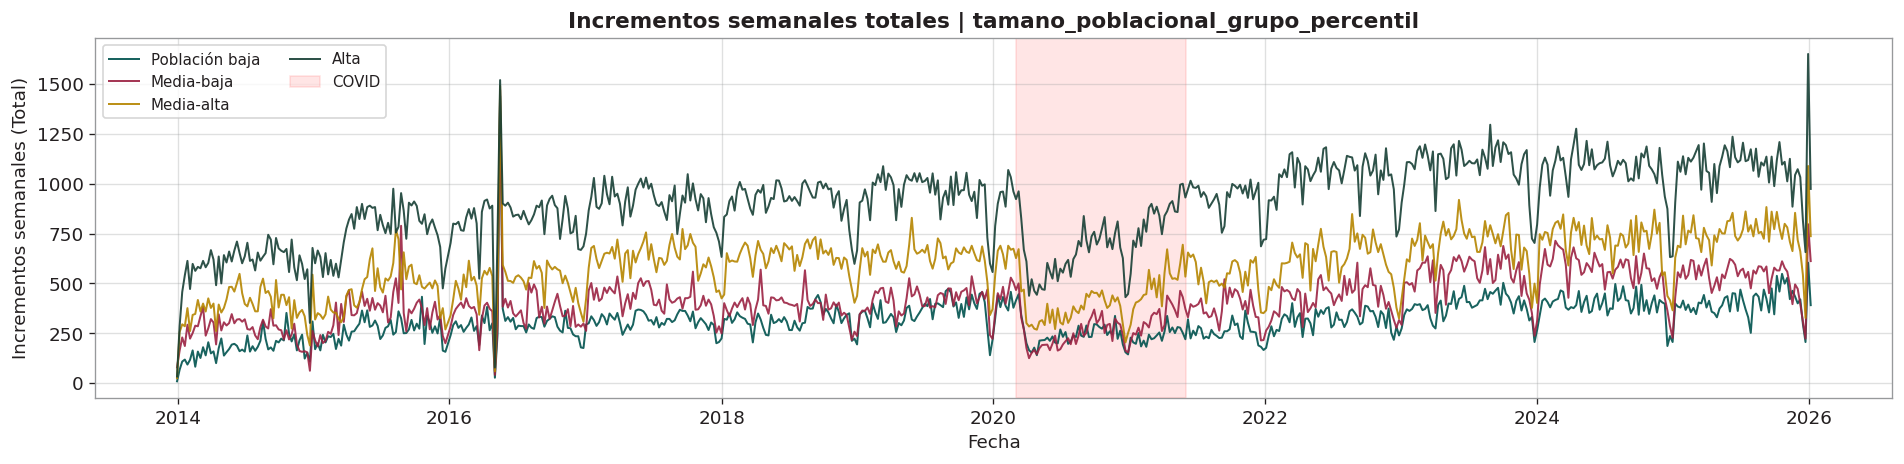
\includegraphics[width=\textwidth]{img/st_tamano_percentil_total.png}
    \caption{Tamaño poblacional (percentiles) -- Incrementos semanales totales.}
\end{figure}

% -------------------------------------------------------
\subsection{Extensión territorial por percentiles (\code{extension\_territorial\_\allowbreak percentil})}

\textbf{Tipo:} Categórica ordinal.
\textbf{Fuente:} INEGI, superficie territorial (km²).

La superficie territorial se discretiza en cuartiles: Territorio pequeño, Medio-pequeño, Medio-grande y Grande.

\subsubsection*{Segregado por género}

\begin{figure}[H]
    \centering
    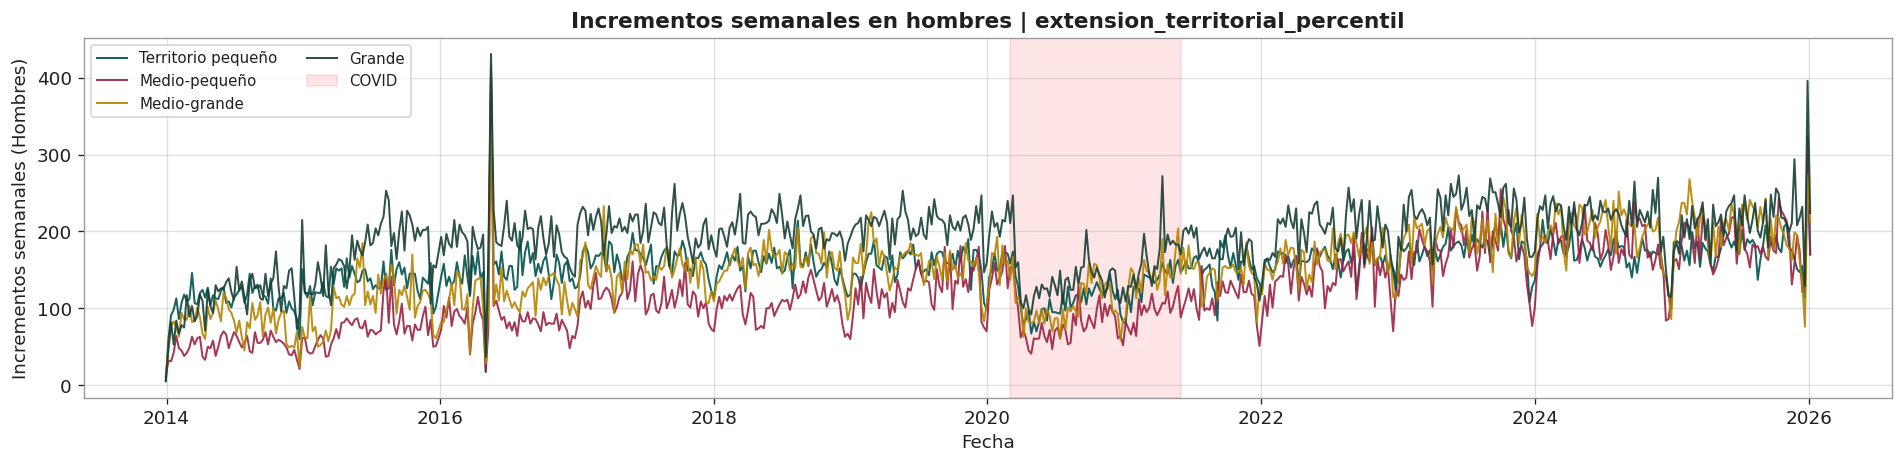
\includegraphics[width=\textwidth]{img/st_extension_territorial_genero_hombres.png}
    \caption{Extensión territorial -- Incrementos semanales (Hombres).}
\end{figure}

\begin{figure}[H]
    \centering
    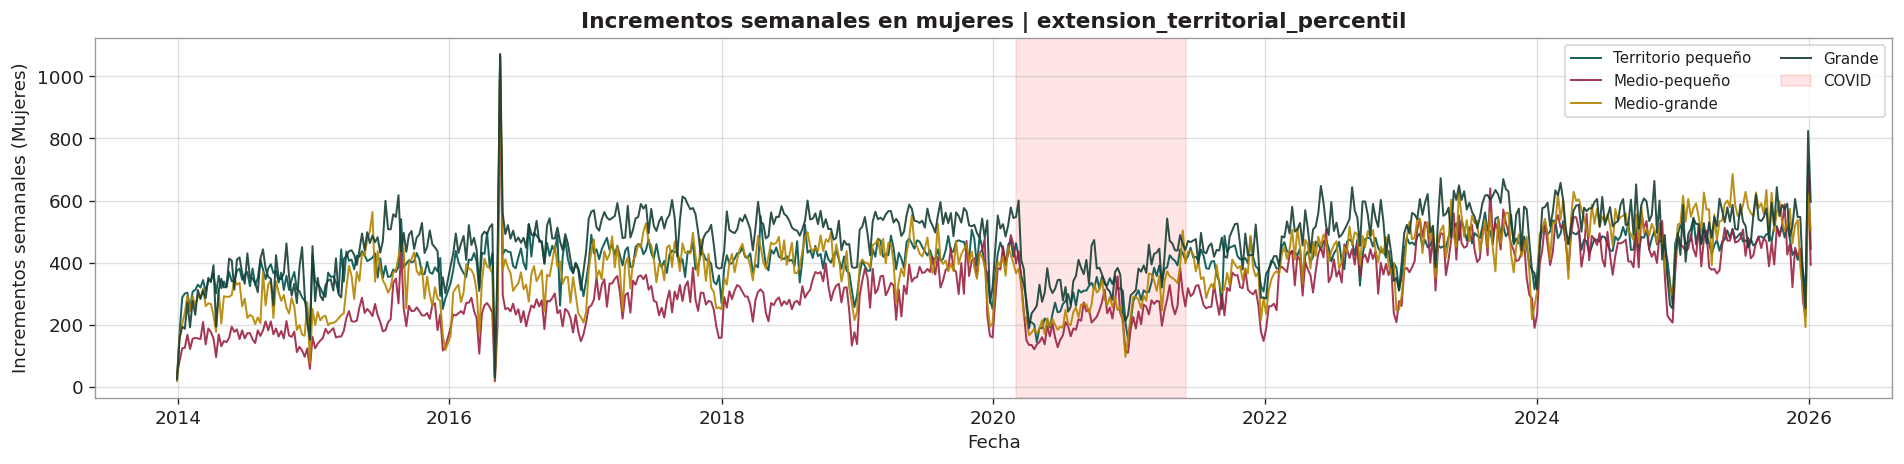
\includegraphics[width=\textwidth]{img/st_extension_territorial_genero_mujeres.png}
    \caption{Extensión territorial -- Incrementos semanales (Mujeres).}
\end{figure}

\subsubsection*{Incrementos totales}

\begin{figure}[H]
    \centering
    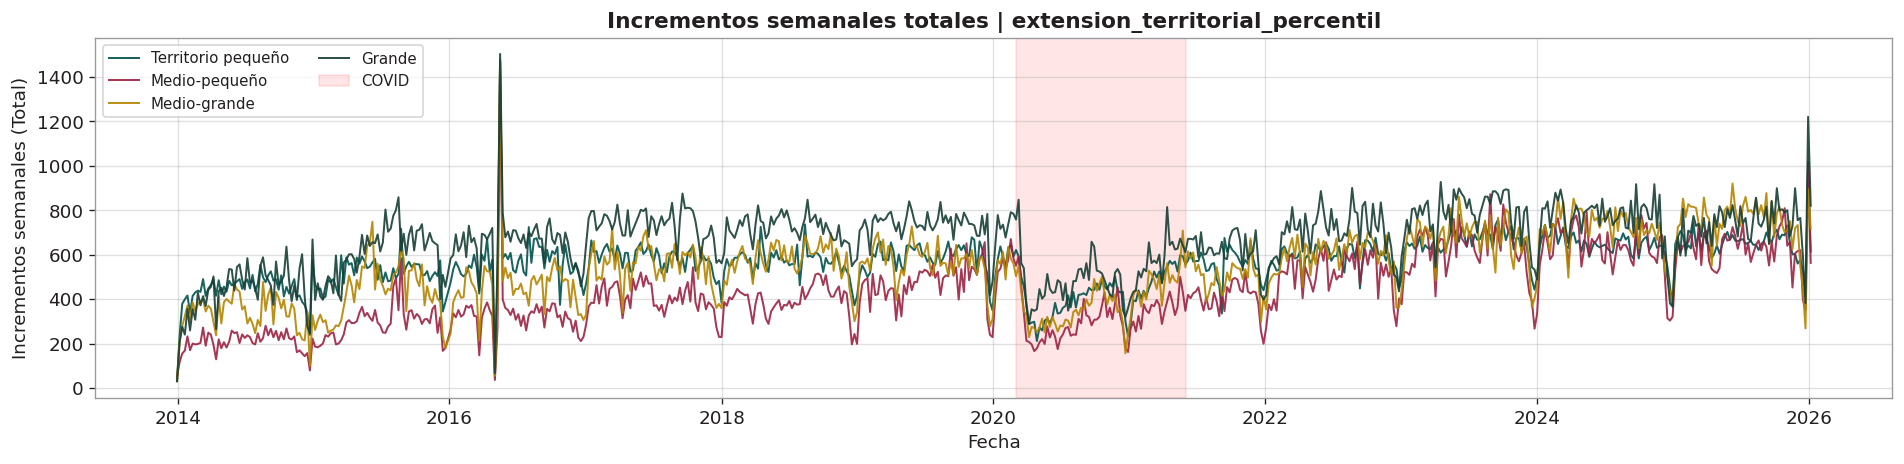
\includegraphics[width=\textwidth]{img/st_extension_territorial_total.png}
    \caption{Extensión territorial -- Incrementos semanales totales.}
\end{figure}

% -------------------------------------------------------
\subsection{Ratio hombres/mujeres categorizado (\code{ratio\_h\_m\_cat})}

\textbf{Tipo:} Categórica ordinal.
\textbf{Fuente:} INEGI, población por sexo (Censo 2020).

Se calcula el ratio continuo entre población masculina y femenina, y se discretiza: menor a 0.99 (Mayormente mujeres), entre 0.99 y 1.01 (Balanceado) y mayor a 1.01 (Mayormente hombres).

\subsubsection*{Segregado por género}

\begin{figure}[H]
    \centering
    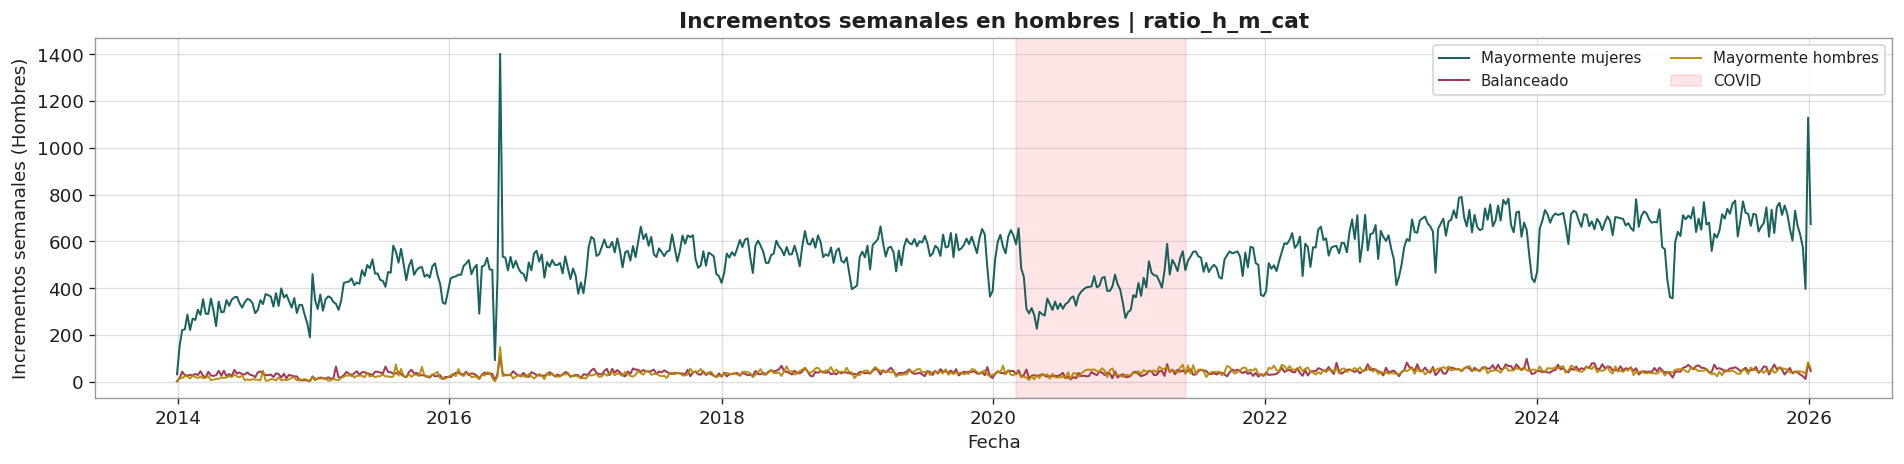
\includegraphics[width=\textwidth]{img/st_ratio_hm_genero_hombres.png}
    \caption{Ratio H/M -- Incrementos semanales (Hombres).}
\end{figure}

\begin{figure}[H]
    \centering
    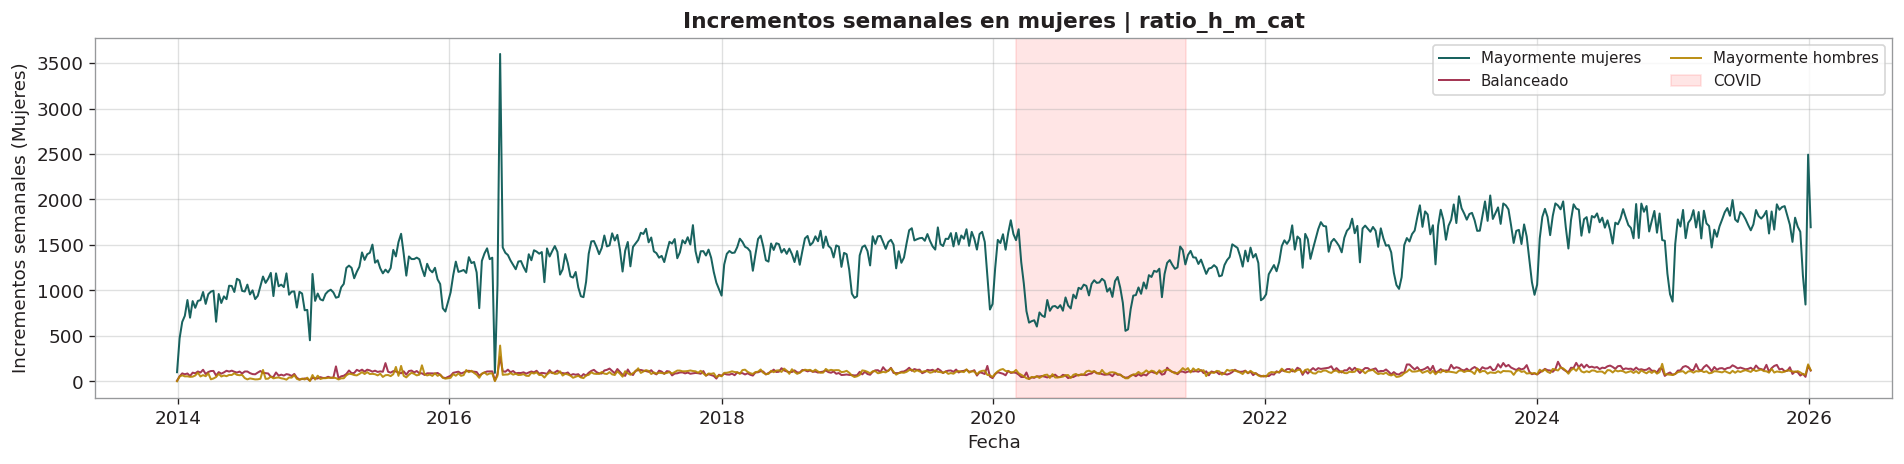
\includegraphics[width=\textwidth]{img/st_ratio_hm_genero_mujeres.png}
    \caption{Ratio H/M -- Incrementos semanales (Mujeres).}
\end{figure}

\subsubsection*{Incrementos totales}

\begin{figure}[H]
    \centering
    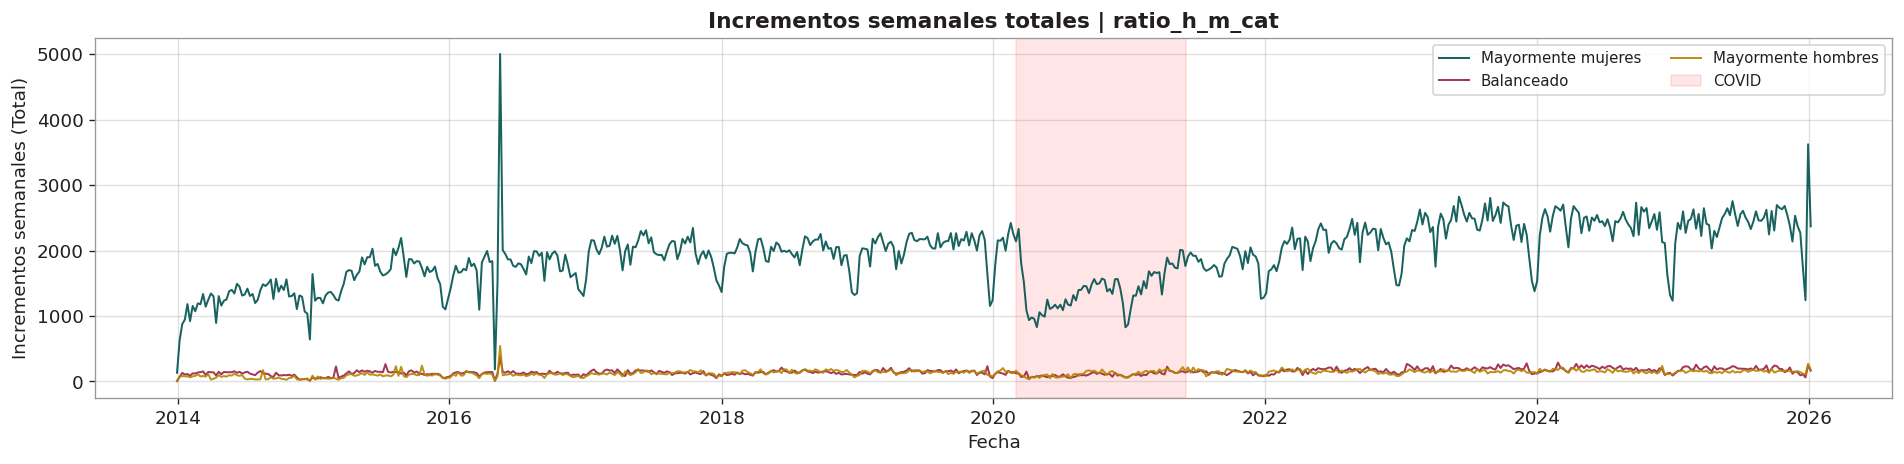
\includegraphics[width=\textwidth]{img/st_ratio_hm_total.png}
    \caption{Ratio H/M -- Incrementos semanales totales.}
\end{figure}

% ══════════════════════════════════════════════════════════════════════════════
% SECCIÓN 7.7 — ANÁLISIS POR ENTIDAD FEDERATIVA (VERSIÓN FINAL)
% Insertar DESPUÉS de subsección 7.6 (ratio_h_m) y ANTES de sección 8
% Imágenes van en la carpeta img/ de Overleaf
% ══════════════════════════════════════════════════════════════════════════════

\subsection{Análisis por entidad federativa}

Las secciones anteriores agruparon las entidades en categorías territoriales para analizar patrones epidemiológicos. En esta subsección se profundiza en el \textbf{comportamiento individual por estado}, identificando cuáles entidades concentran la mayor carga epidemiológica, cómo cambia el panorama al normalizar por población y qué estados presentan patrones temporales diferenciados.

% -------------------------------------------------------
\subsubsection{Ranking de entidades por carga absoluta de casos}

Se presentan las 10 entidades con mayor número de incrementos acumulados (2012--2025) para cada padecimiento, desagregados por sexo.

\begin{figure}[H]
    \centering
    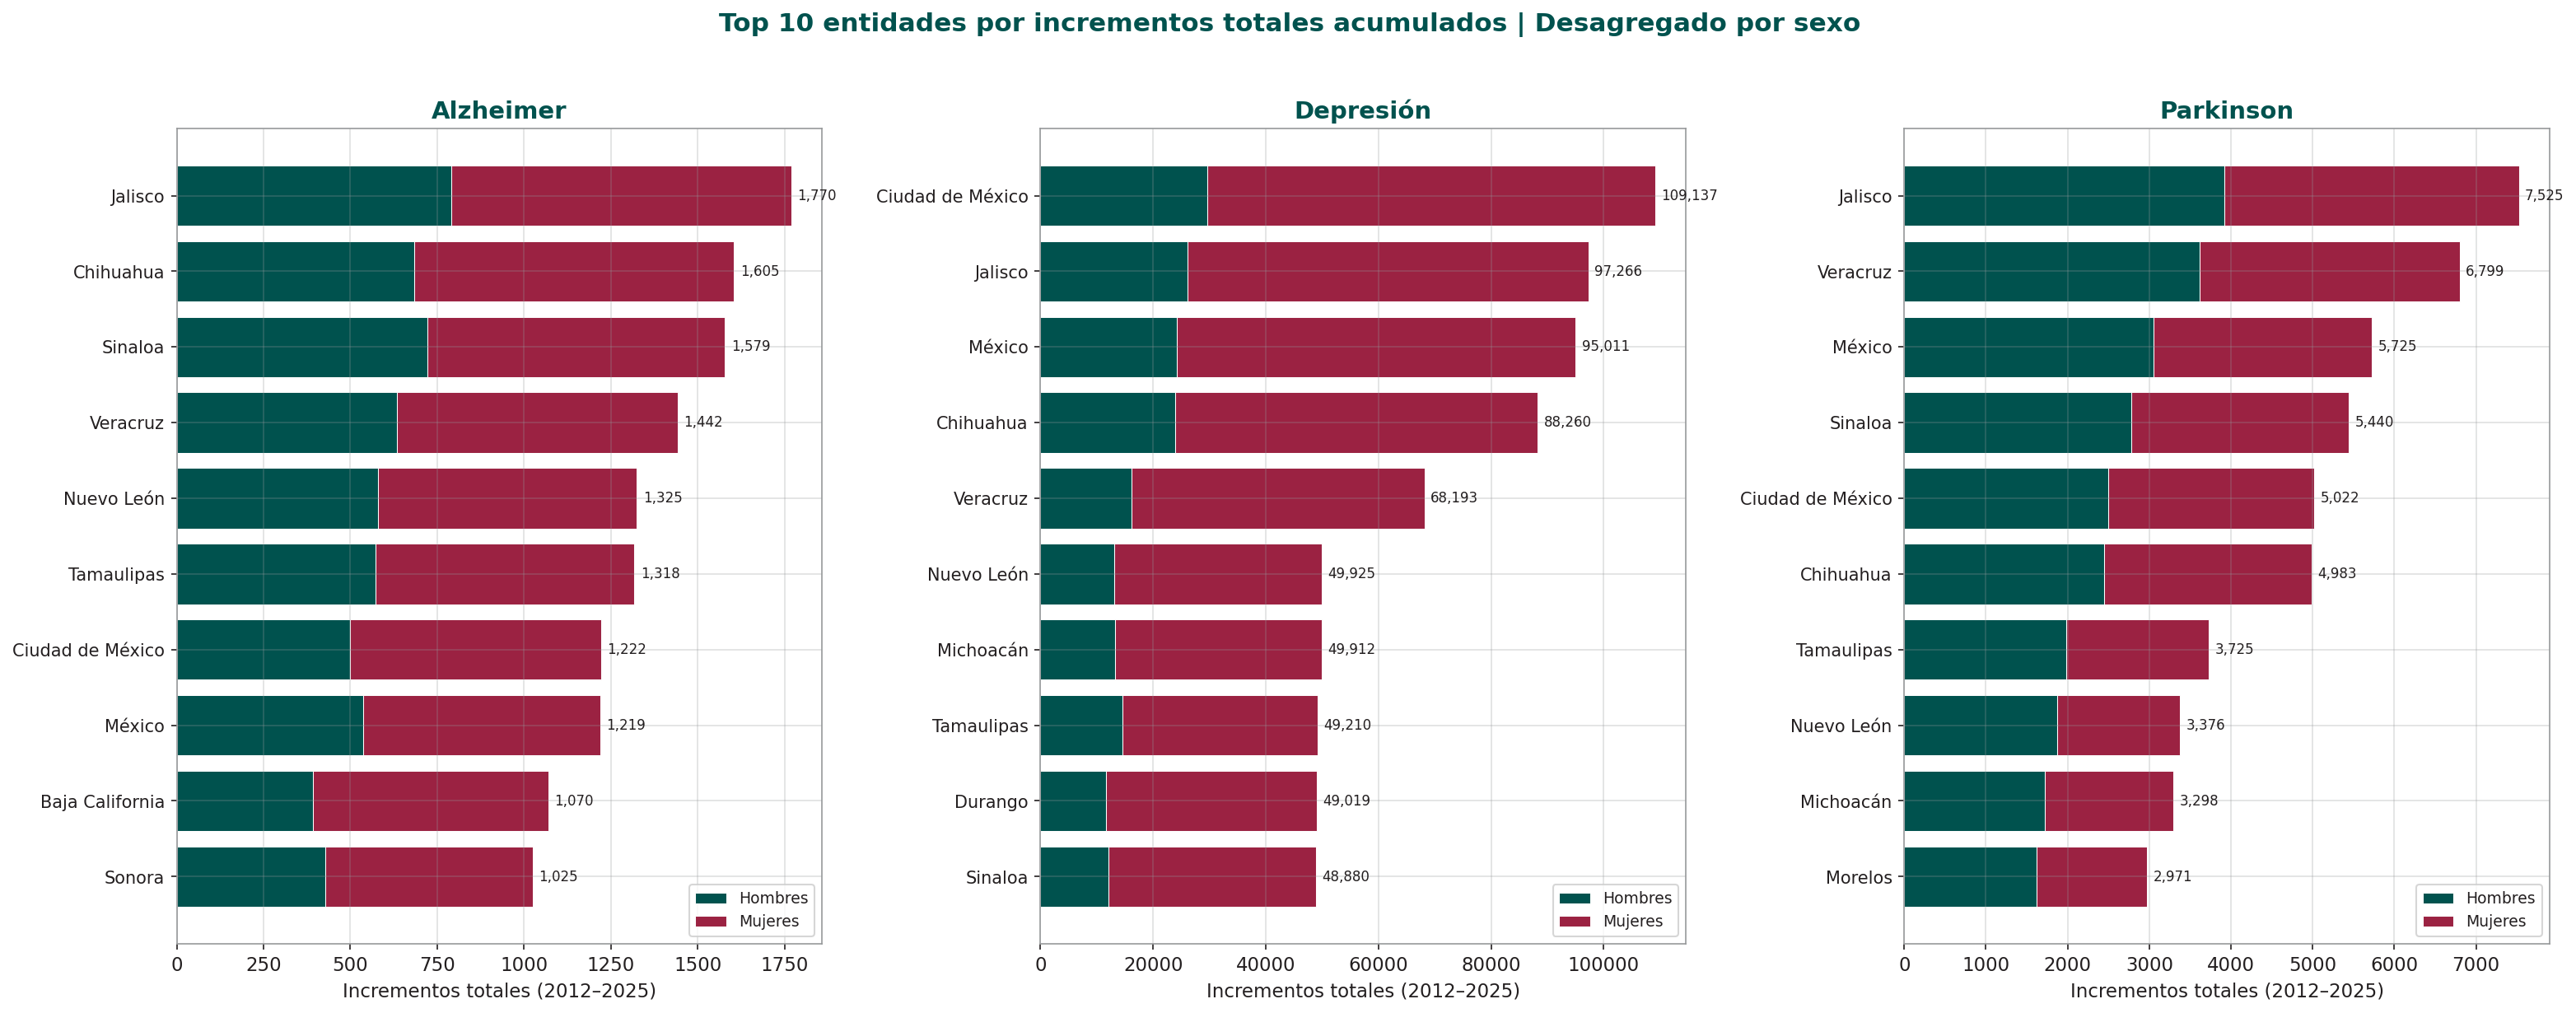
\includegraphics[width=\textwidth]{img/ranking_absoluto_entidades.png}
    \caption{Top 10 entidades por incrementos totales acumulados, desagregados por sexo.}
\end{figure}

% -------------------------------------------------------
\subsubsection{Ranking por tasa per cápita (por 100,000 habitantes)}

Al normalizar por población, el ranking cambia significativamente: entidades con menor población pero alta incidencia relativa emergen como prioritarias desde una perspectiva de salud pública.

\begin{figure}[H]
    \centering
    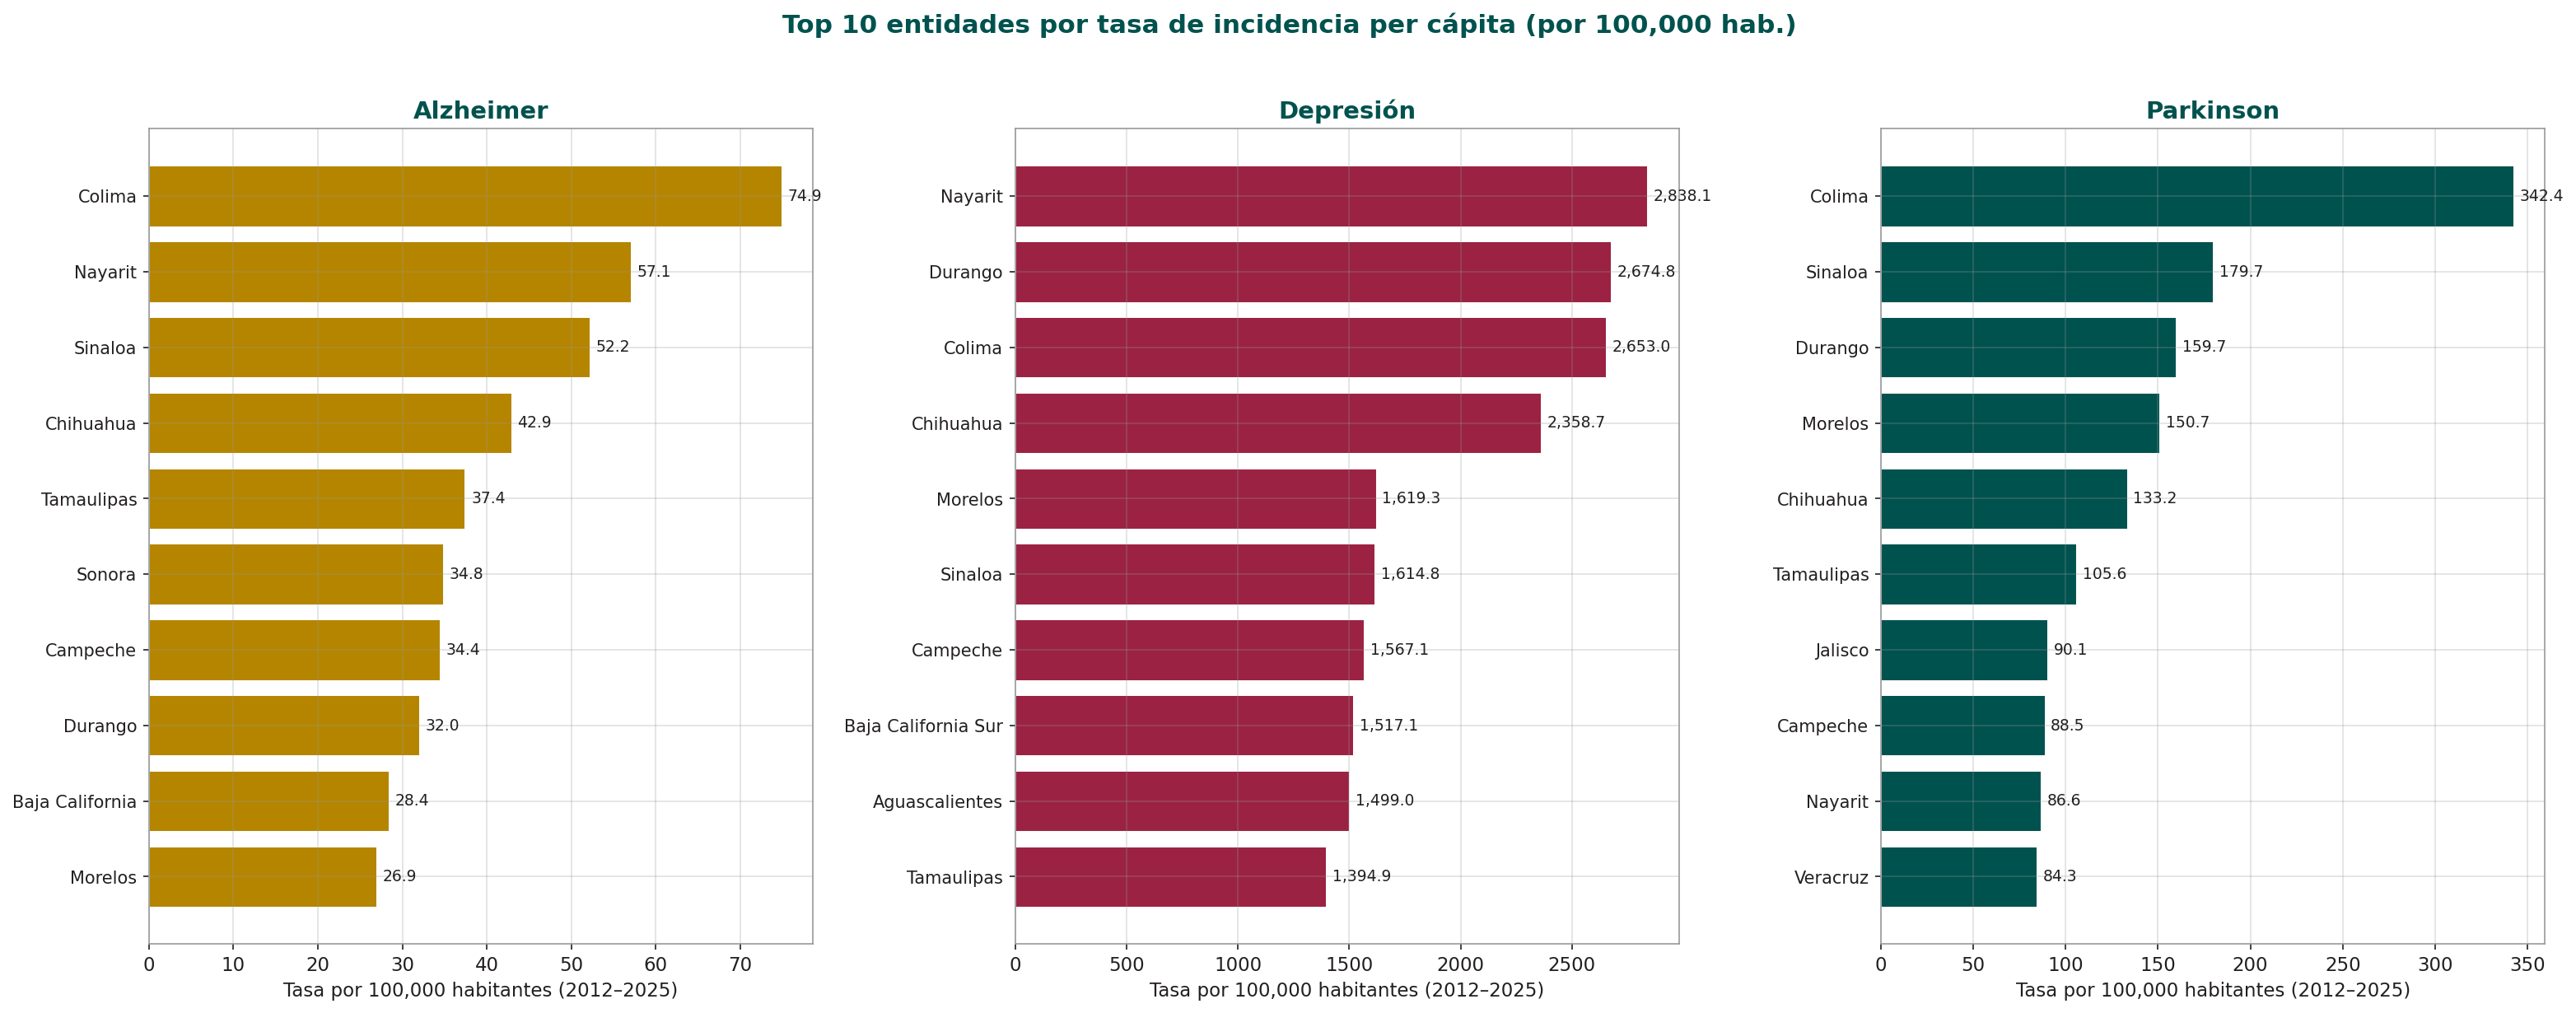
\includegraphics[width=\textwidth]{img/ranking_percapita_entidades.png}
    \caption{Top 10 entidades por tasa de incidencia per cápita (por 100,000 hab.).}
\end{figure}

% -------------------------------------------------------
\subsubsection{Heatmap: Incrementos anuales por entidad federativa}

El mapa de calor permite visualizar de manera simultánea todas las entidades a lo largo de todos los años, revelando patrones de concentración, brechas territoriales y el impacto diferenciado de la pandemia de COVID-19 por estado.

\begin{figure}[H]
    \centering
    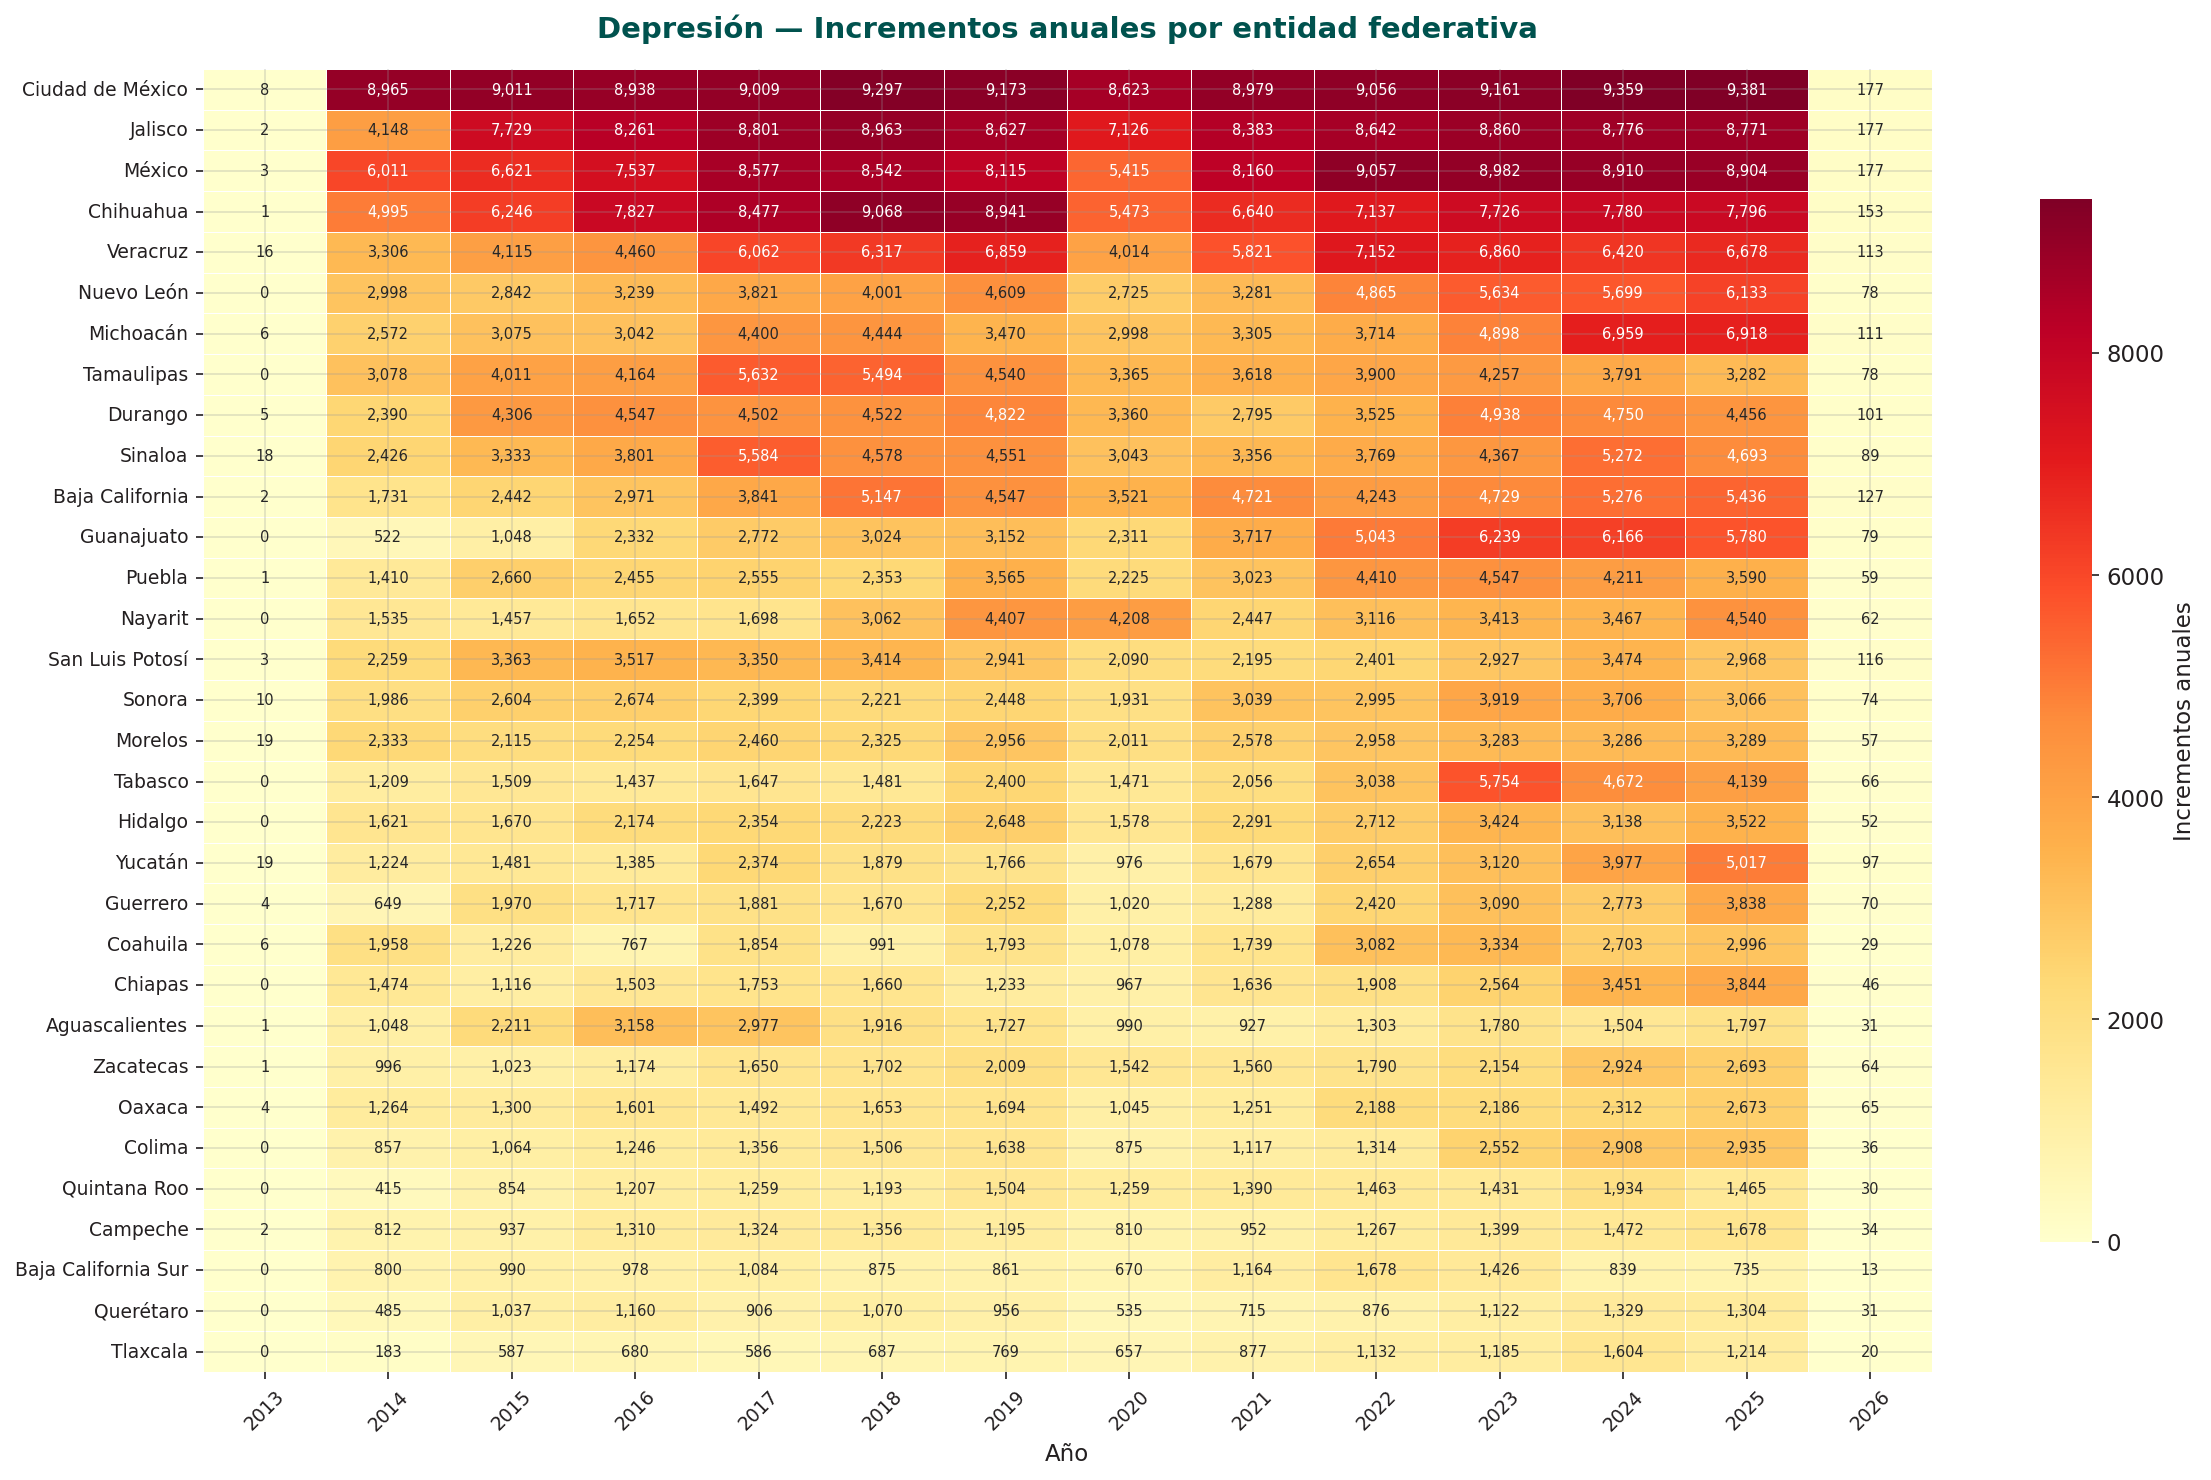
\includegraphics[width=\textwidth]{img/heatmap_entidad_anio_depresion.png}
    \caption{Depresión (F32) --- Incrementos anuales por entidad federativa.}
\end{figure}

\begin{figure}[H]
    \centering
    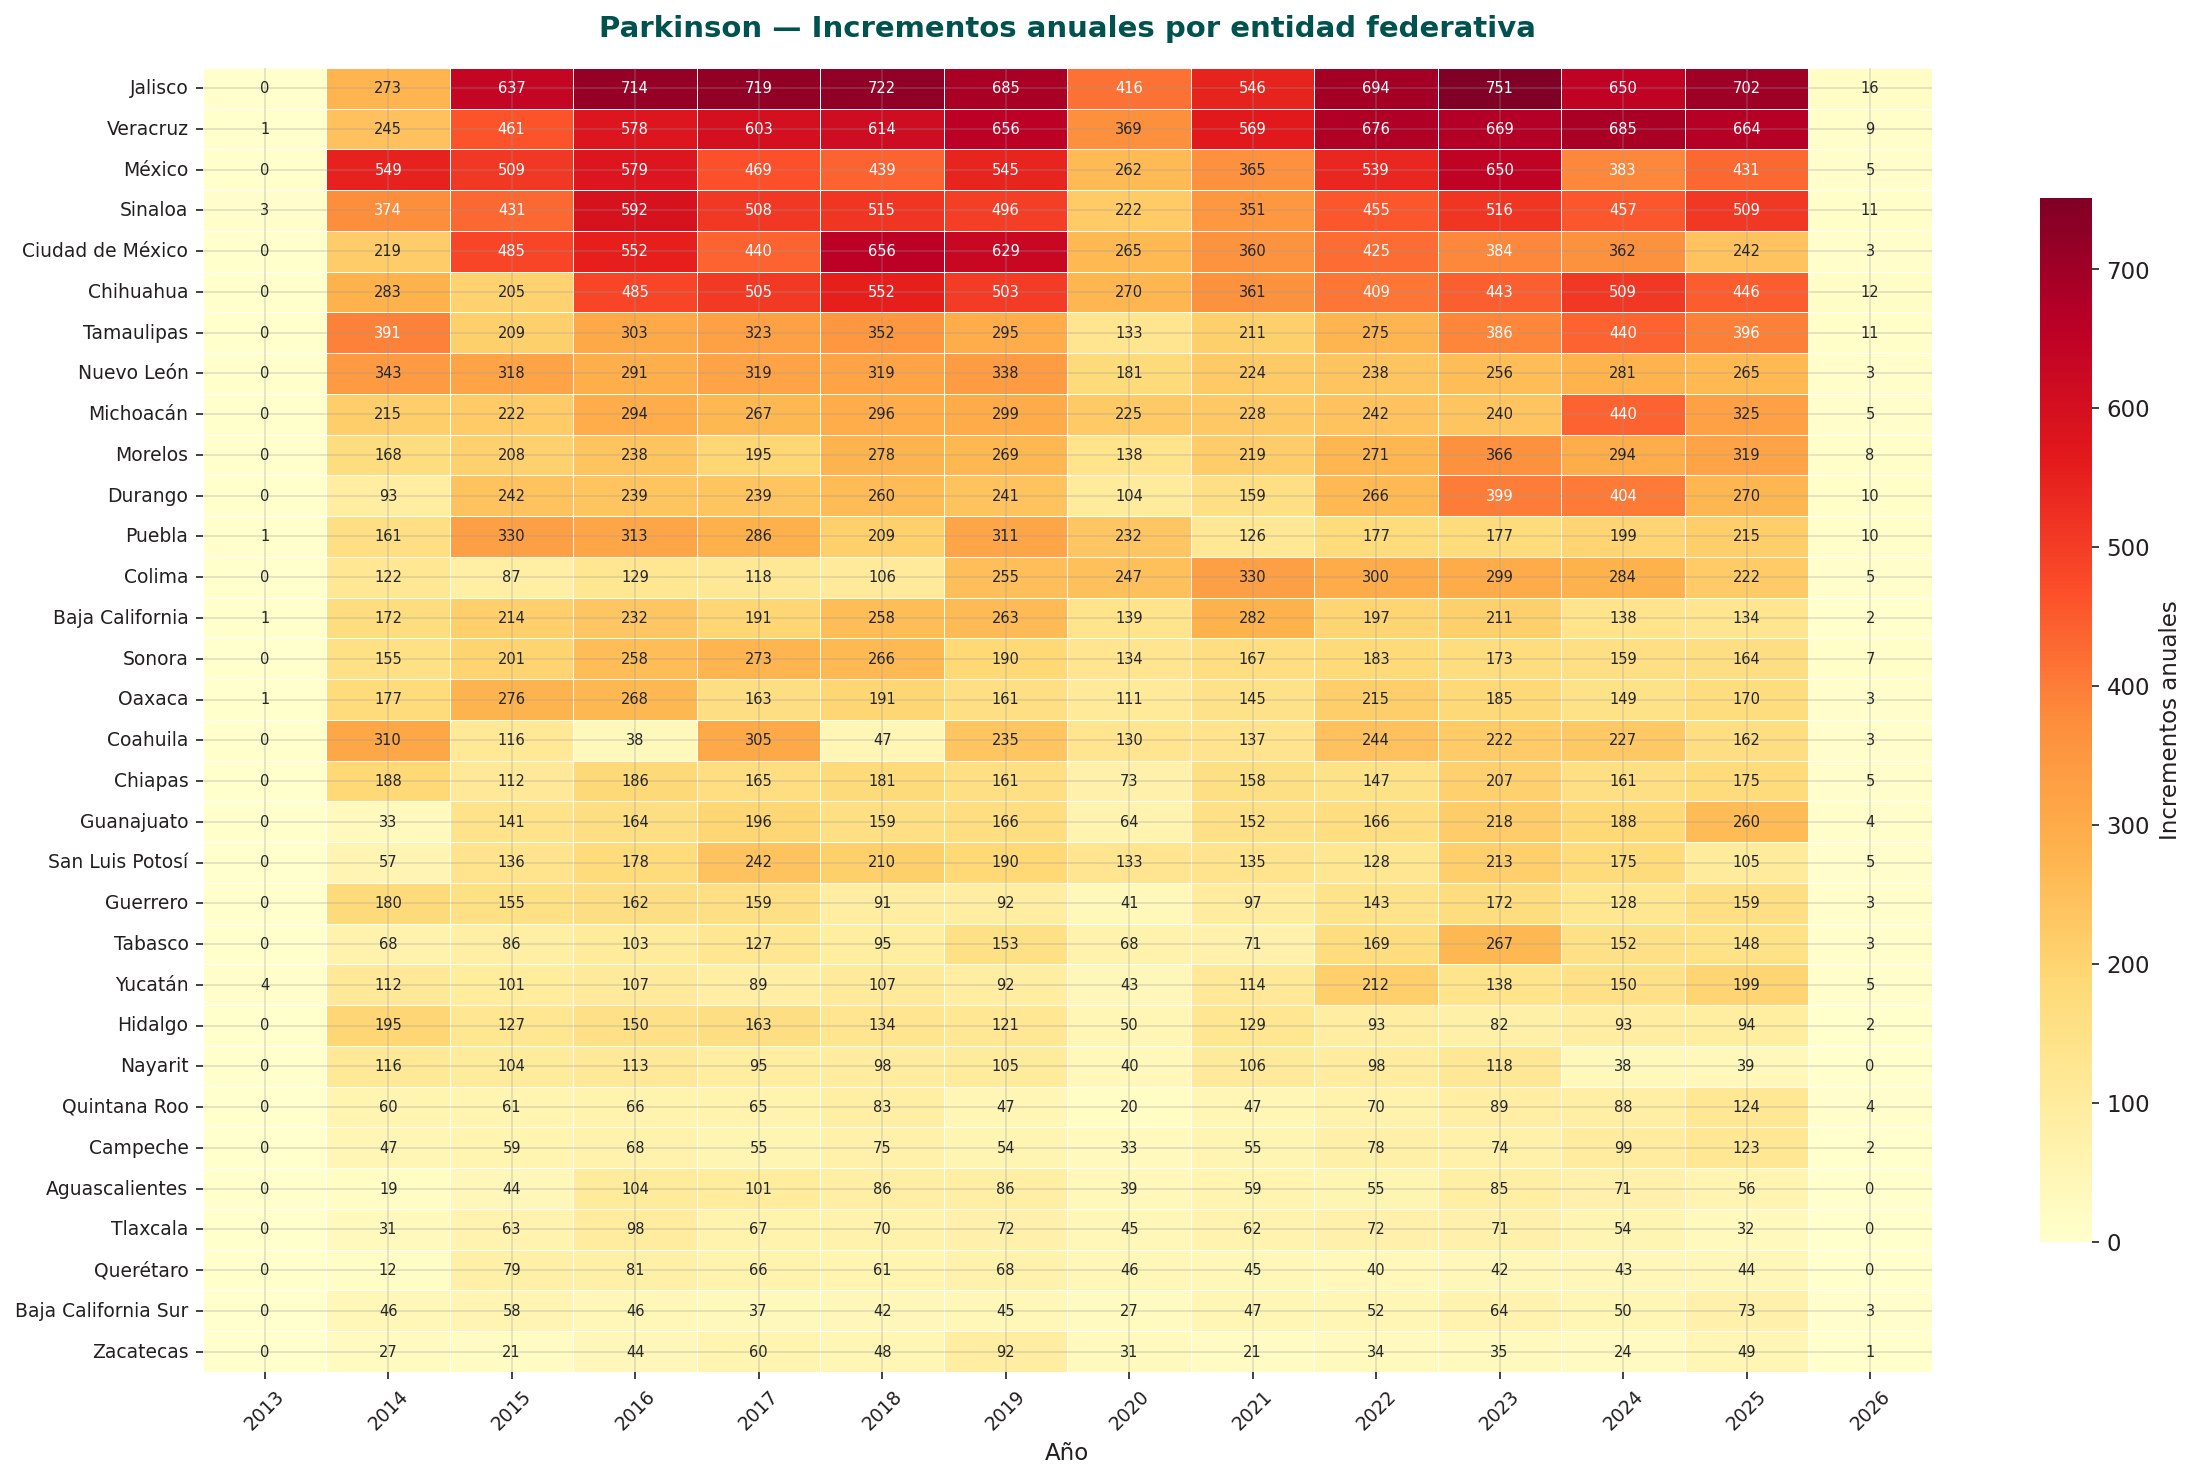
\includegraphics[width=\textwidth]{img/heatmap_entidad_anio_parkinson.png}
    \caption{Parkinson (G20) --- Incrementos anuales por entidad federativa.}
\end{figure}

\begin{figure}[H]
    \centering
    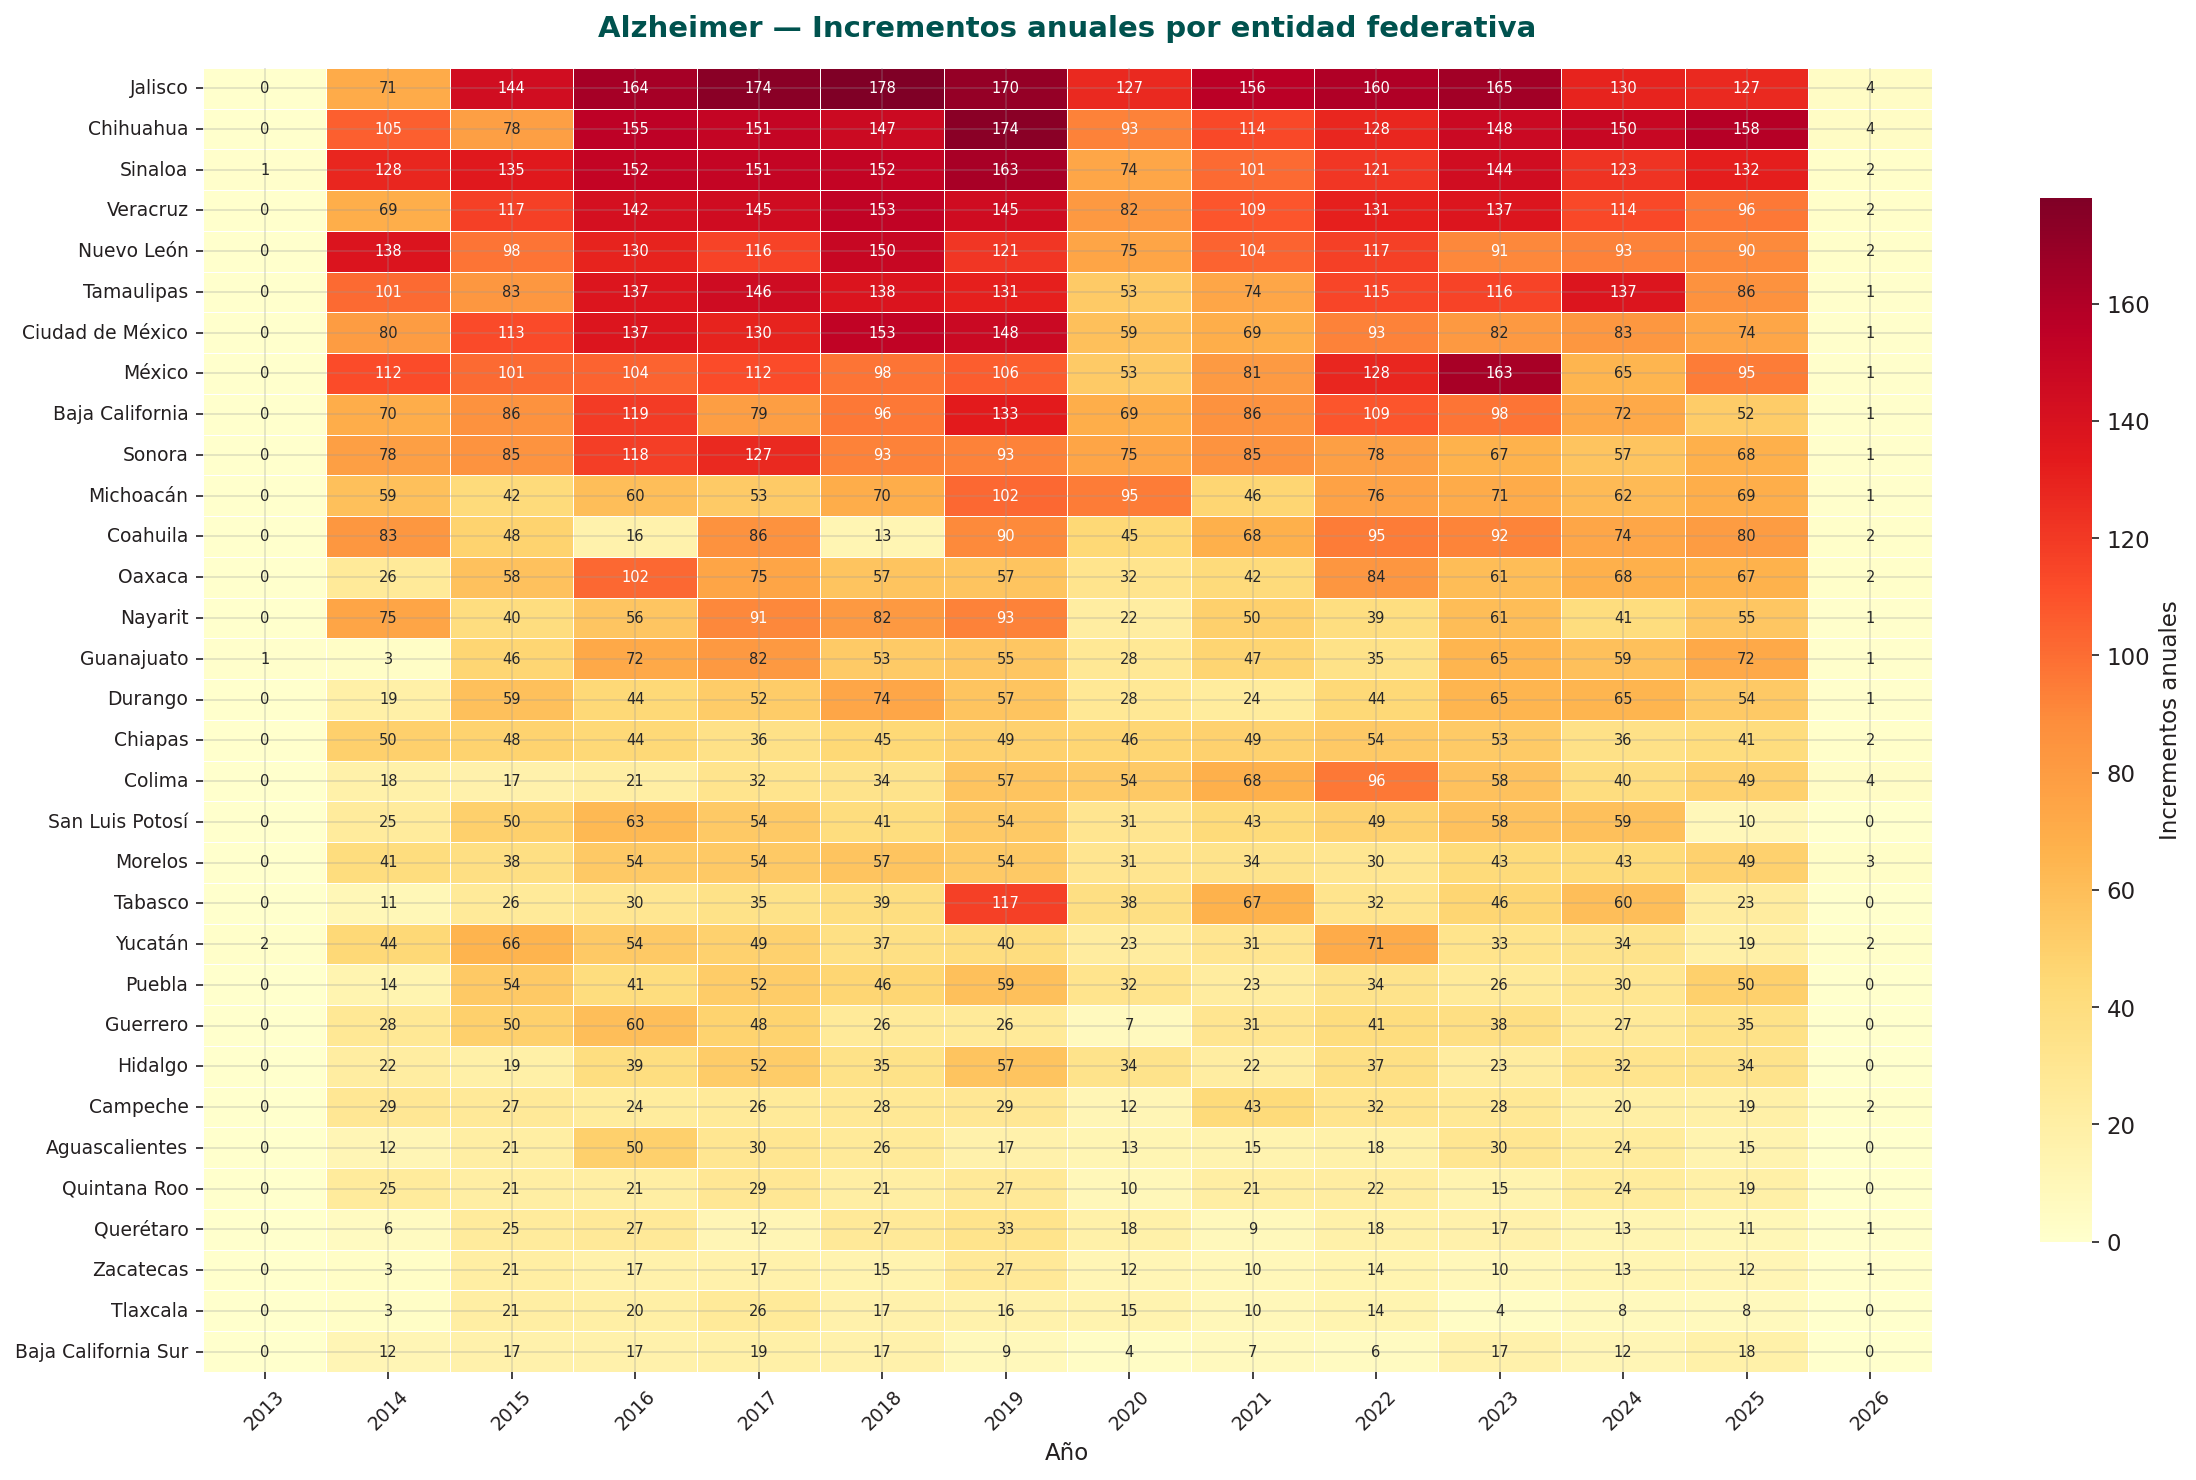
\includegraphics[width=\textwidth]{img/heatmap_entidad_anio_alzheimer.png}
    \caption{Alzheimer (G30) --- Incrementos anuales por entidad federativa.}
\end{figure}

% -------------------------------------------------------
\subsubsection{Series de tiempo de las entidades con mayor incidencia}

Para las 5 entidades con mayor carga total de cada padecimiento, se presenta la evolución temporal de incrementos semanales suavizados con media móvil de 8 semanas, permitiendo identificar estacionalidad, impacto COVID y tendencias individuales.

\begin{figure}[H]
    \centering
    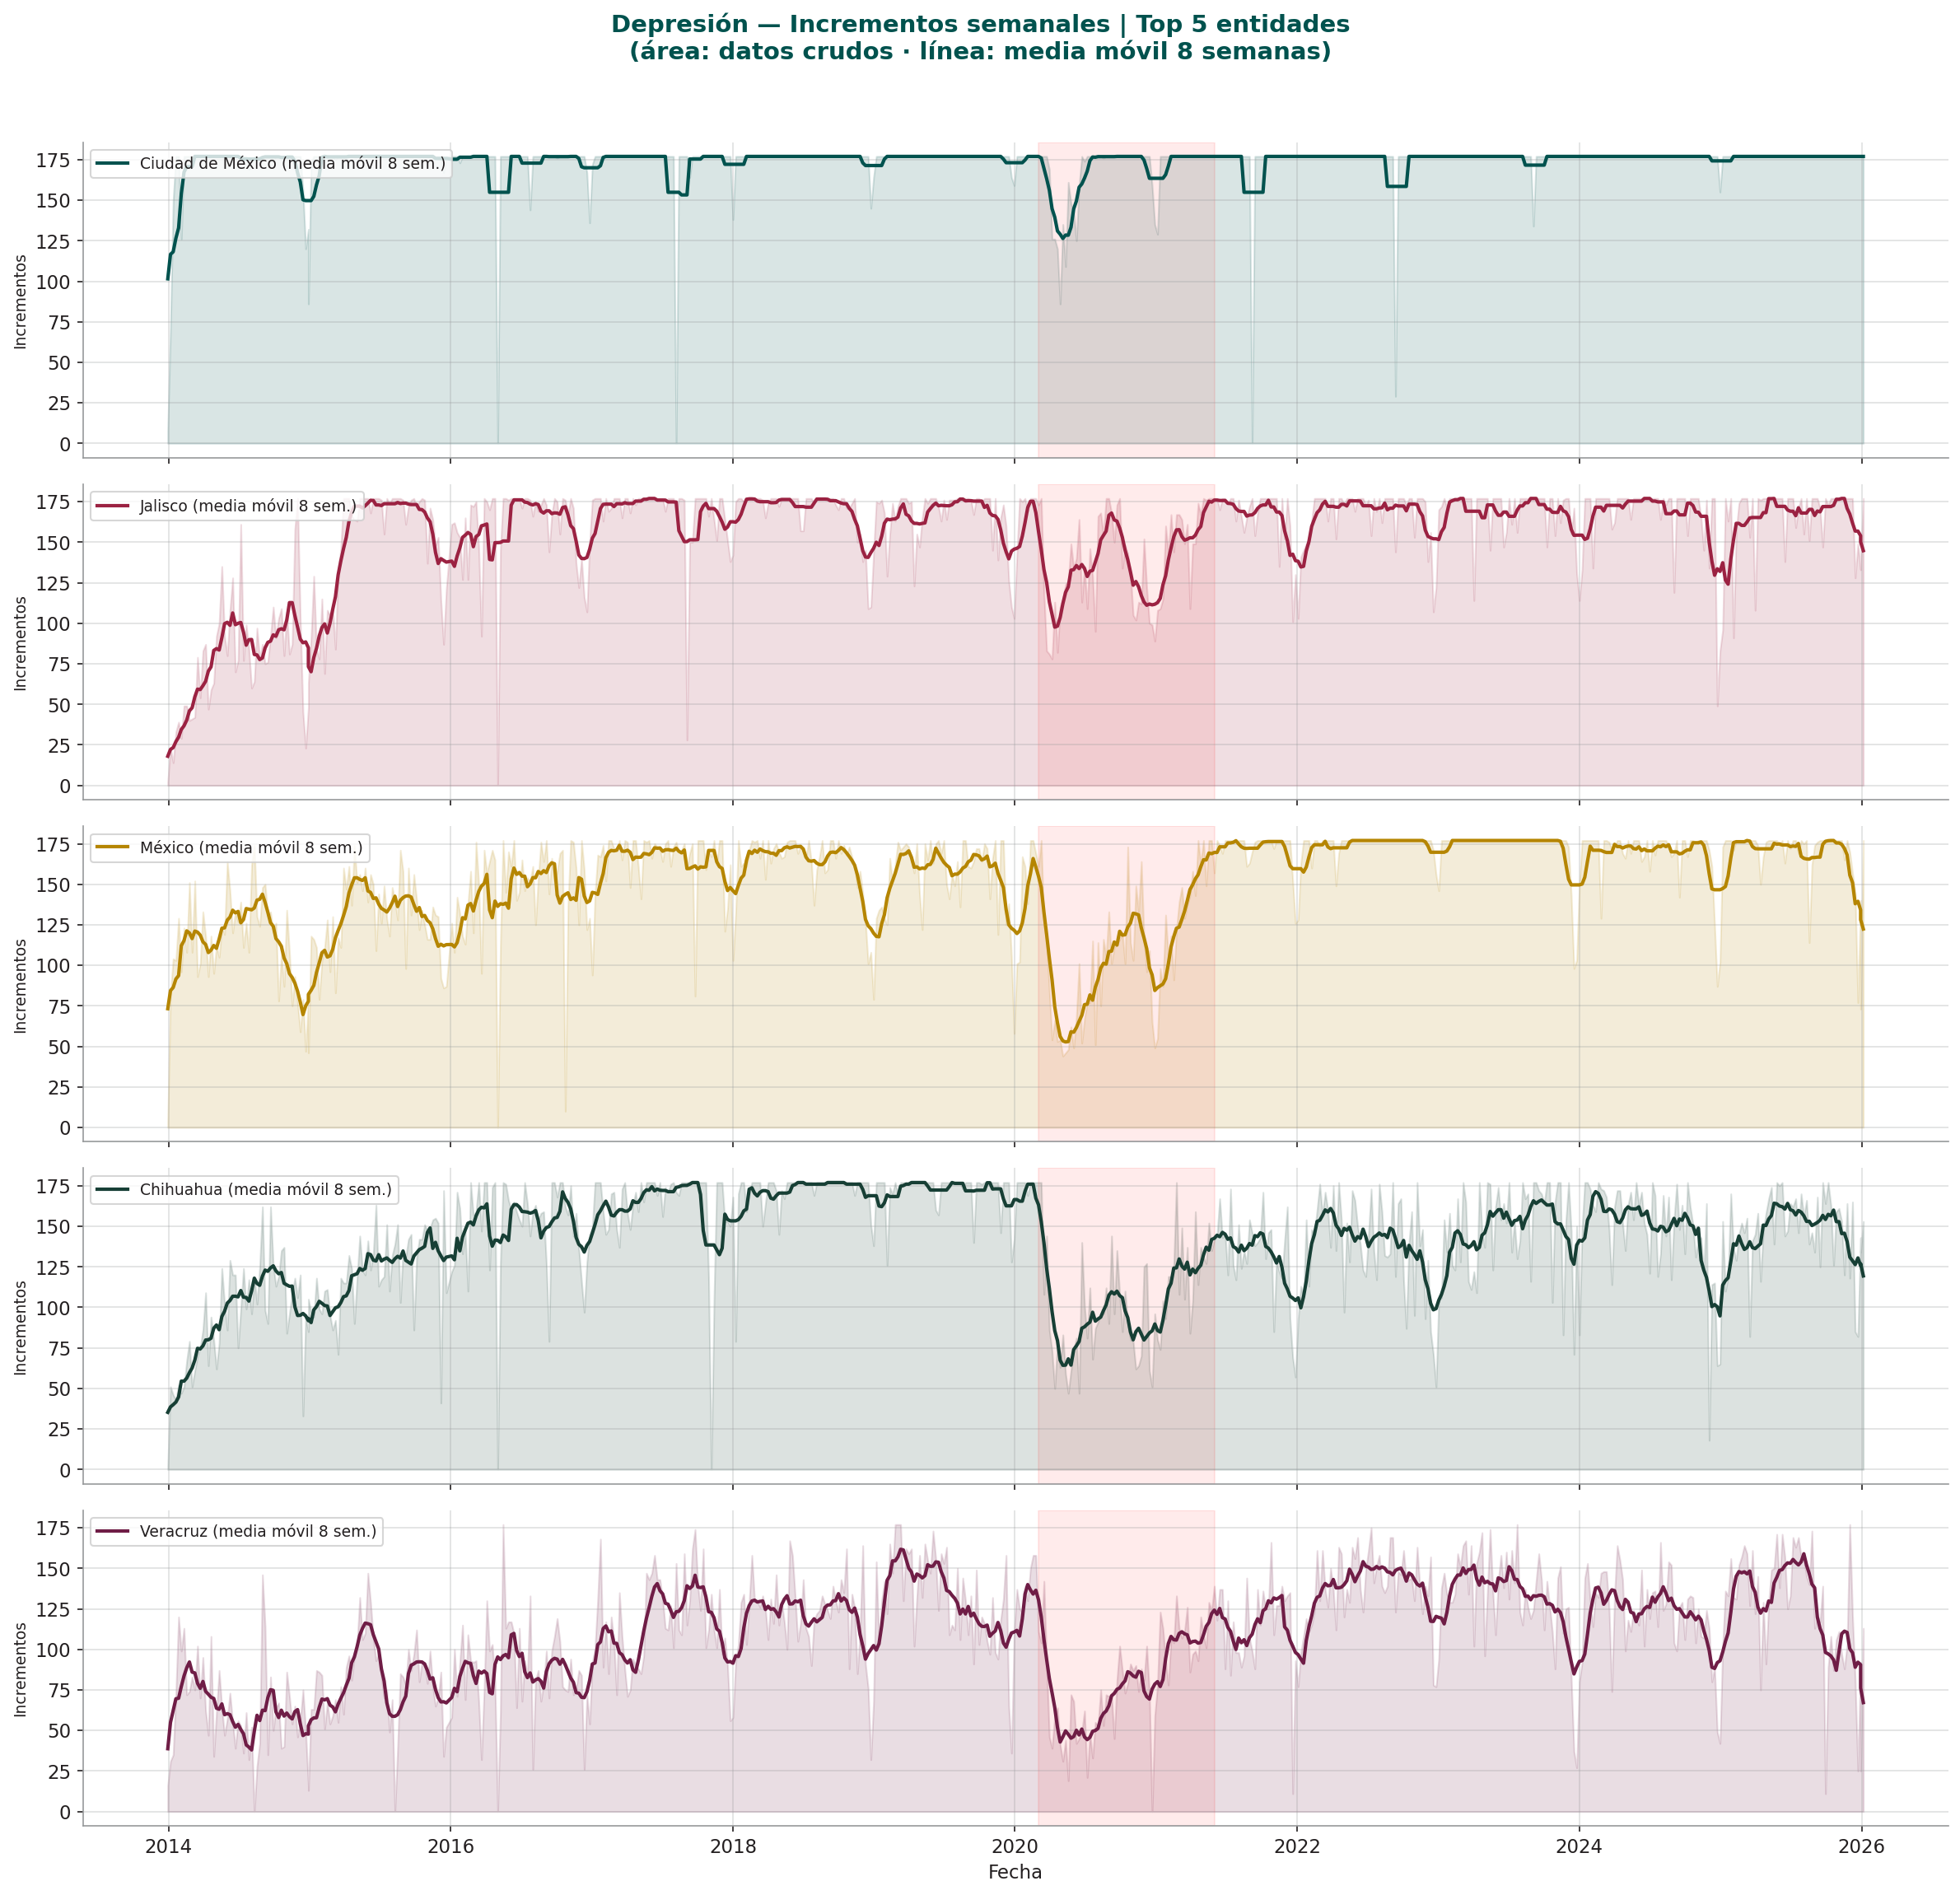
\includegraphics[width=\textwidth]{img/serie_top5_depresion.png}
    \caption{Depresión (F32) --- Incrementos semanales, top 5 entidades.}
\end{figure}

\begin{figure}[H]
    \centering
    
\includegraphics[width=\textwidth]{img/serie_top5_parkinson.png}
    \caption{Parkinson (G20) --- Incrementos semanales, top 5 entidades.}
\end{figure}

\begin{figure}[H]
    \centering
    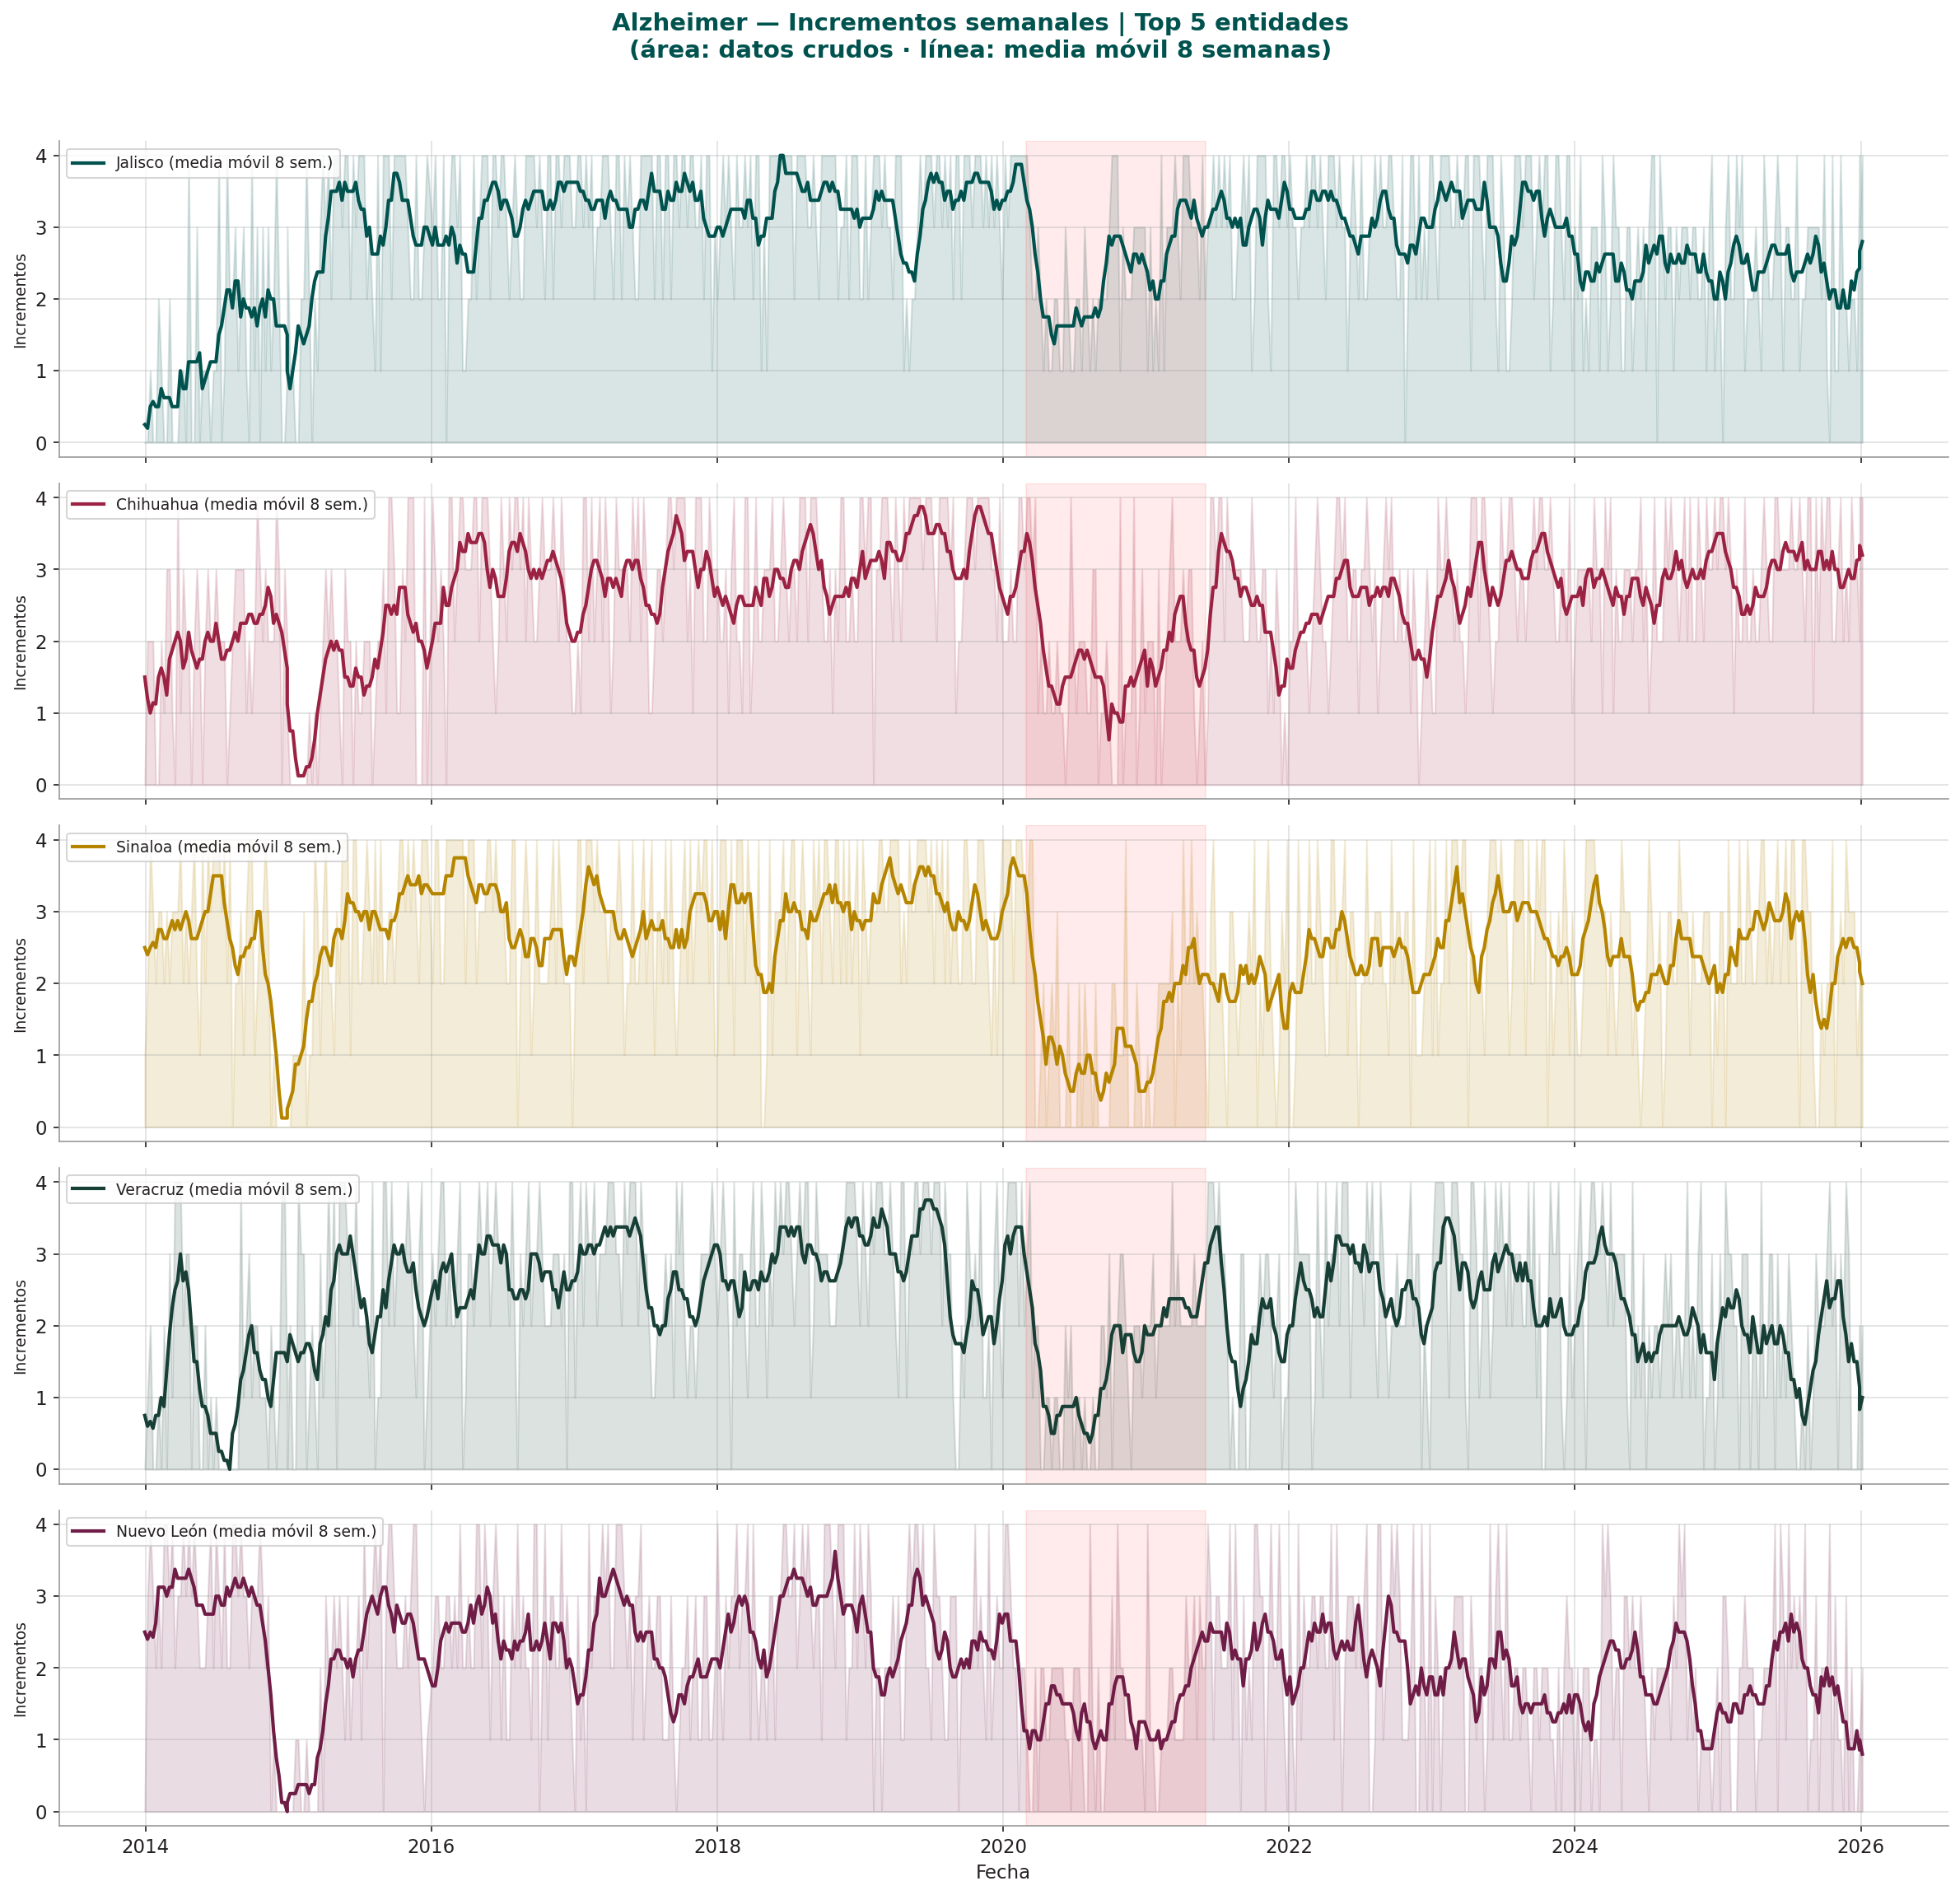
\includegraphics[width=\textwidth]{img/serie_top5_alzheimer.png}
    \caption{Alzheimer (G30) --- Incrementos semanales, top 5 entidades.}
\end{figure}

% -------------------------------------------------------
\subsubsection{Panorama completo: Series de tiempo por entidad federativa}

A diferencia de las secciones anteriores, aquí se presenta la \textbf{evolución temporal individual de las 32 entidades federativas} para cada padecimiento. Las series están ordenadas de mayor a menor carga acumulada y suavizadas mediante una media móvil de 8 semanas para facilitar la lectura de tendencias. Este desglose permite identificar qué estados concentran los volúmenes más altos, cuáles muestran estacionalidad marcada, dónde el impacto COVID fue más severo y qué entidades presentan trayectorias atípicas.

\begin{figure}[H]
    \centering
    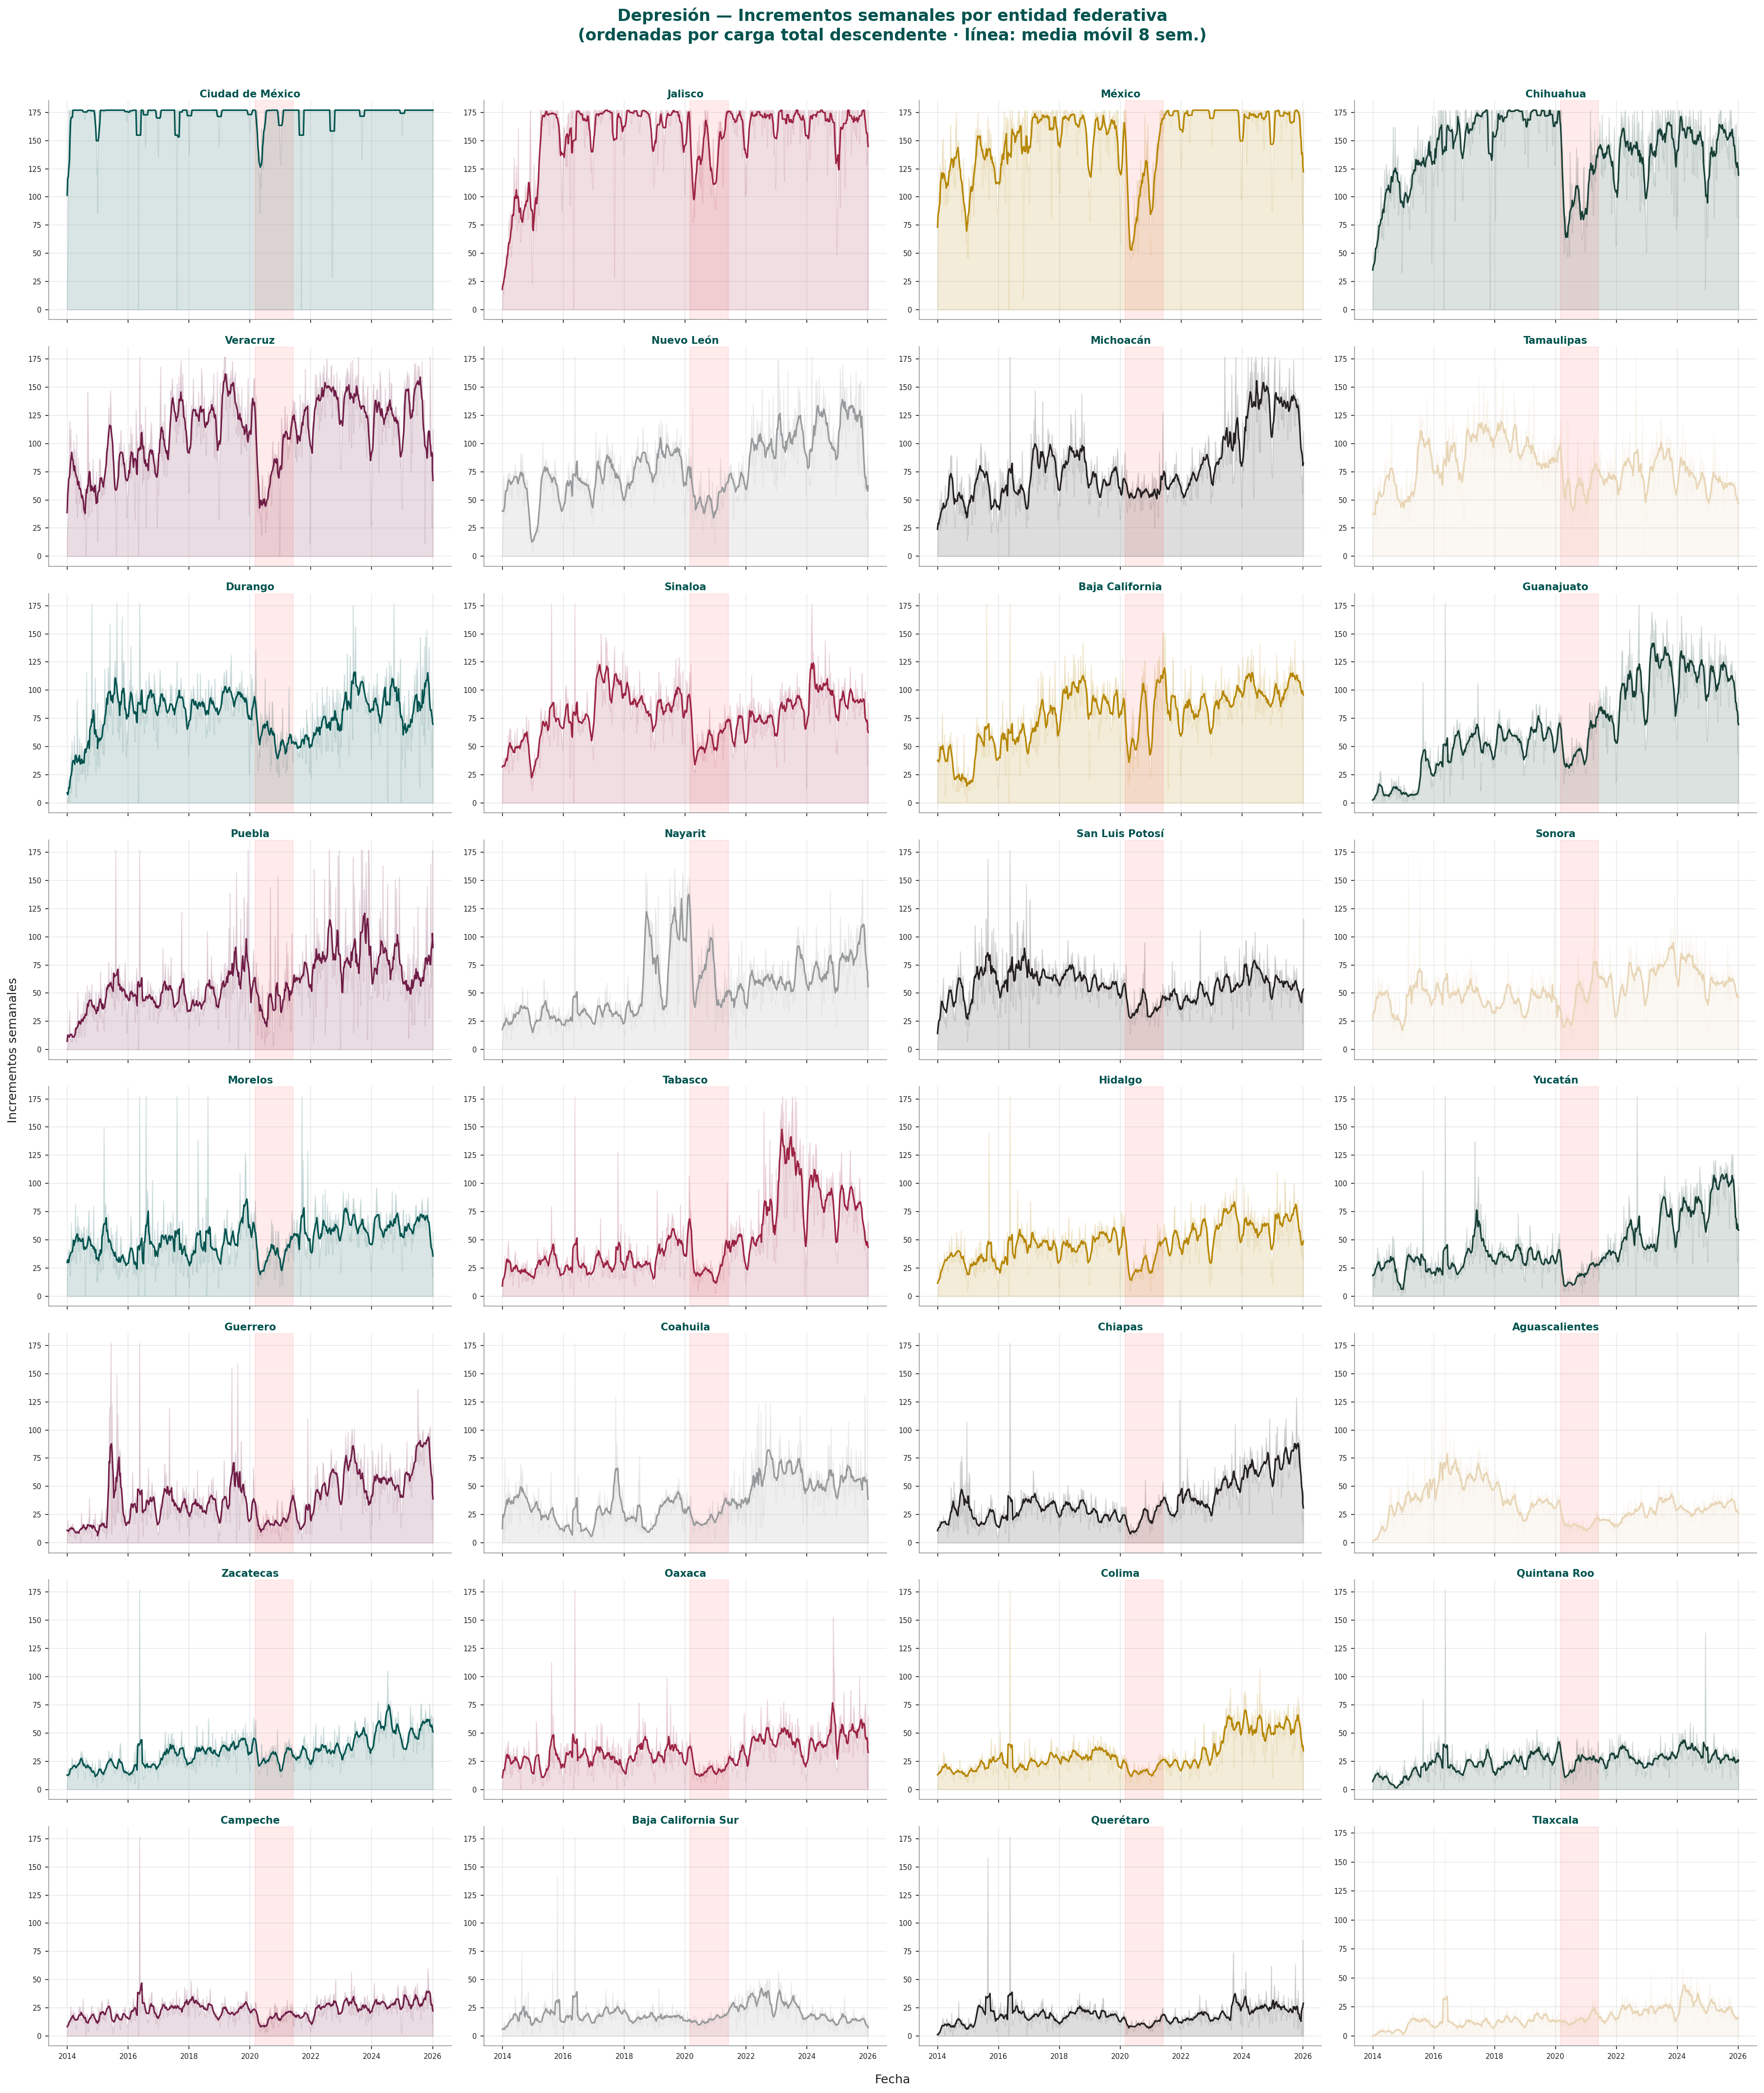
\includegraphics[width=\textwidth]{img/serie_todas_entidades_depresion.png}
    \caption{Depresión (F32) --- Incrementos semanales, 32 entidades federativas.}
\end{figure}

\begin{figure}[H]
    \centering
    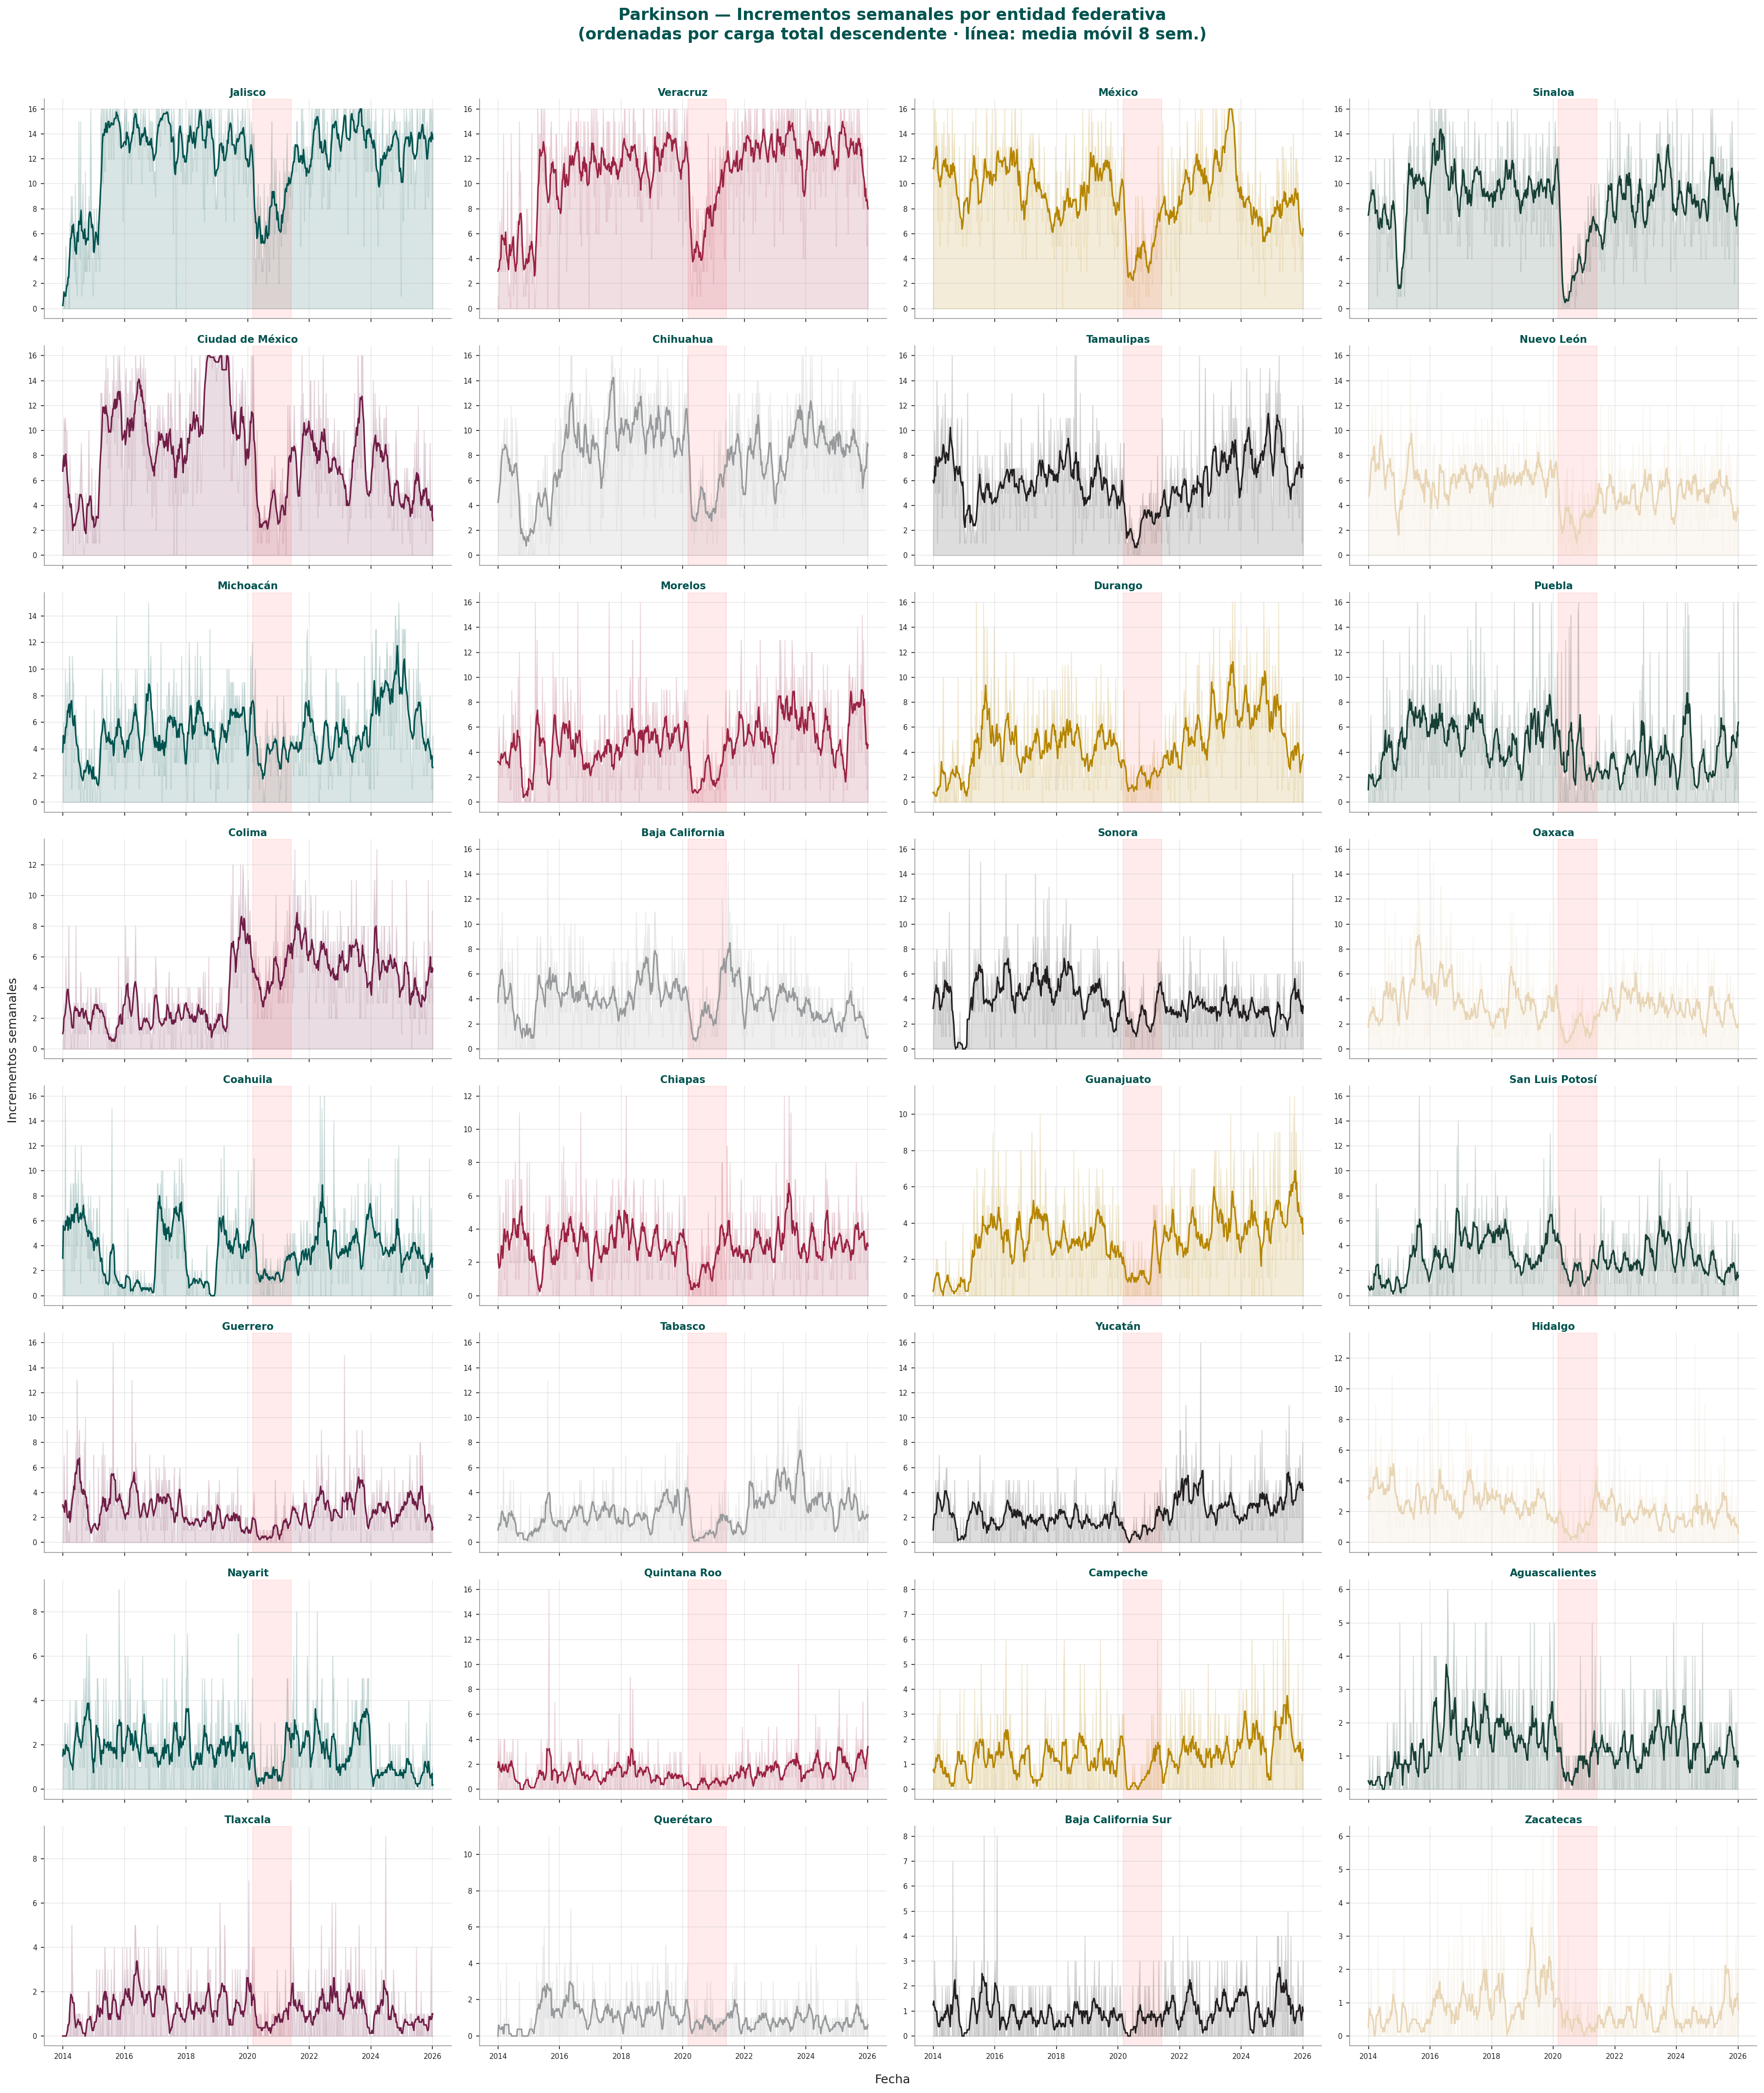
\includegraphics[width=\textwidth]{img/serie_todas_entidades_parkinson.png}
    \caption{Parkinson (G20) --- Incrementos semanales, 32 entidades federativas.}
\end{figure}

\begin{figure}[H]
    \centering
    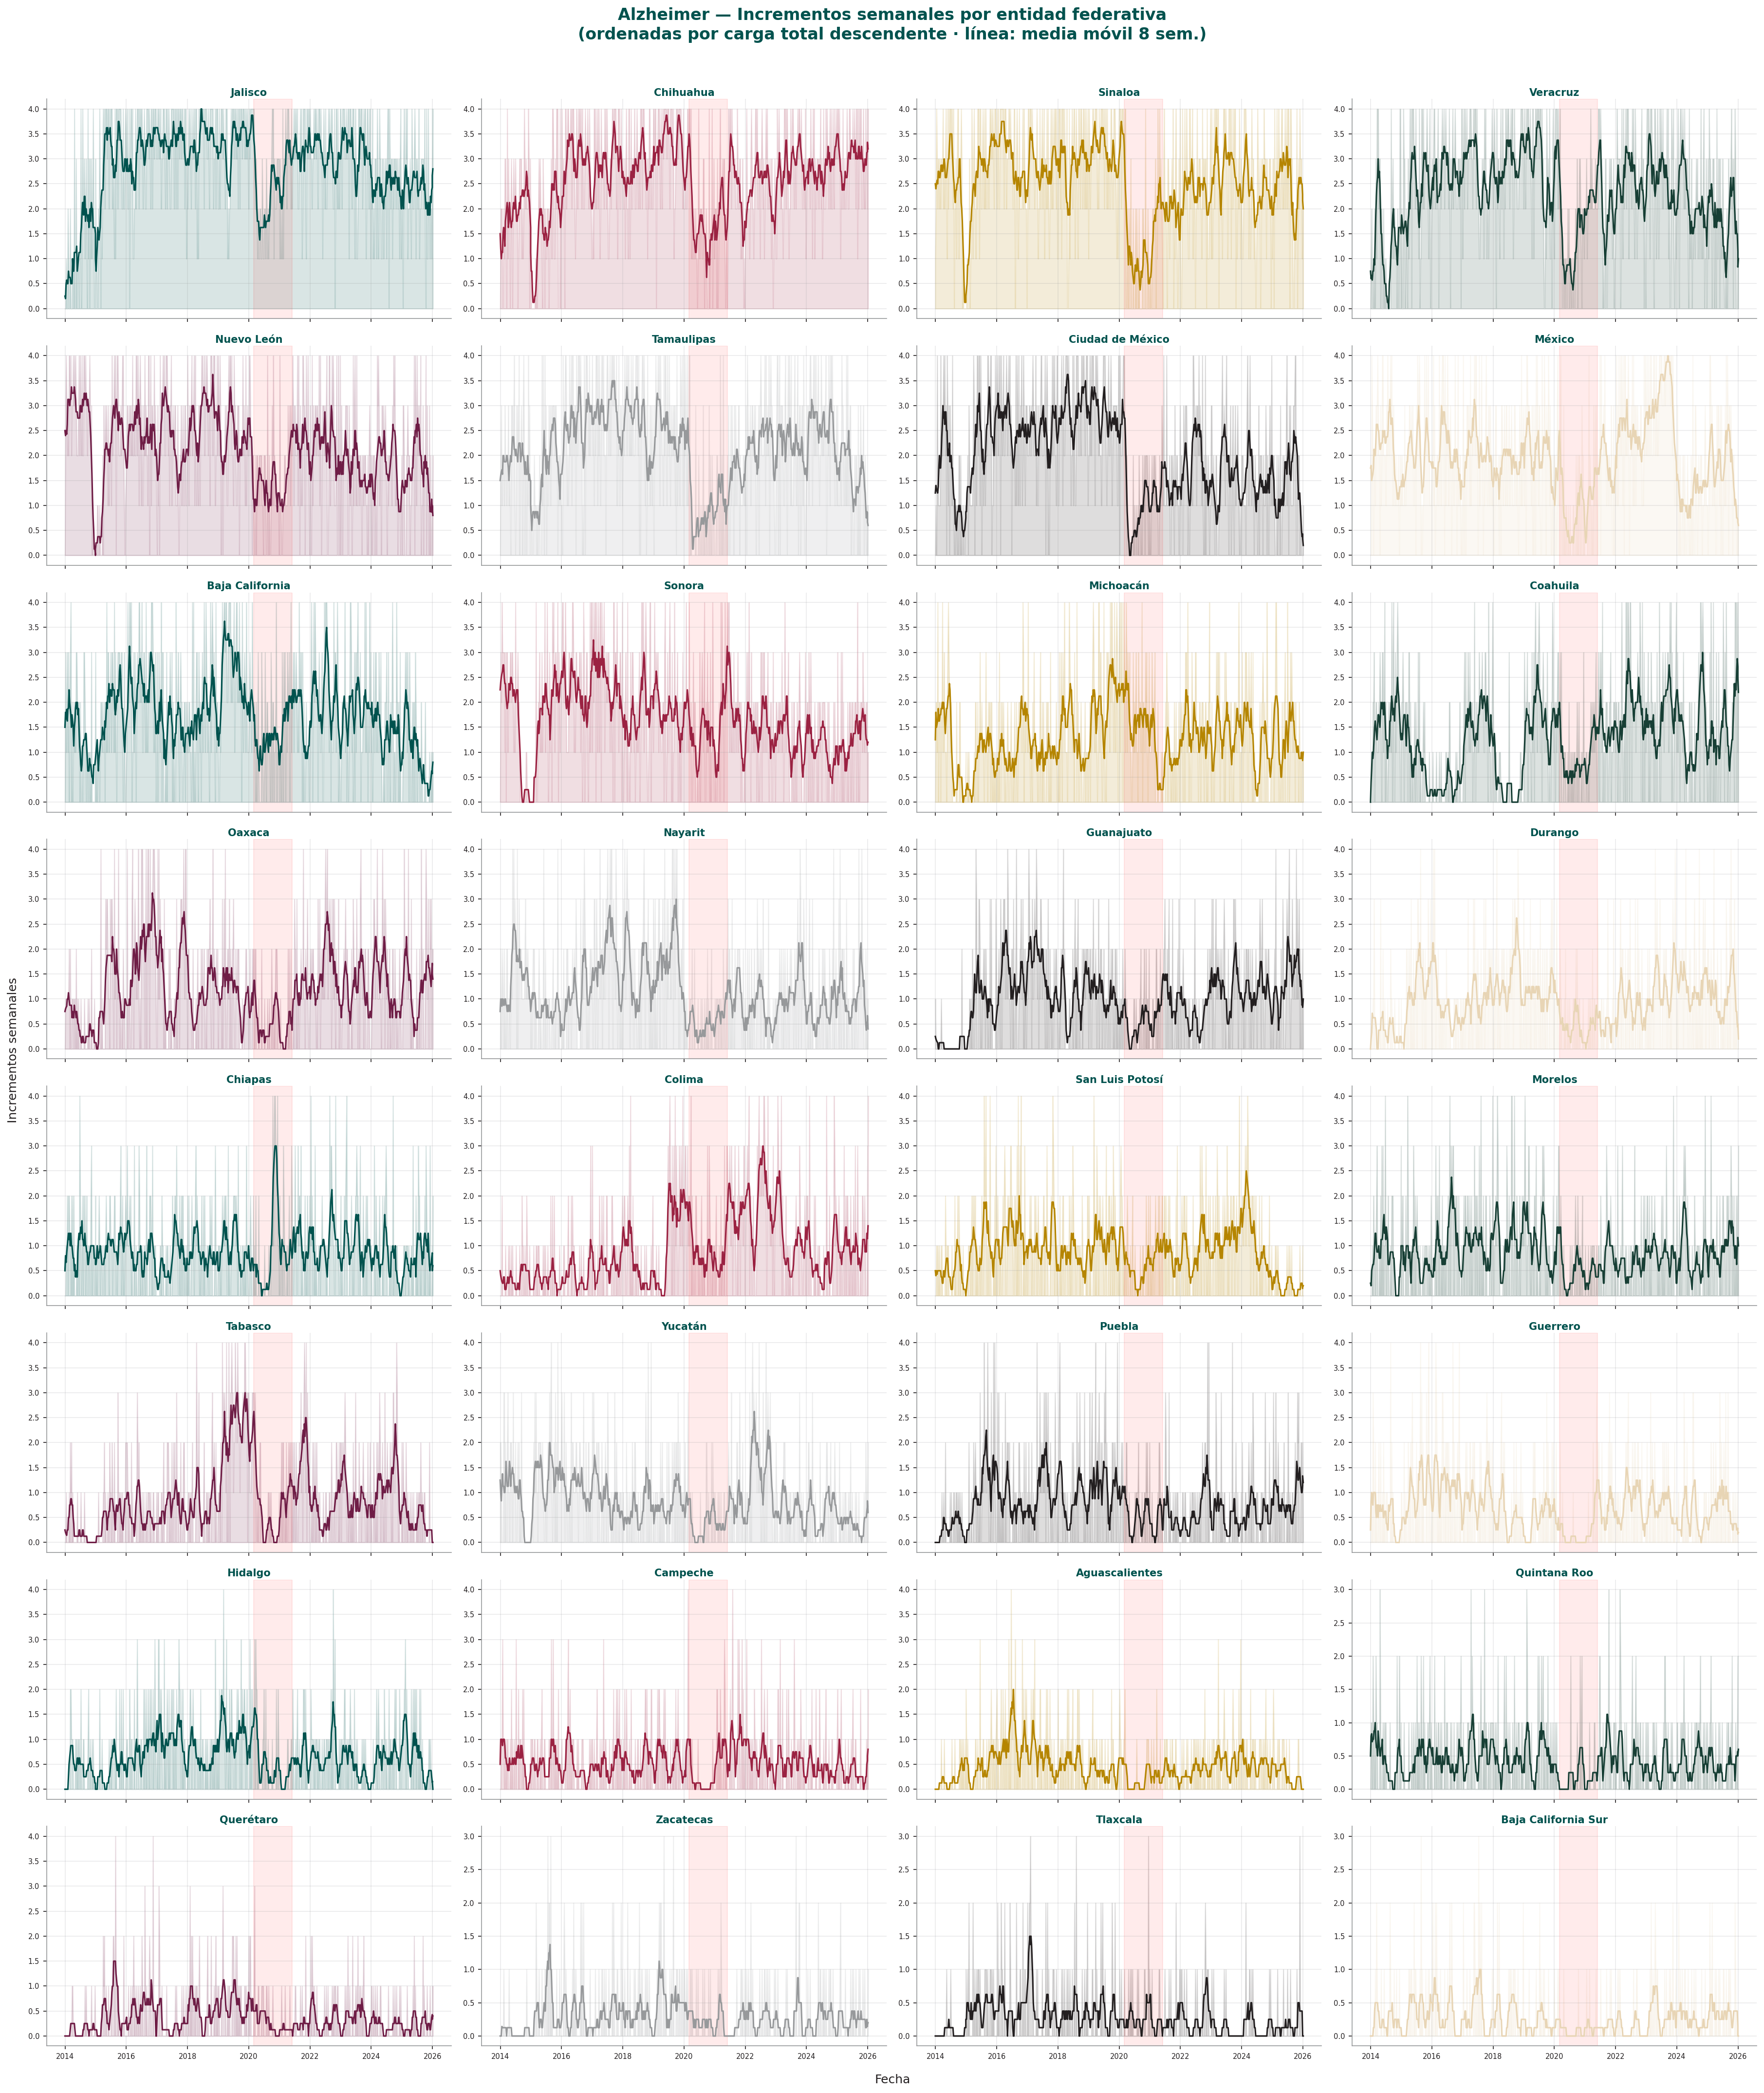
\includegraphics[width=\textwidth]{img/serie_todas_entidades_alzheimer.png}
    \caption{Alzheimer (G30) --- Incrementos semanales, 32 entidades federativas.}
\end{figure}

% -------------------------------------------------------
\subsubsection{Desagregación por sexo a nivel entidad federativa}

Complementando el panorama general, se presenta la misma visualización de las 32 entidades con la \textbf{desagregación por sexo} superpuesta en cada panel. La línea teal representa hombres y la burgundy mujeres, permitiendo identificar la magnitud de la brecha de género en el reporte epidemiológico, si el patrón temporal difiere entre sexos y qué entidades presentan proporciones atípicas respecto al promedio nacional.

\begin{figure}[H]
    \centering
    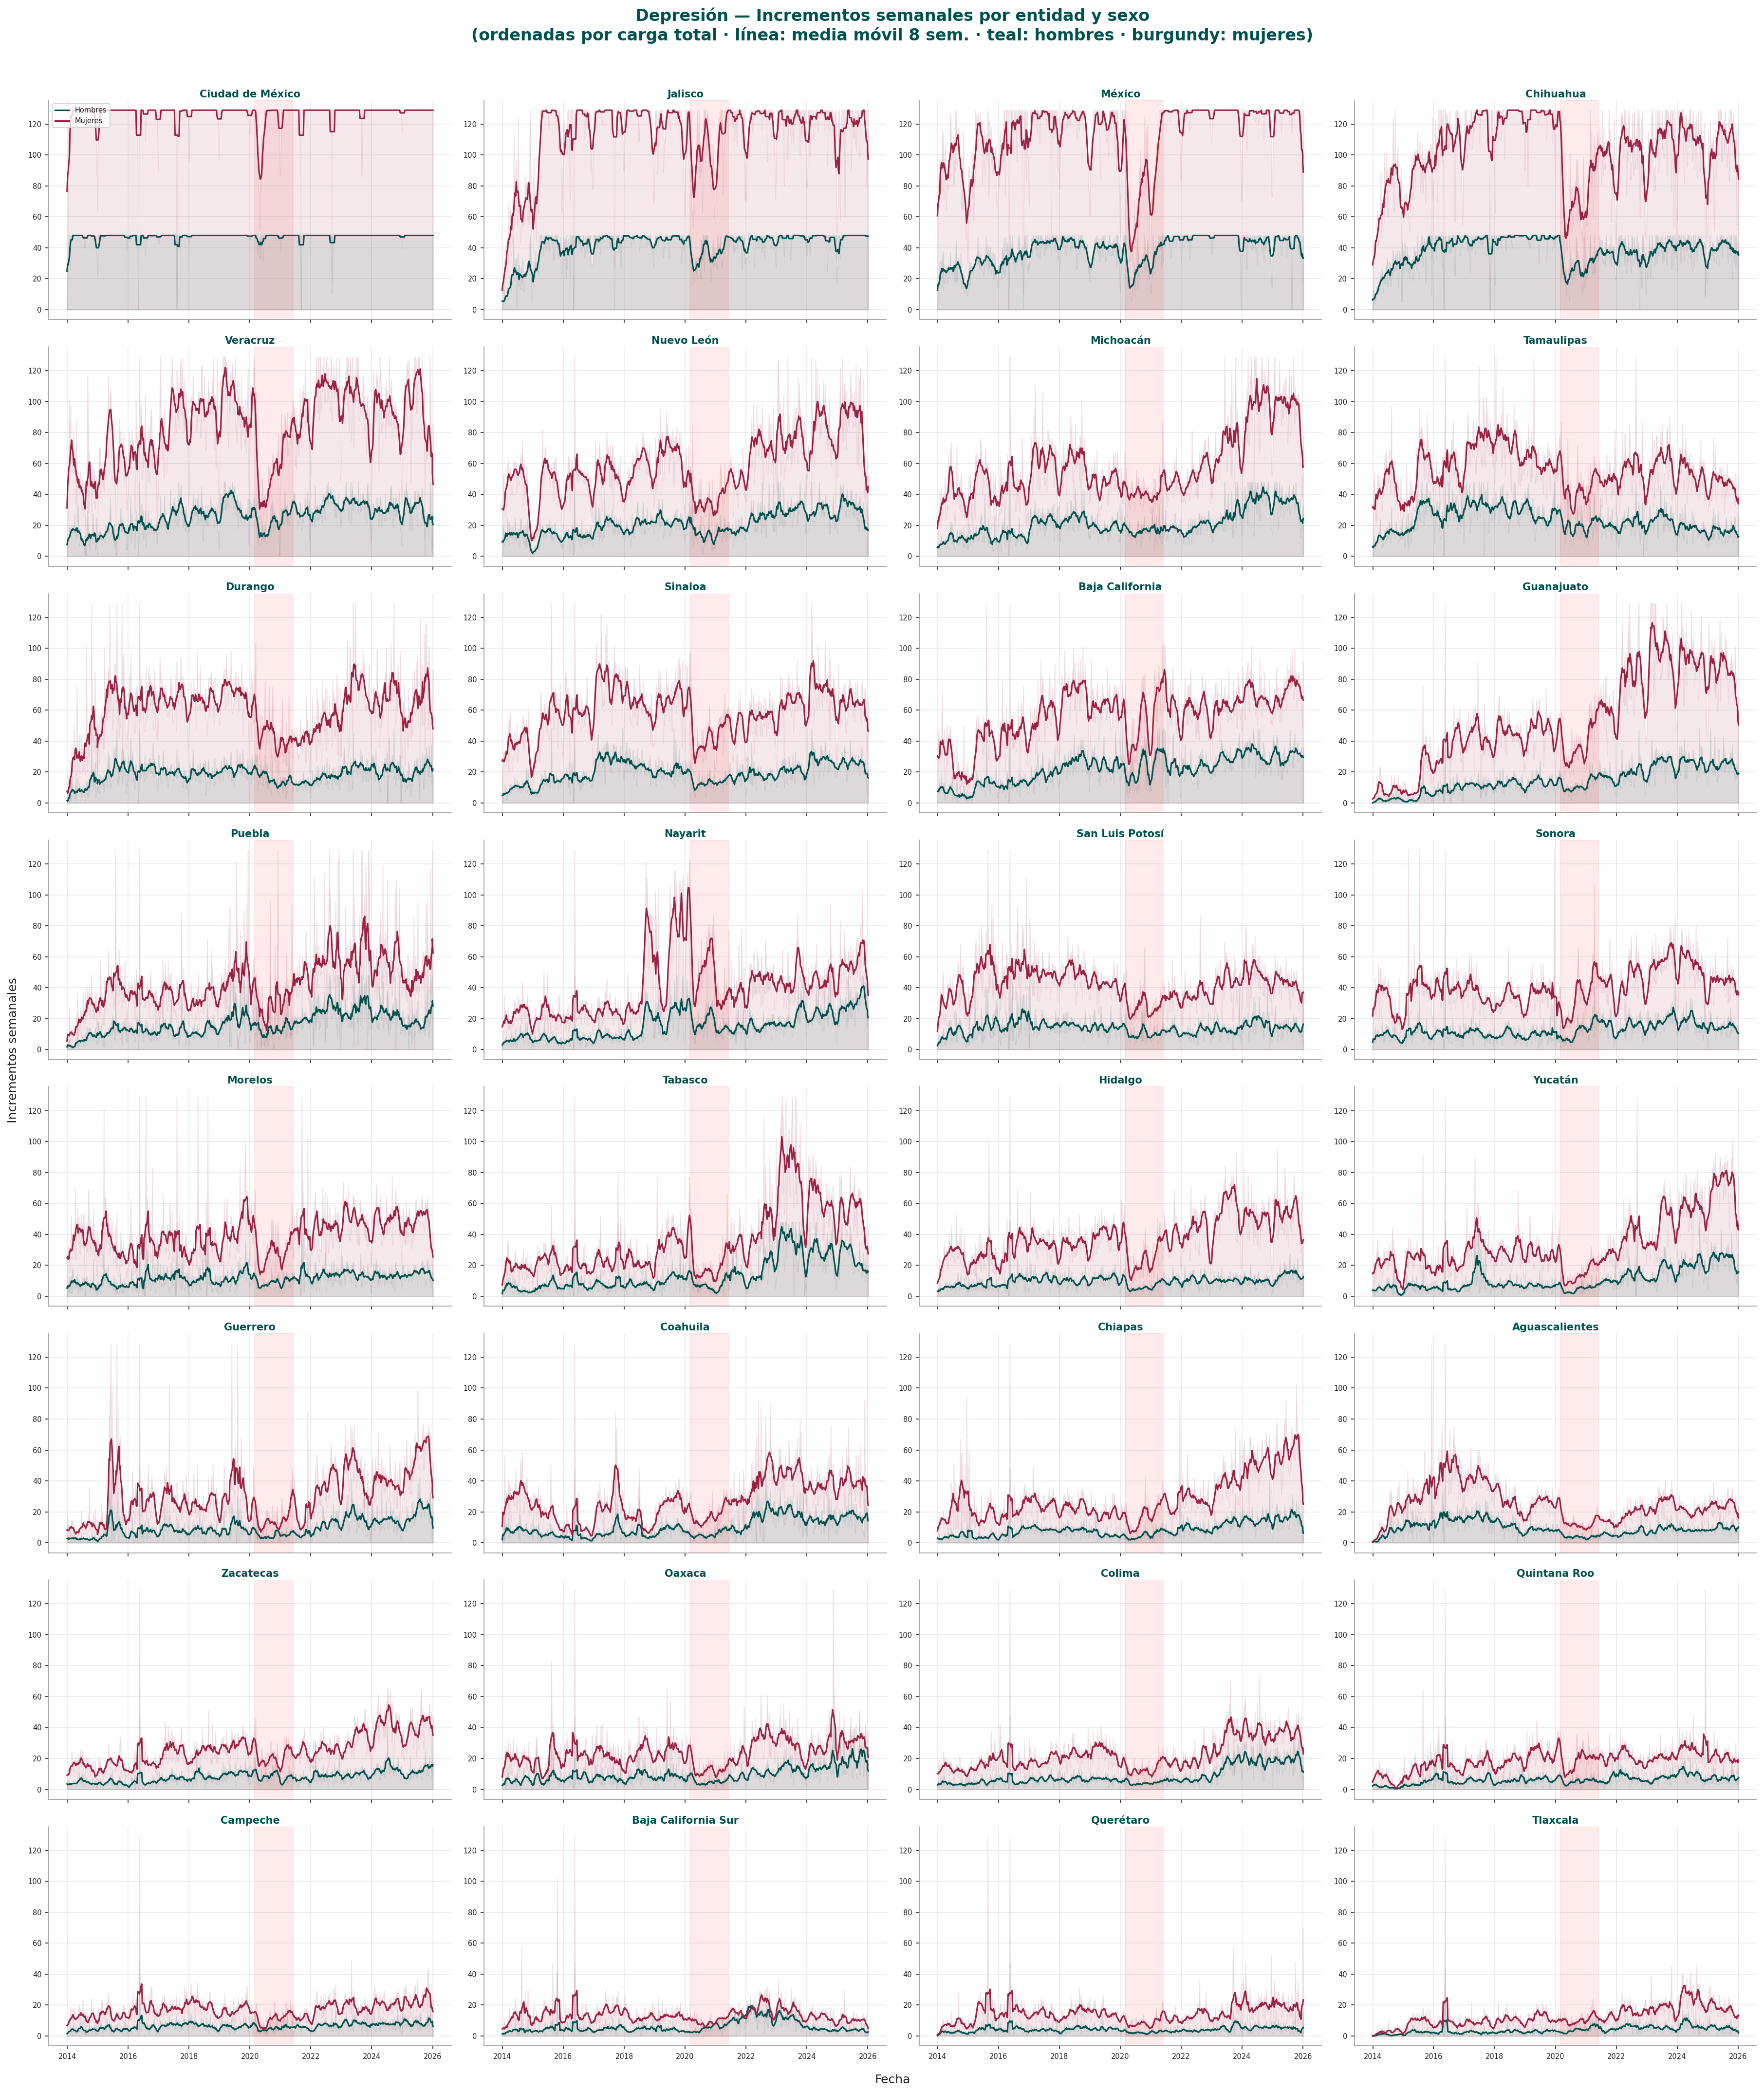
\includegraphics[width=\textwidth]{img/serie_todas_entidades_sexo_depresion.png}
    \caption{Depresión (F32) --- Incrementos semanales por sexo, 32 entidades.}
\end{figure}

\begin{figure}[H]
    \centering
    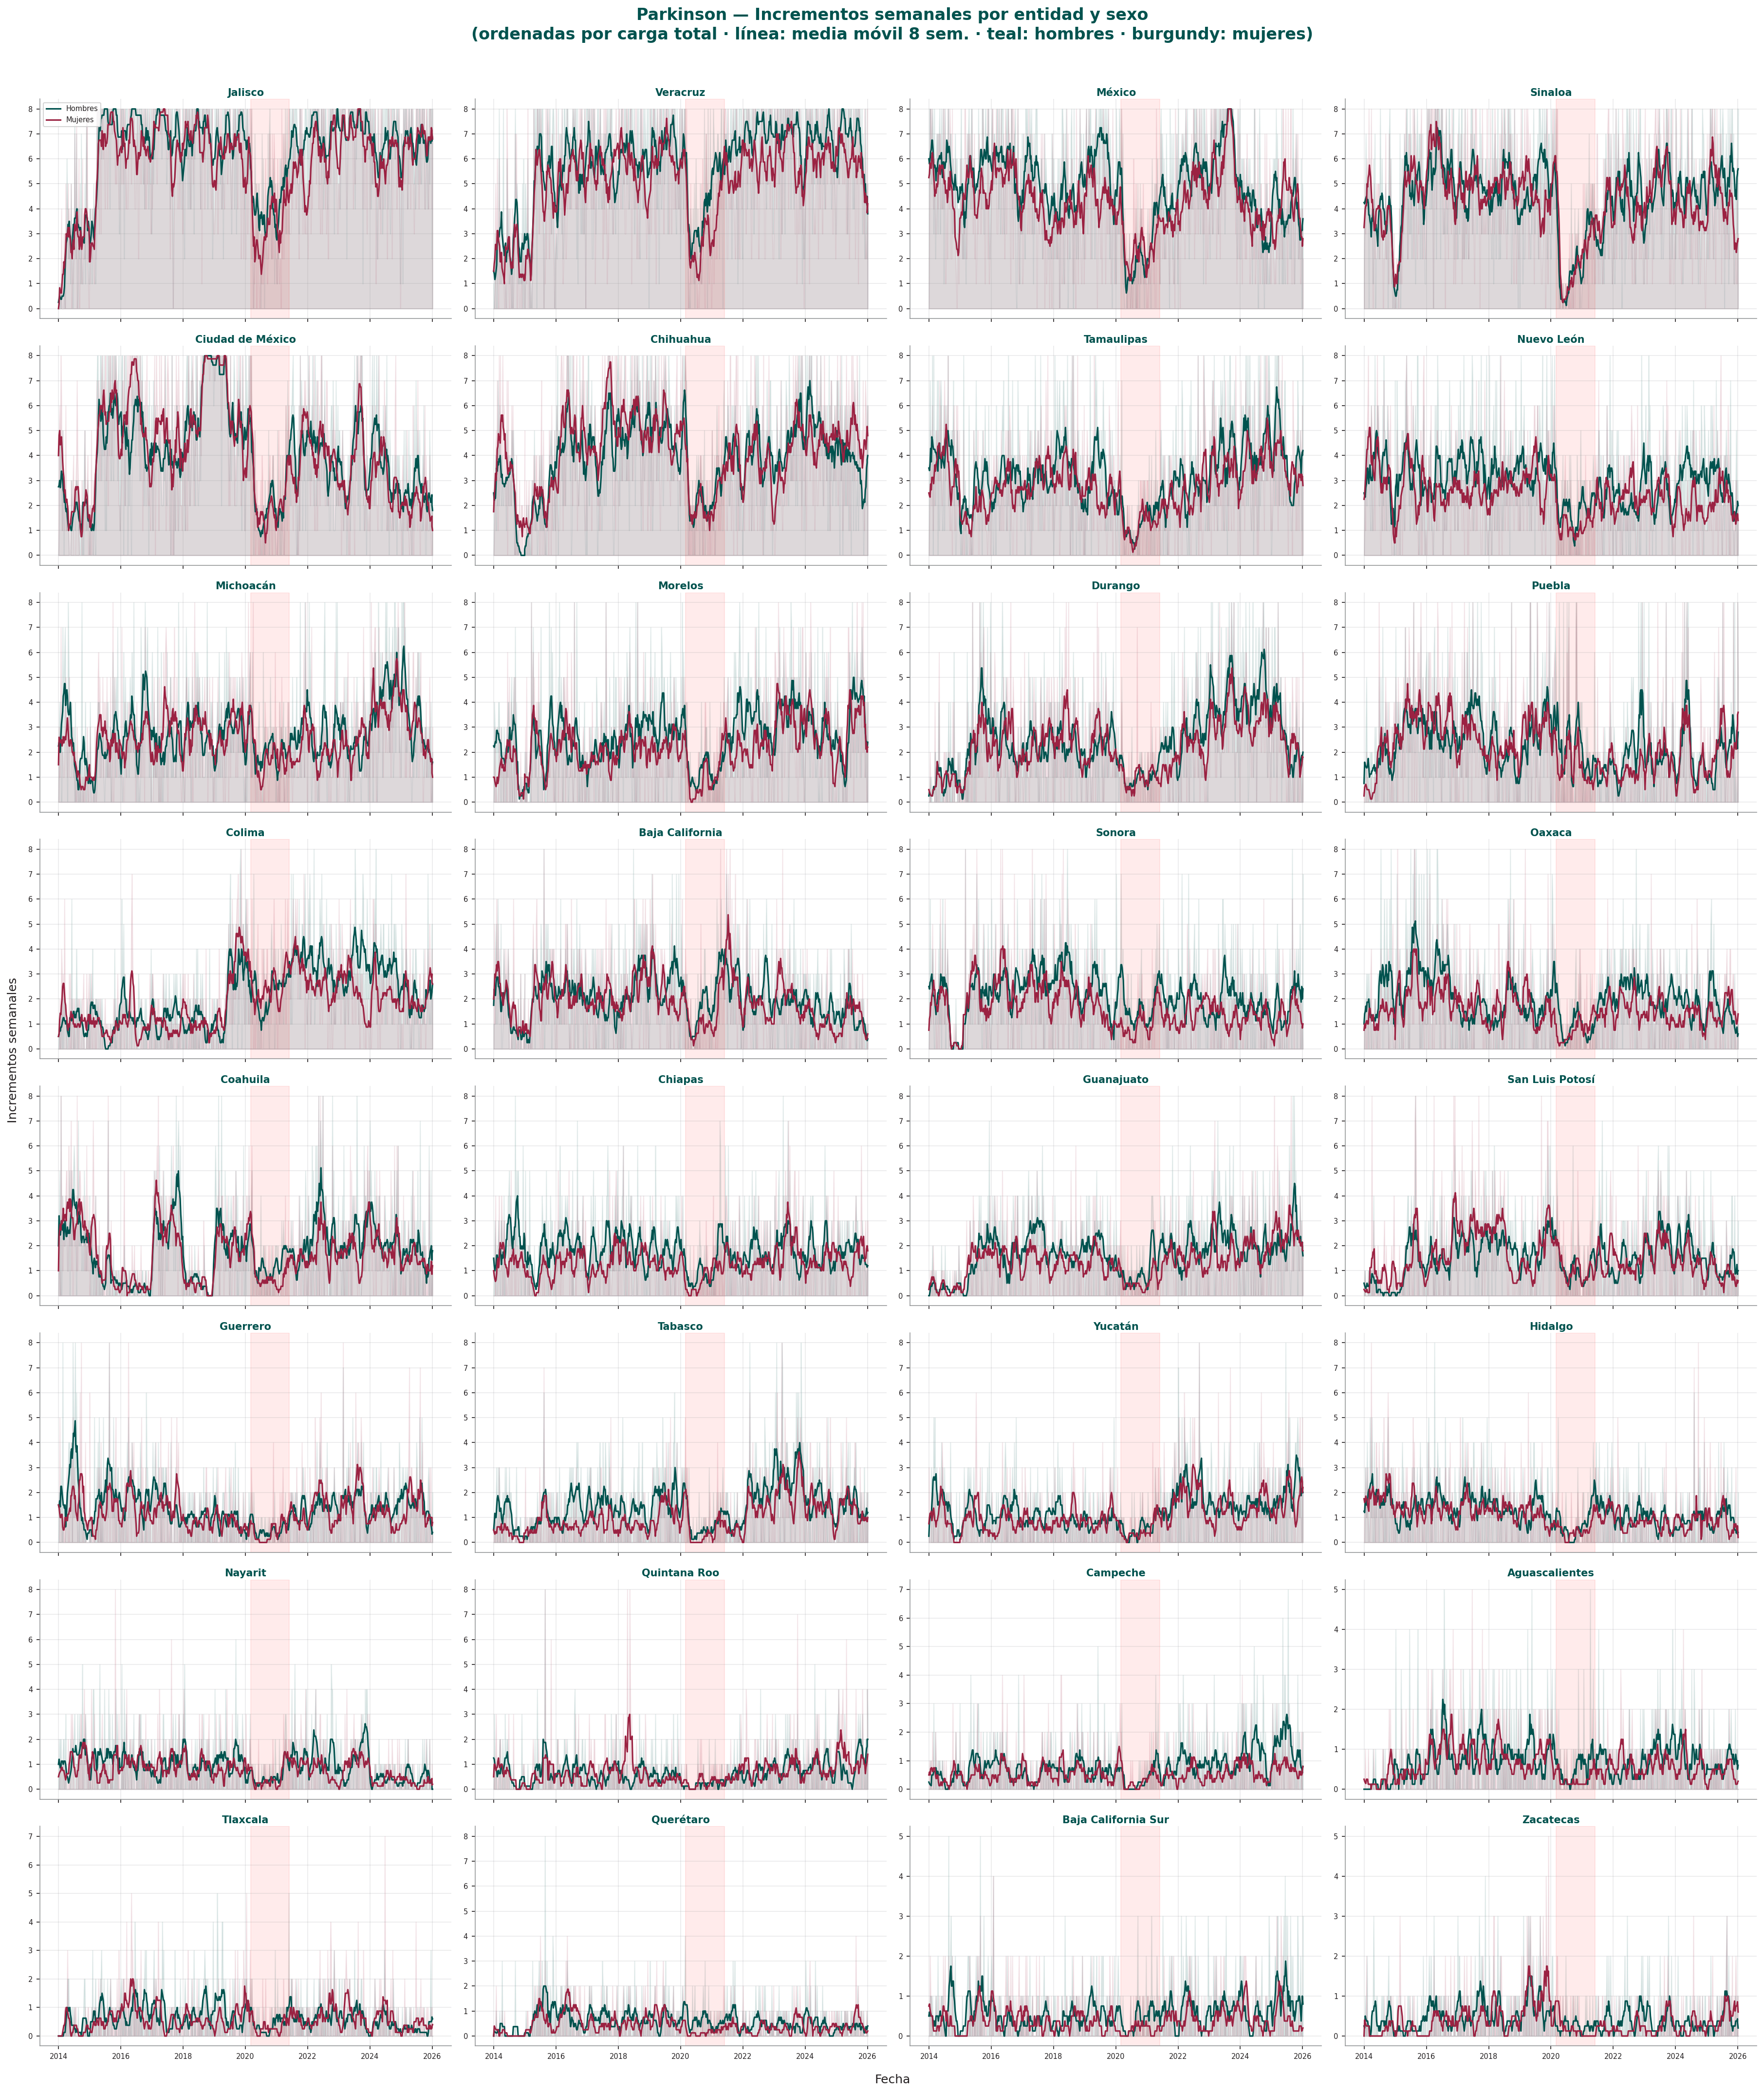
\includegraphics[width=\textwidth]{img/serie_todas_entidades_sexo_parkinson.png}
    \caption{Parkinson (G20) --- Incrementos semanales por sexo, 32 entidades.}
\end{figure}

\begin{figure}[H]
    \centering
    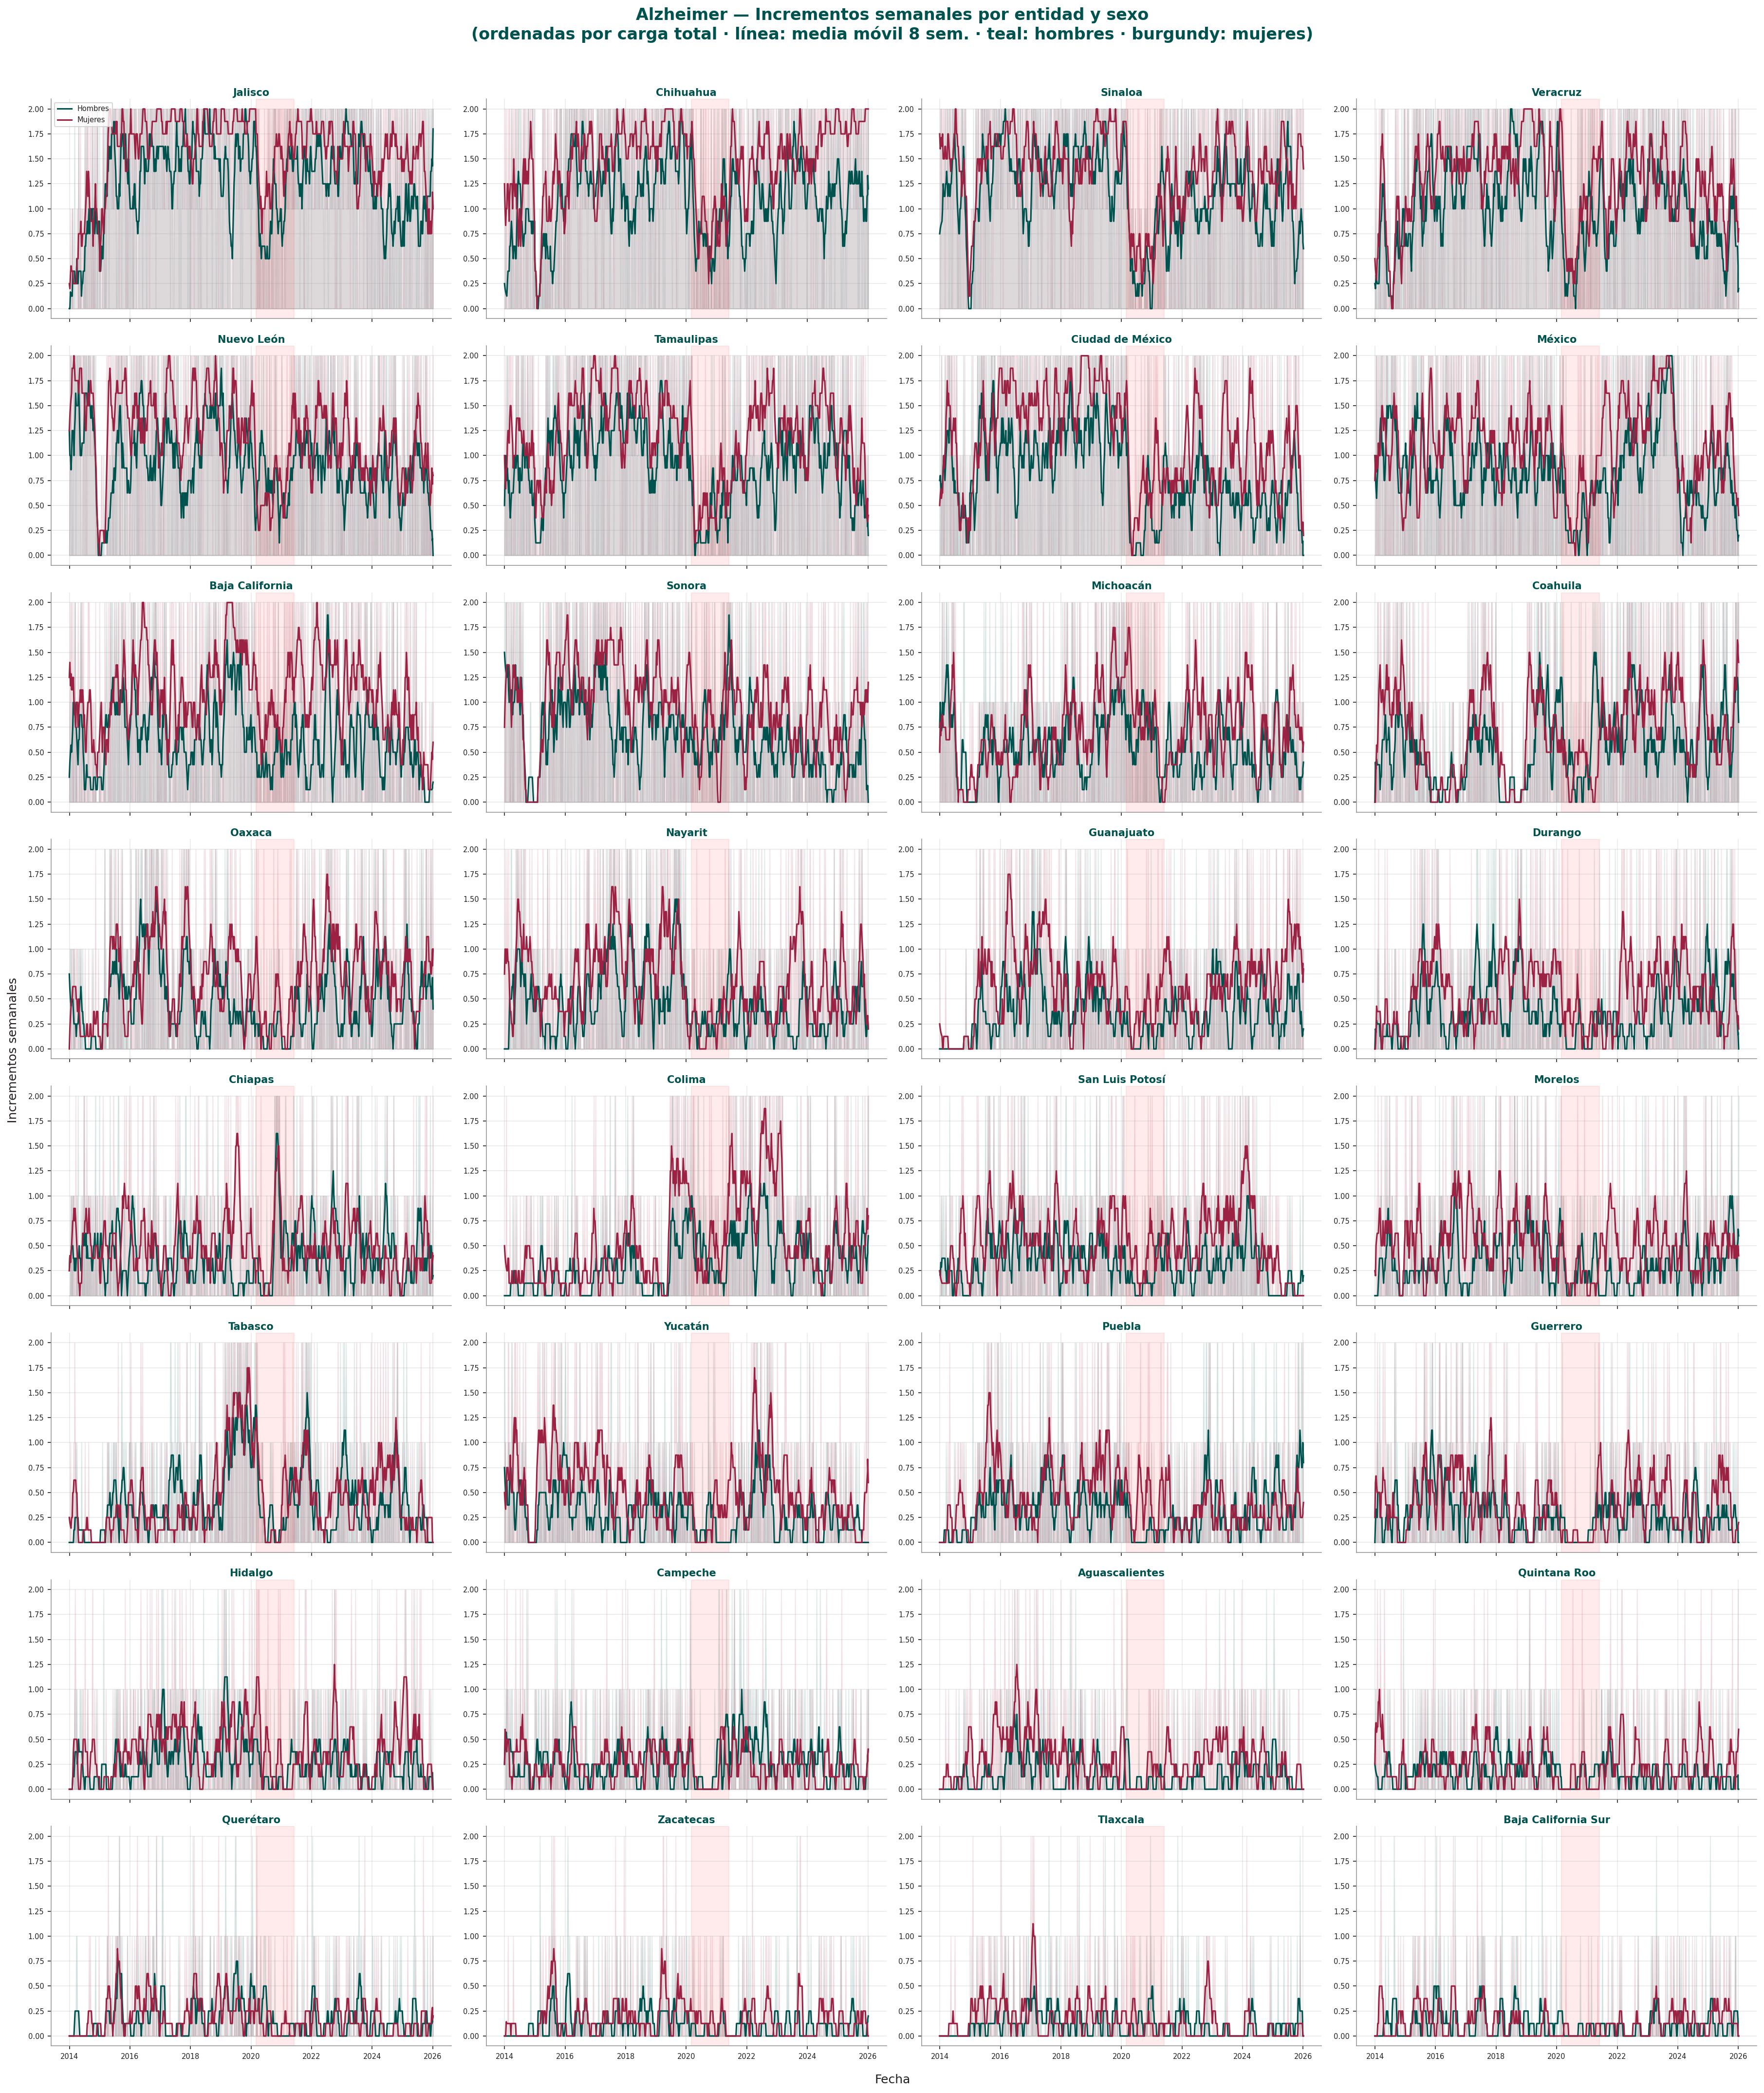
\includegraphics[width=\textwidth]{img/serie_todas_entidades_sexo_alzheimer.png}
    \caption{Alzheimer (G30) --- Incrementos semanales por sexo, 32 entidades.}
\end{figure}

% -------------------------------------------------------
\subsubsection{Evolución del ranking estatal a lo largo del tiempo}

¿Los mismos estados han dominado siempre el reporte de casos o hay movimientos significativos entre años? El \textbf{bump chart} responde esta pregunta: cada línea representa una de las 5 entidades con mayor carga histórica y su posición vertical indica su lugar en el ranking nacional. Los cruces de líneas revelan cambios de posición, y las trayectorias ascendentes o descendentes exponen tendencias de mediano plazo que podrían reflejar mejoras en cobertura diagnóstica, cambios demográficos o efectos de la pandemia.

\begin{figure}[H]
    \centering
    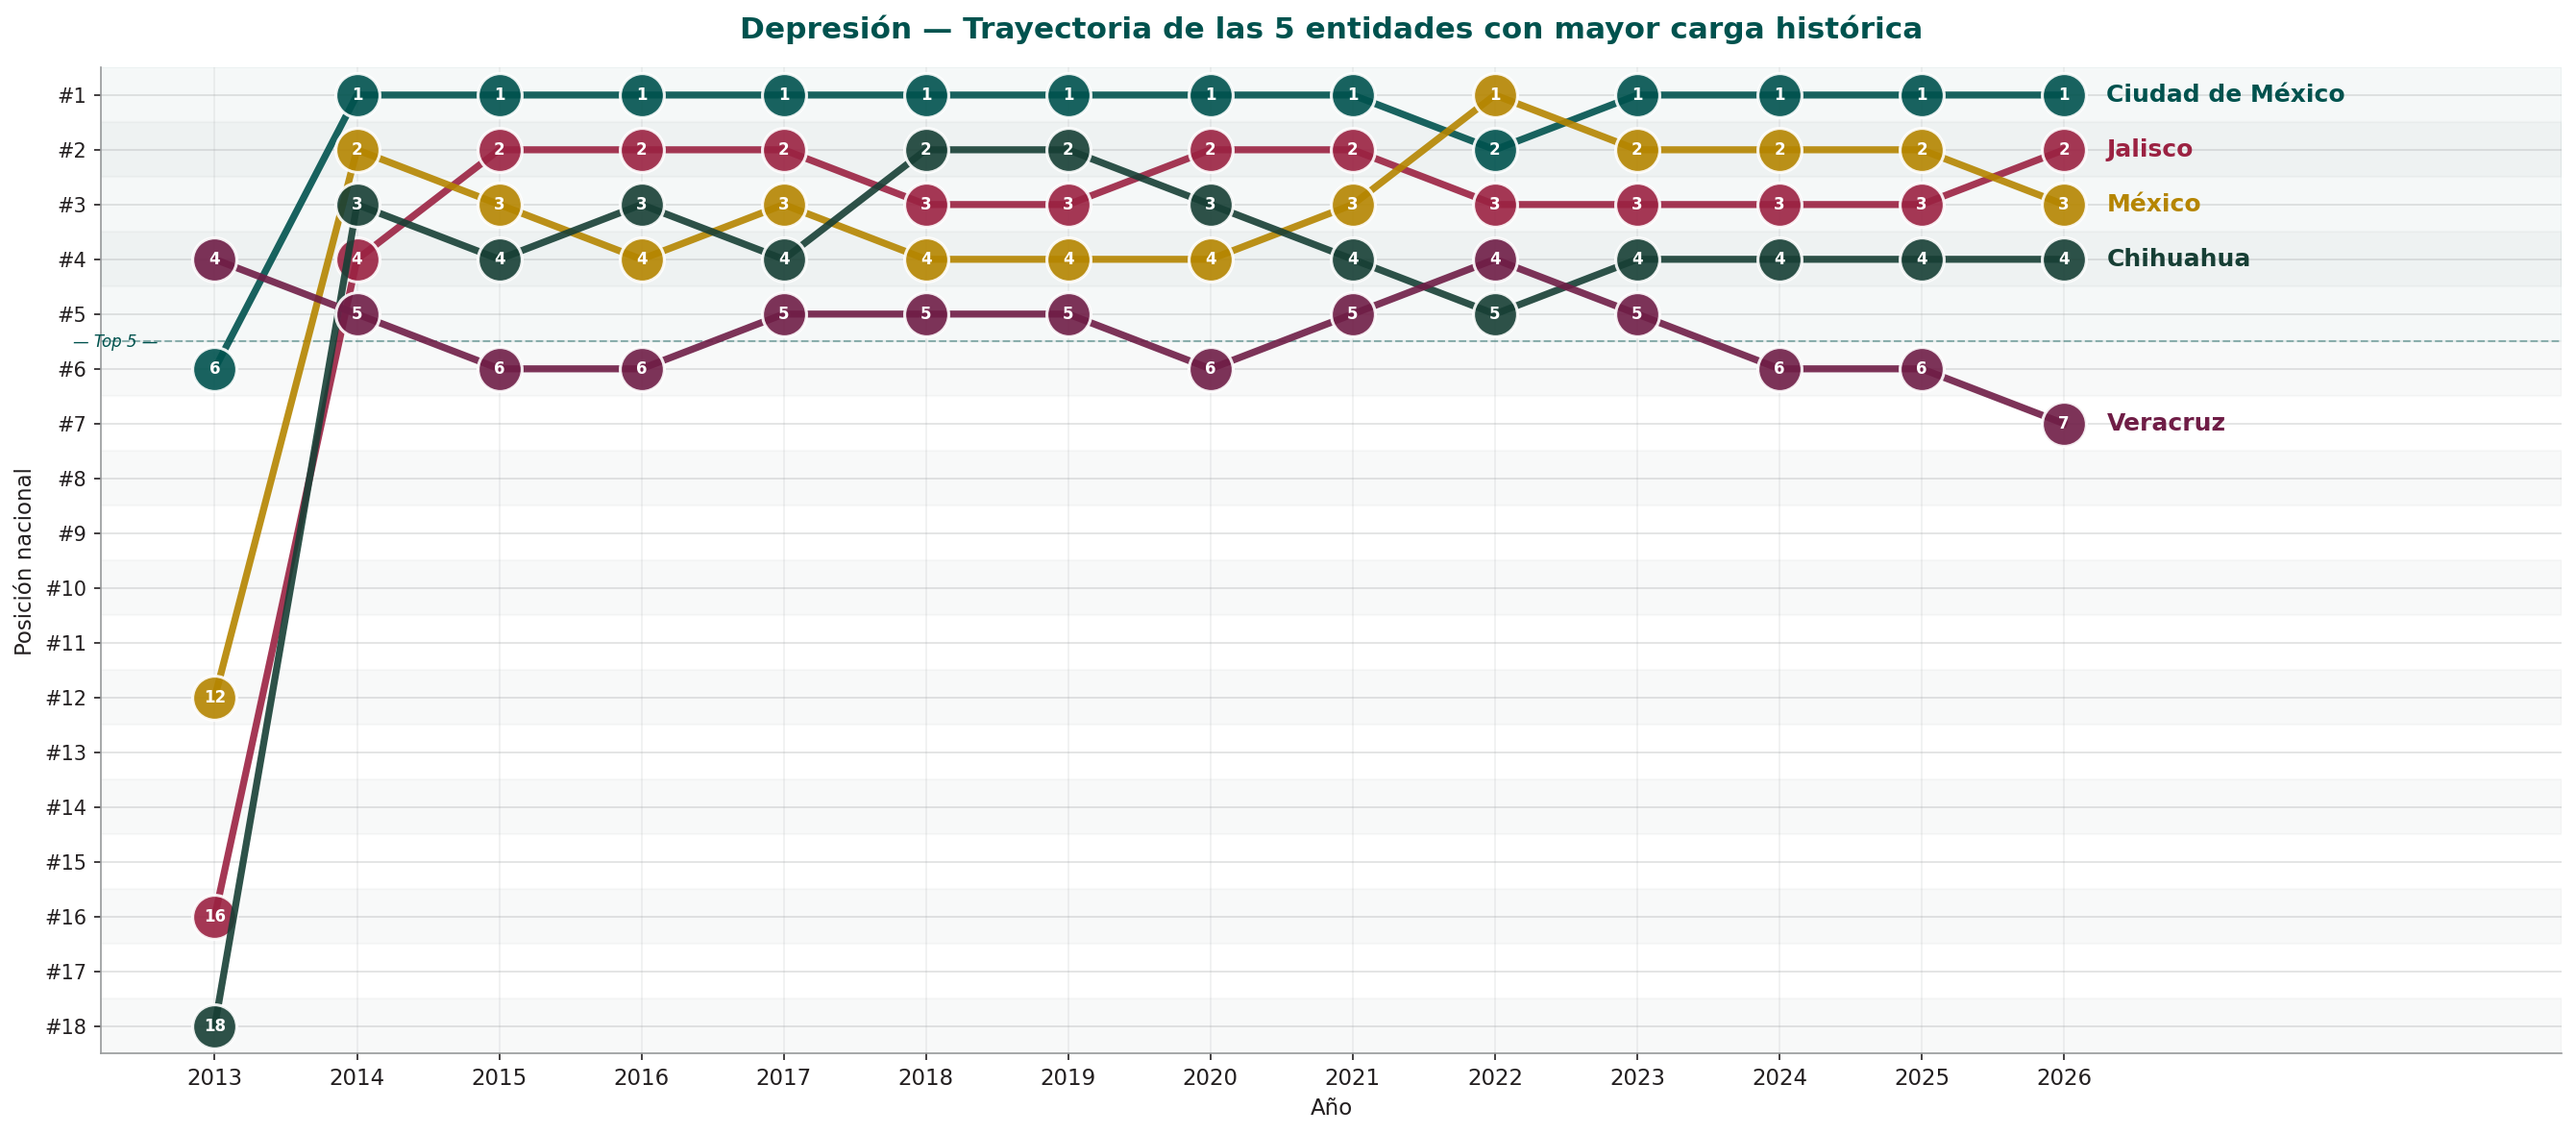
\includegraphics[width=\textwidth]{img/bump_chart_depresion.png}
    \caption{Depresión (F32) --- Trayectoria de las 5 entidades con mayor carga histórica.}
\end{figure}

\begin{figure}[H]
    \centering
    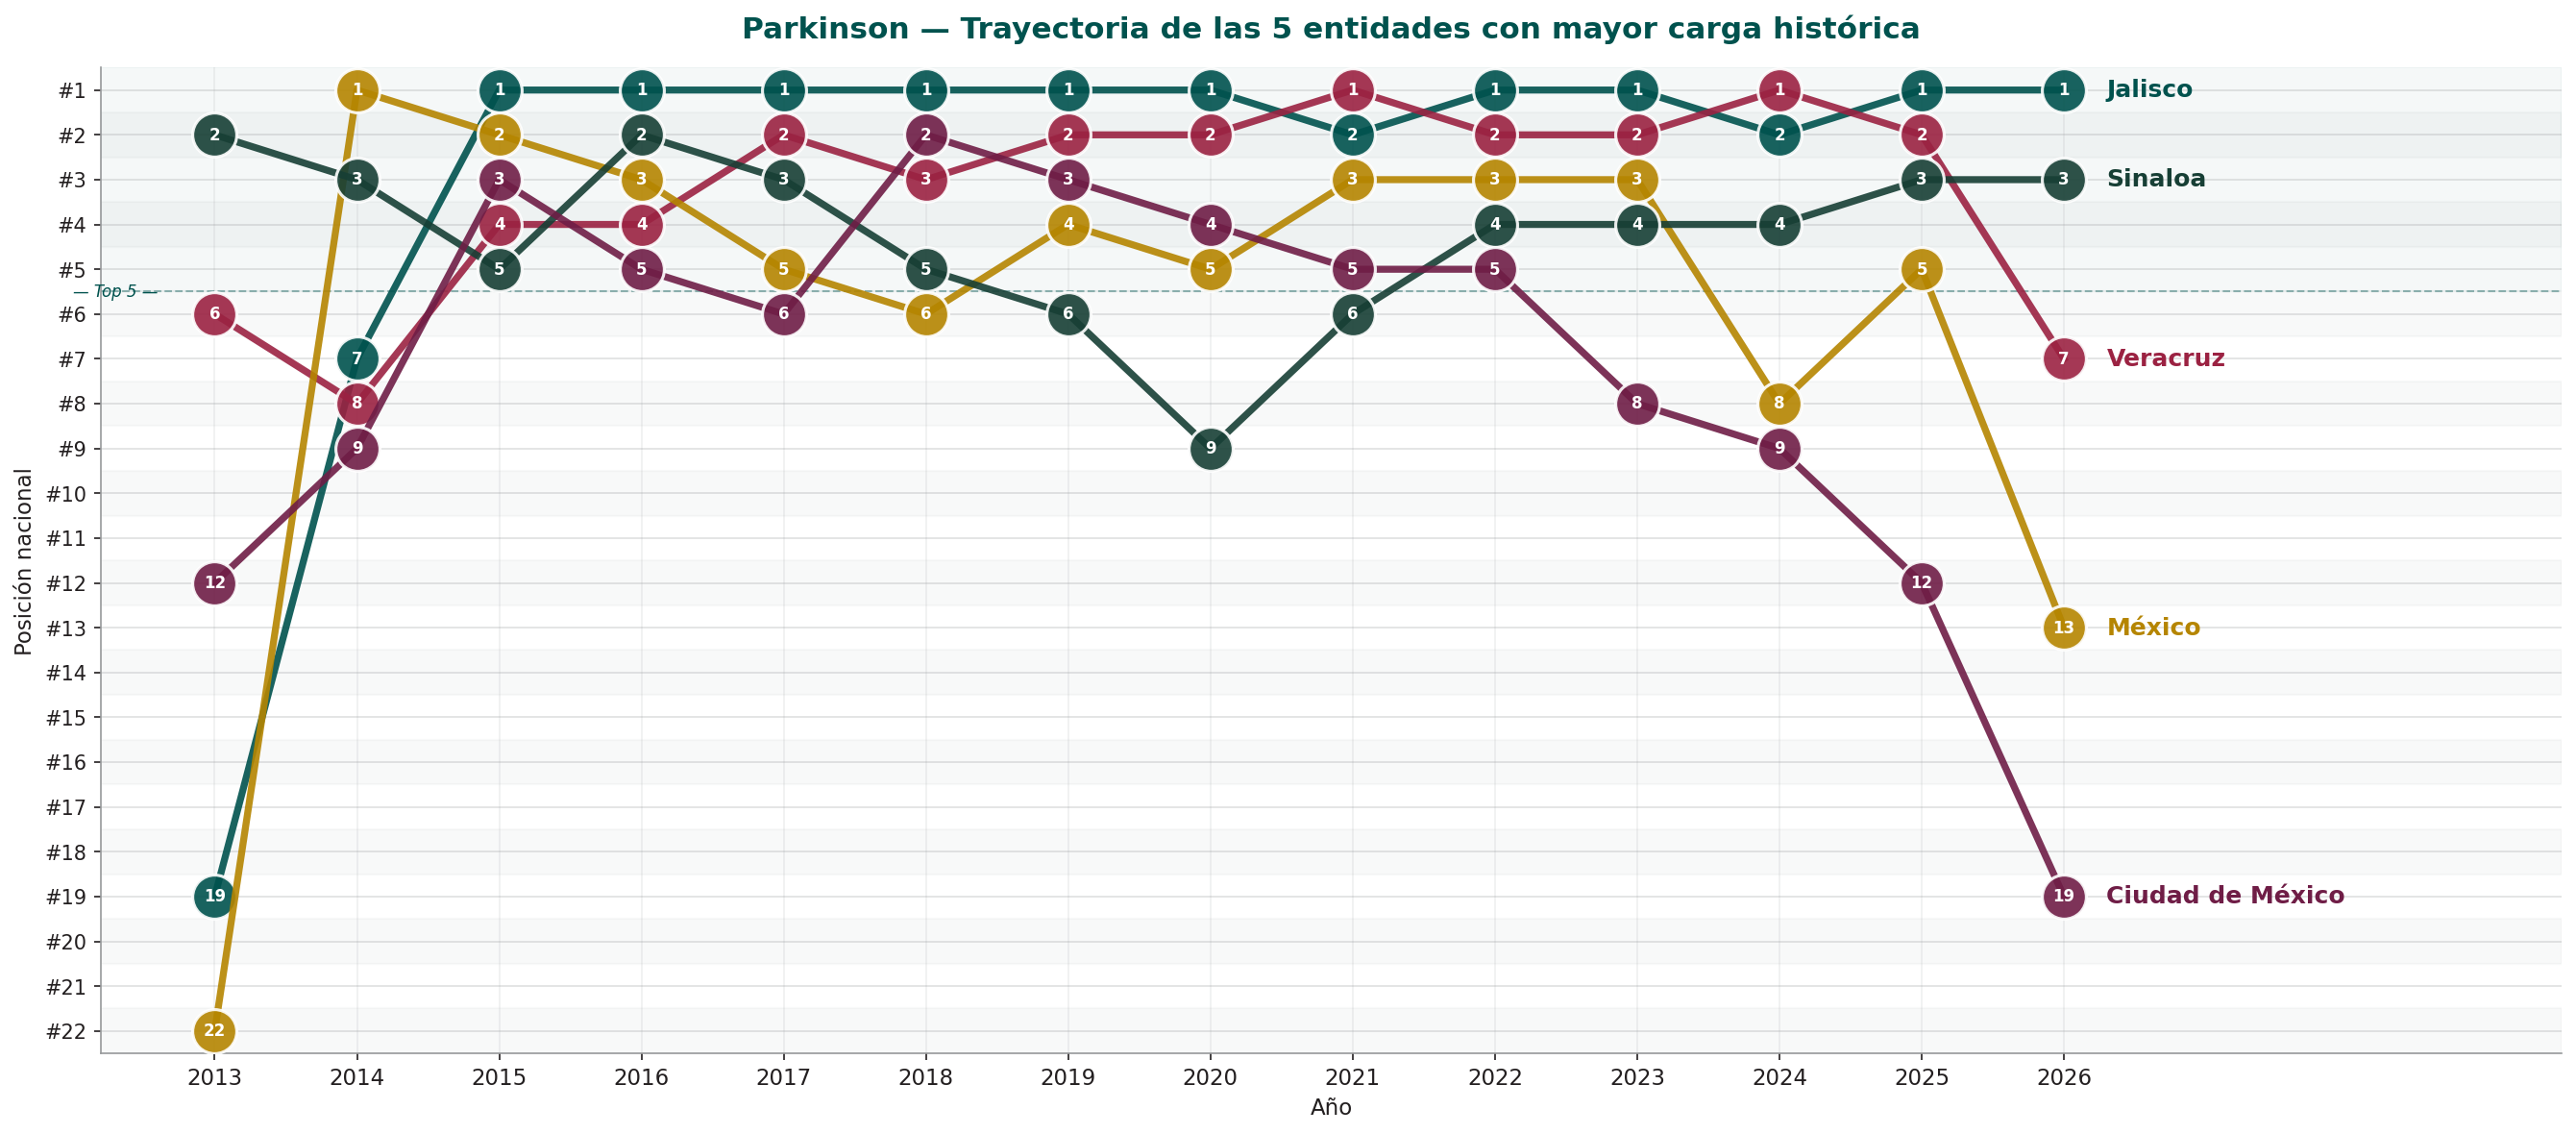
\includegraphics[width=\textwidth]{img/bump_chart_parkinson.png}
    \caption{Parkinson (G20) --- Trayectoria de las 5 entidades con mayor carga histórica.}
\end{figure}

\begin{figure}[H]
    \centering
    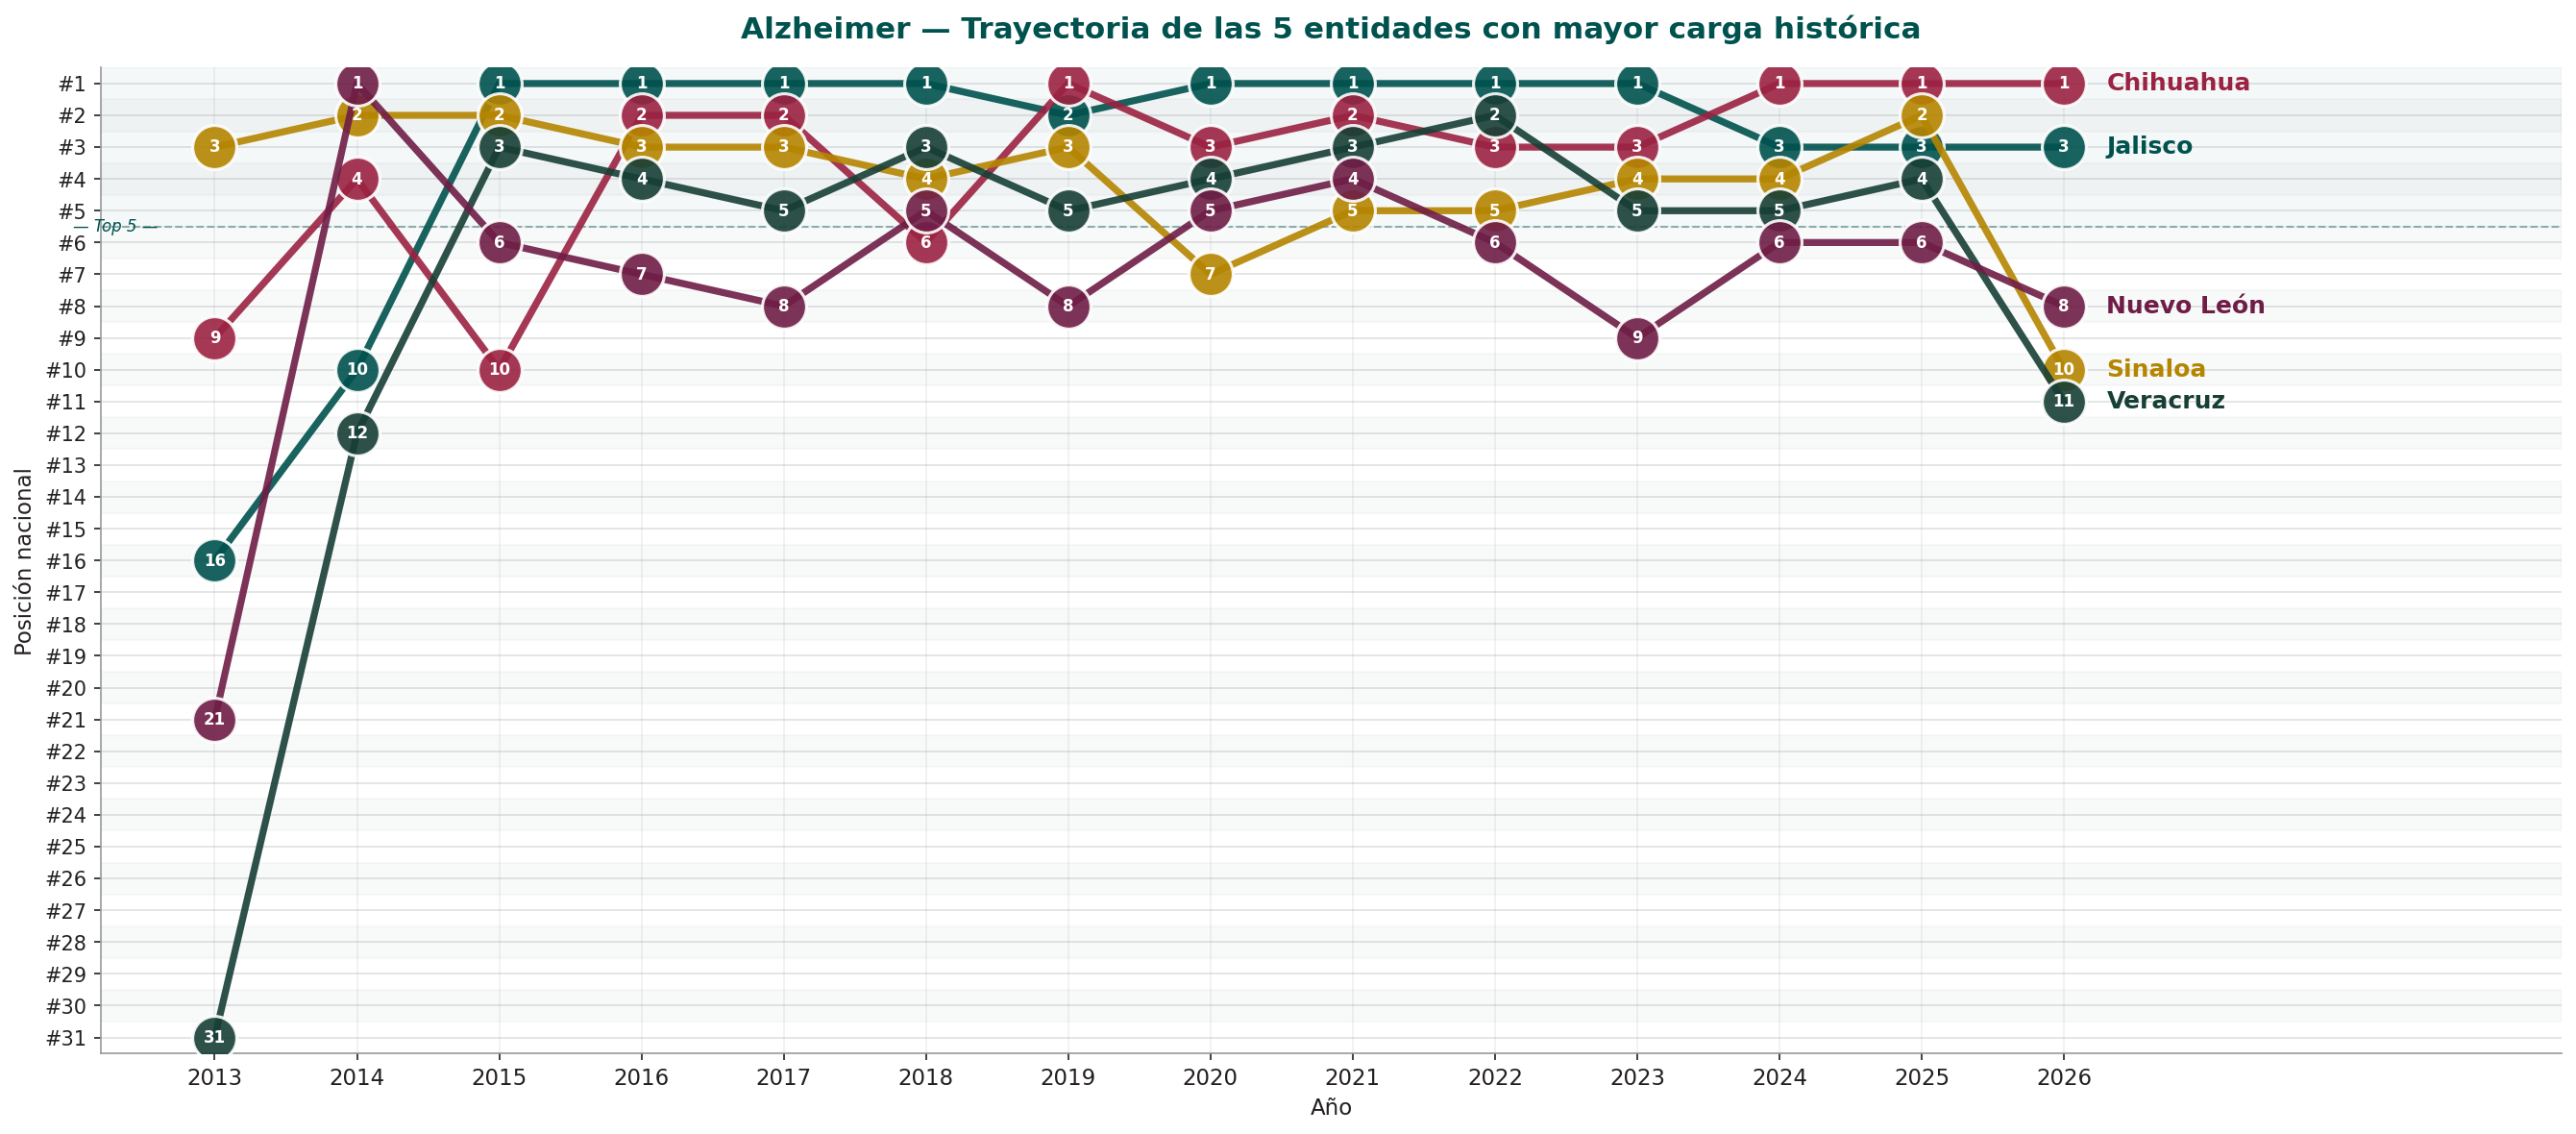
\includegraphics[width=\textwidth]{img/bump_chart_alzheimer.png}
    \caption{Alzheimer (G30) --- Trayectoria de las 5 entidades con mayor carga histórica.}
\end{figure}

% -------------------------------------------------------
\subsubsection{Impacto diferenciado del COVID-19 por entidad federativa}

Se compara la media de incrementos semanales pre-COVID (2018--2019) contra la media post-COVID (2022--2023) para cada entidad. La diferencia porcentual revela qué estados experimentaron una mayor caída sostenida o una recuperación más acelerada tras la pandemia.

\begin{figure}[H]
    \centering
    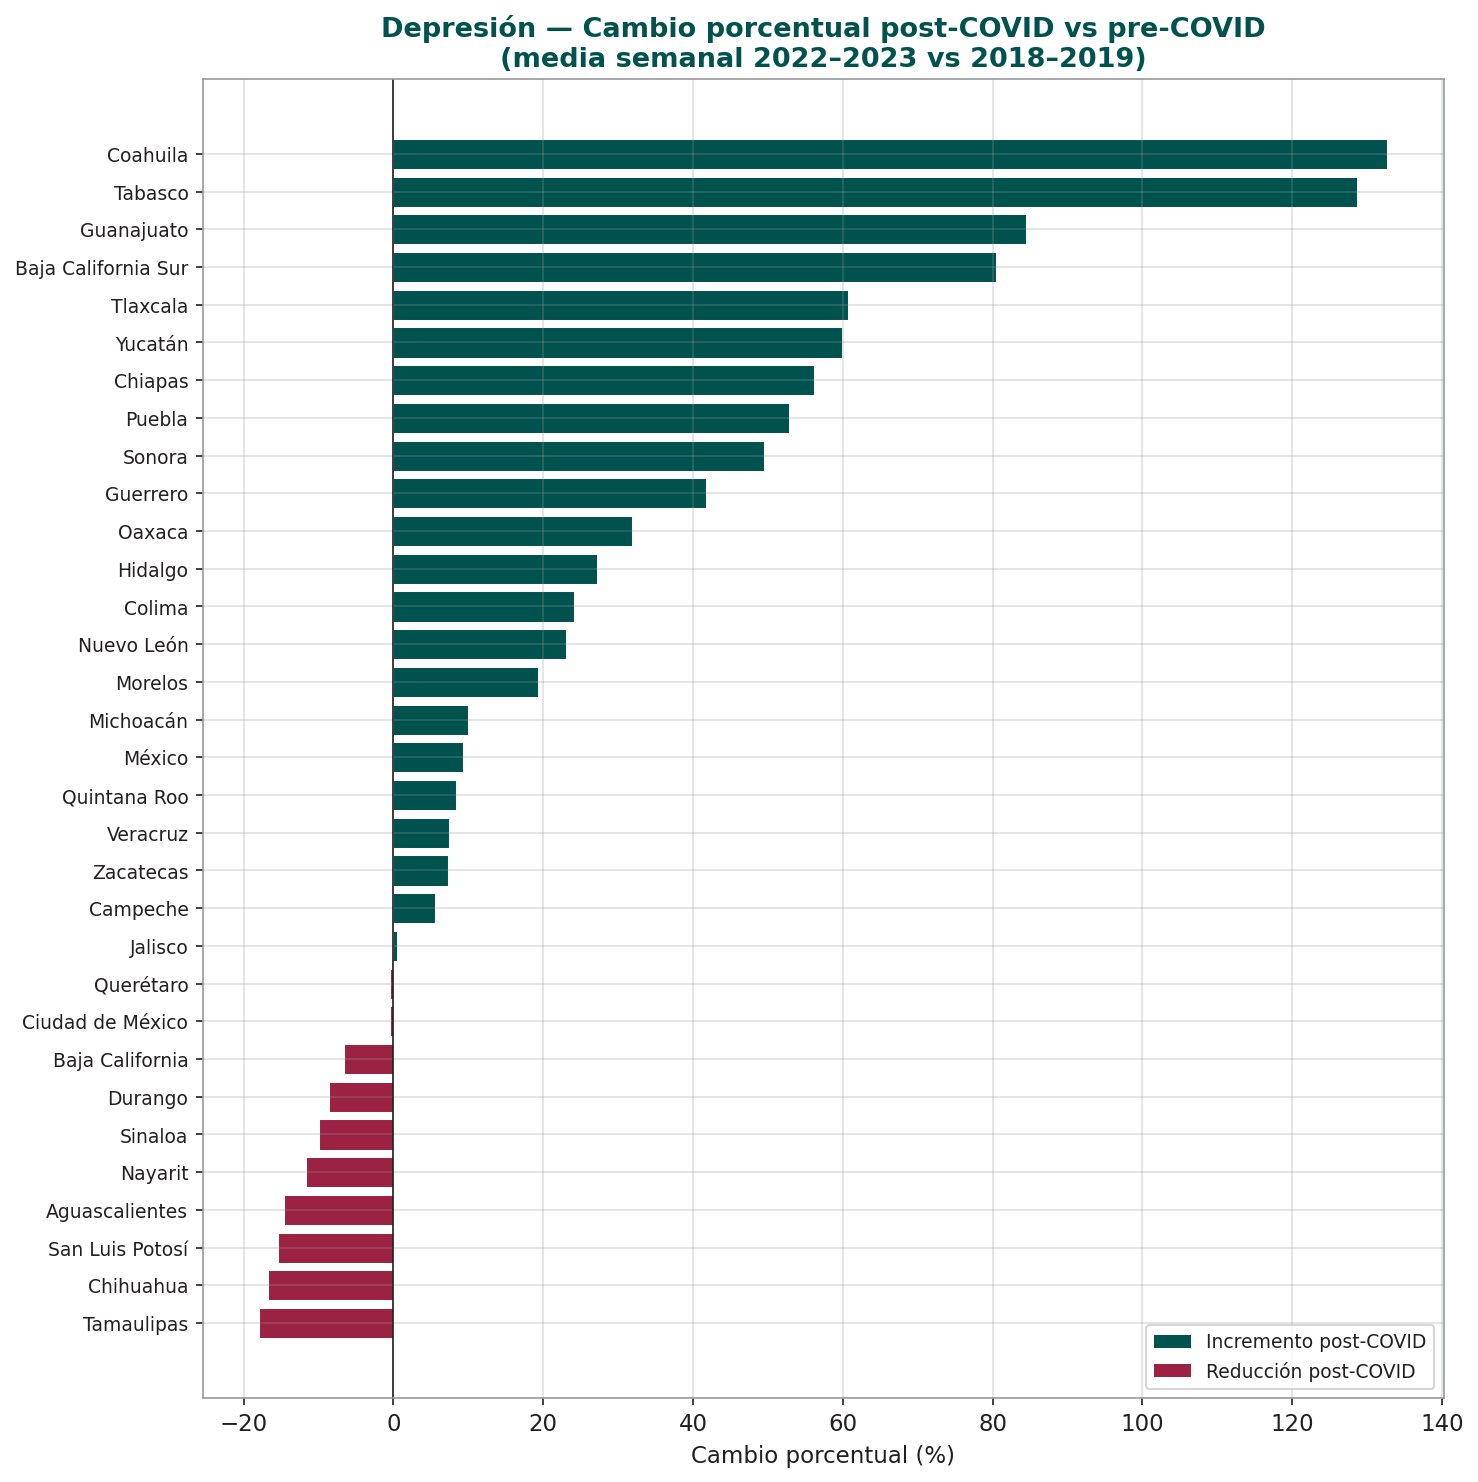
\includegraphics[width=\textwidth]{img/impacto_covid_depresion.png}
    \caption{Depresión (F32) --- Cambio porcentual post-COVID vs pre-COVID por entidad.}
\end{figure}

\begin{figure}[H]
    \centering
    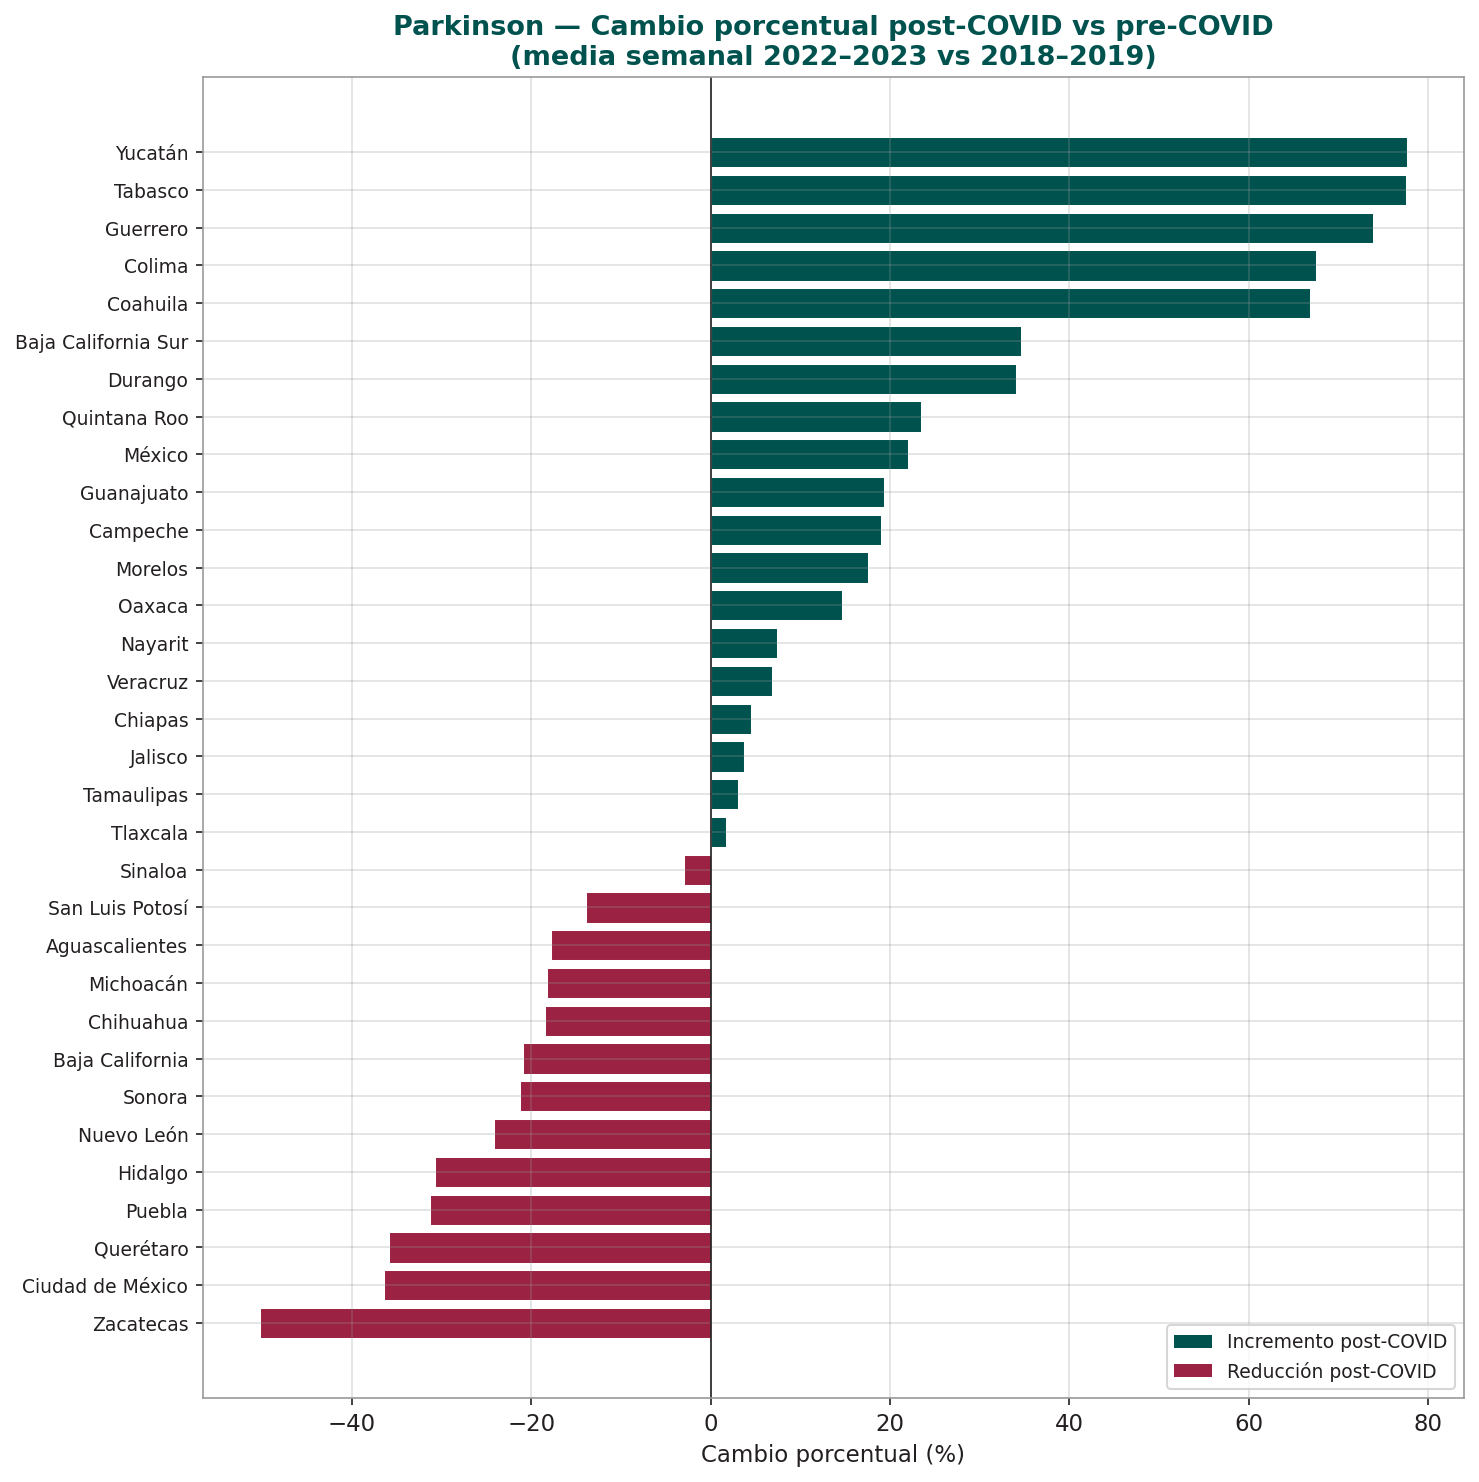
\includegraphics[width=\textwidth]{img/impacto_covid_parkinson.png}
    \caption{Parkinson (G20) --- Cambio porcentual post-COVID vs pre-COVID por entidad.}
\end{figure}

\begin{figure}[H]
    \centering
    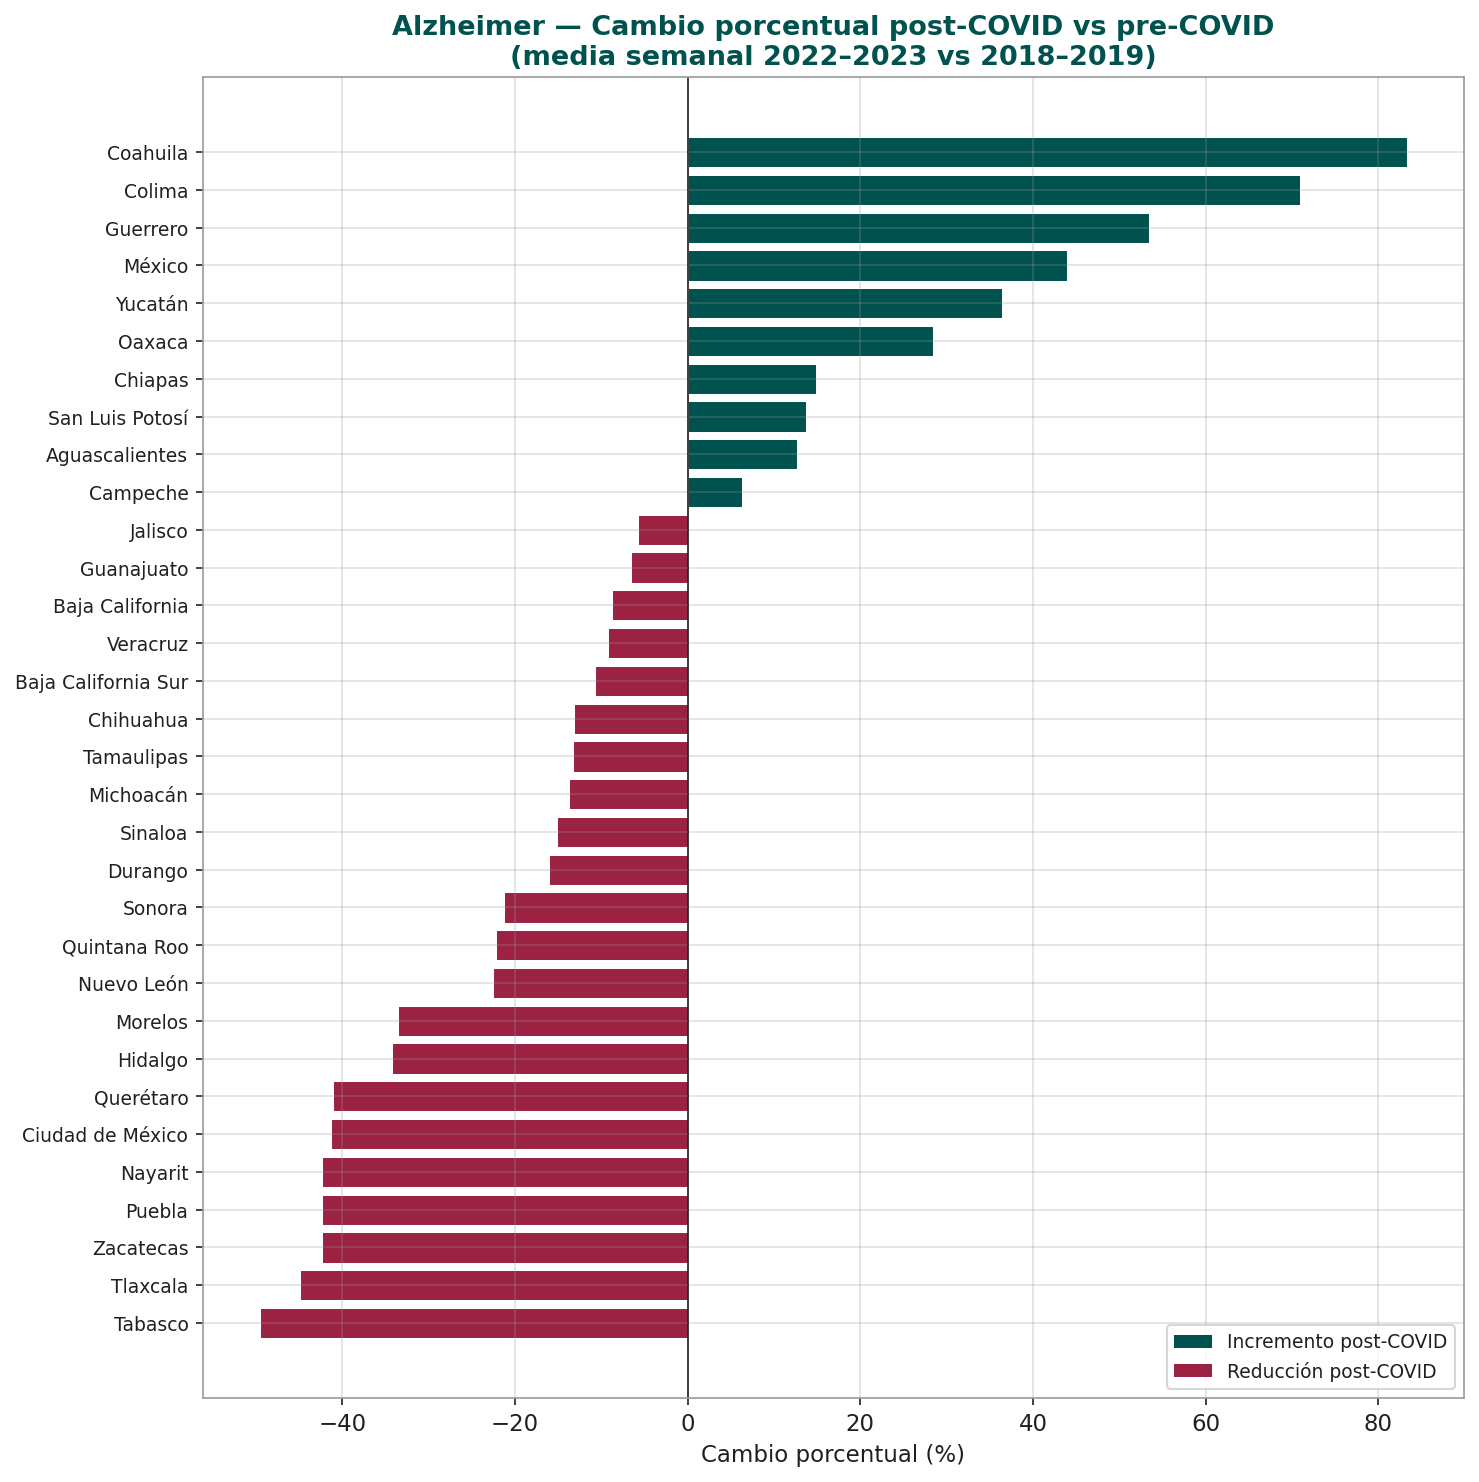
\includegraphics[width=\textwidth]{img/impacto_covid_alzheimer.png}
    \caption{Alzheimer (G30) --- Cambio porcentual post-COVID vs pre-COVID por entidad.}
\end{figure}

% -------------------------------------------------------
\subsubsection{Interpretación del análisis por entidad federativa}

\paragraph{Carga absoluta vs.\ tasa per cápita.}
El ranking por valores absolutos está dominado por las entidades más pobladas del país: Ciudad de México, Estado de México, Jalisco y Nuevo León concentran la mayor parte de los casos reportados. Sin embargo, al normalizar por población, entidades con menor población pero alta incidencia relativa ---como Colima, Aguascalientes, Baja California Sur o Tlaxcala--- emergen con tasas proporcionalmente elevadas, lo que sugiere factores locales (capacidad diagnóstica, cobertura del sistema de salud, perfiles demográficos) que no son capturados por el análisis agregado.

\paragraph{Heterogeneidad territorial.}
Los heatmaps revelan que la incidencia no es uniforme entre entidades ni entre años. Se observan: (a)~estados con crecimiento sostenido a lo largo de toda la serie, (b)~entidades cuyo reporte cayó abruptamente durante la pandemia y no se ha recuperado completamente, y (c)~estados con picos aislados que podrían corresponder a campañas de diagnóstico o cambios en protocolos de notificación.

\paragraph{Brecha de género a nivel estatal.}
La desagregación por sexo revela que la brecha hombres/mujeres no es uniforme entre entidades. En Depresión, la proporción de mujeres es consistentemente mayor en todas las entidades; en Parkinson y Alzheimer, ciertas entidades muestran proporciones más equilibradas o incluso invertidas, lo que podría reflejar diferencias en acceso al diagnóstico o en la composición demográfica local.

\paragraph{Estabilidad del ranking y movimientos post-COVID.}
Los bump charts muestran que las entidades dominantes en Depresión se han mantenido relativamente estables a lo largo de la serie, mientras que en Parkinson y Alzheimer se observan movimientos más pronunciados, particularmente tras la pandemia. Esto sugiere que el COVID-19 alteró de forma diferenciada las capacidades de diagnóstico y reporte según el tipo de condición.

\paragraph{Impacto diferenciado del COVID-19.}
La comparación pre-COVID vs post-COVID confirma que el impacto de la pandemia no fue homogéneo. Mientras que algunas entidades han superado sus niveles de reporte previos, otras ---particularmente en el Sur-Sureste--- muestran reducciones persistentes que podrían indicar deterioro en la cobertura diagnóstica.

\paragraph{Implicaciones para el modelado.}
Estos hallazgos refuerzan la decisión de adoptar un enfoque modular con desagregación por entidad federativa. Las diferencias estructurales entre estados justifican que los modelos Prophet incorporen estas variables como regresores exógenos o que se entrenen modelos diferenciados por grupos de entidades.

% --- Dashboard resumen ---
\begin{figure}[H]
    \centering
    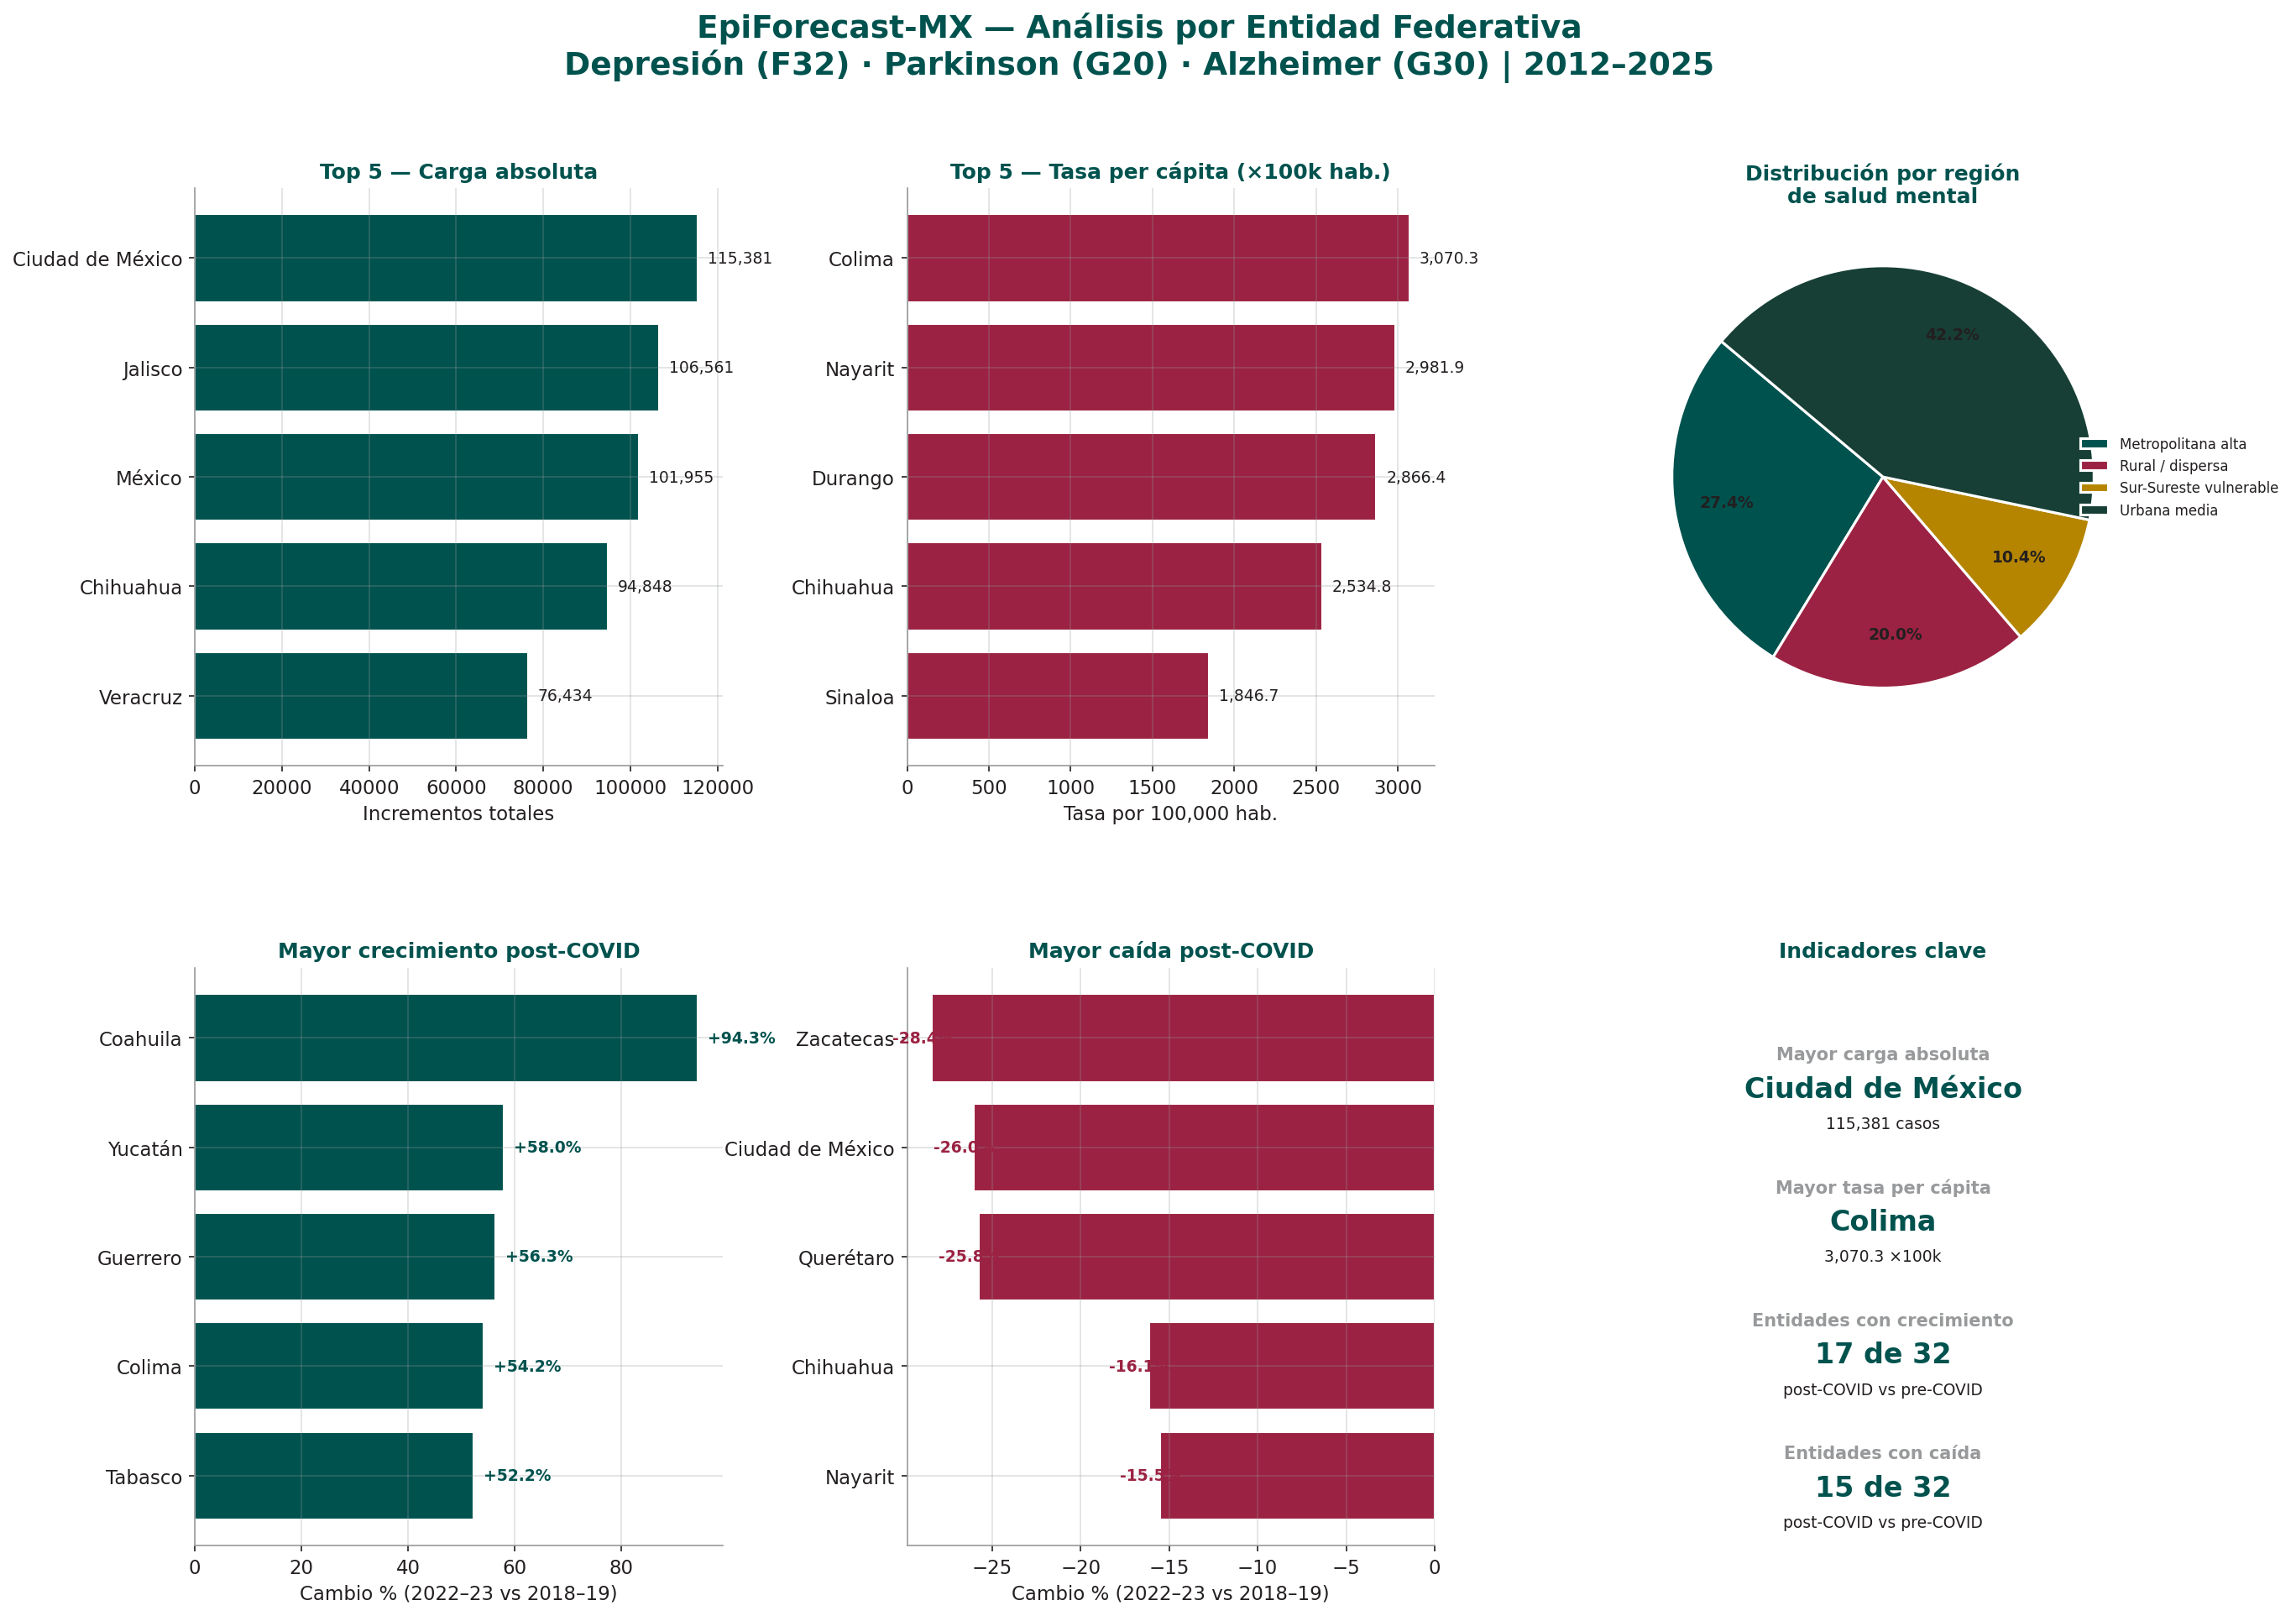
\includegraphics[width=\textwidth]{img/dashboard_analisis_entidades.png}
    \caption{Dashboard resumen del análisis por entidad federativa: carga absoluta, tasa per cápita, distribución regional, impacto COVID e indicadores clave.}
\end{figure}



\newpage

% ============================================================
% SECCIÓN 8
% ============================================================
\section{Visualización de datos}

El pipeline implementado en el proyecto \textbf{EpiForecast-MX} se mantiene consistente a lo largo de todas las etapas del análisis. Como salida de este proceso, además de los datasets en formato CSV, se genera un archivo en formato Excel (\code{.xlsx}) que sirve como fuente de datos para la capa de visualización en \textbf{Tableau}.

\subsection{Uso de Tableau Public}

Para esta etapa se creó un \textit{workbook} utilizando \textbf{Tableau Public}. Esta plataforma permite desarrollar visualizaciones interactivas y publicarlas directamente en la web. No obstante, Tableau Public presenta una limitante: no permite conectarse directamente a bases de datos ni a servicios de almacenamiento como S3. Se buscará la obtención de licencias completas de Tableau para una integración más robusta.

\subsection{Tabla de datos consolidada}

Esta vista presenta el dataset consolidado utilizado en el análisis. La tabla permite filtrar dinámicamente por año y padecimiento. Nota: la información correspondiente a 2026 es simulada y se incluye únicamente con fines informativos y exploratorios.

\begin{figure}[H]
    \centering
    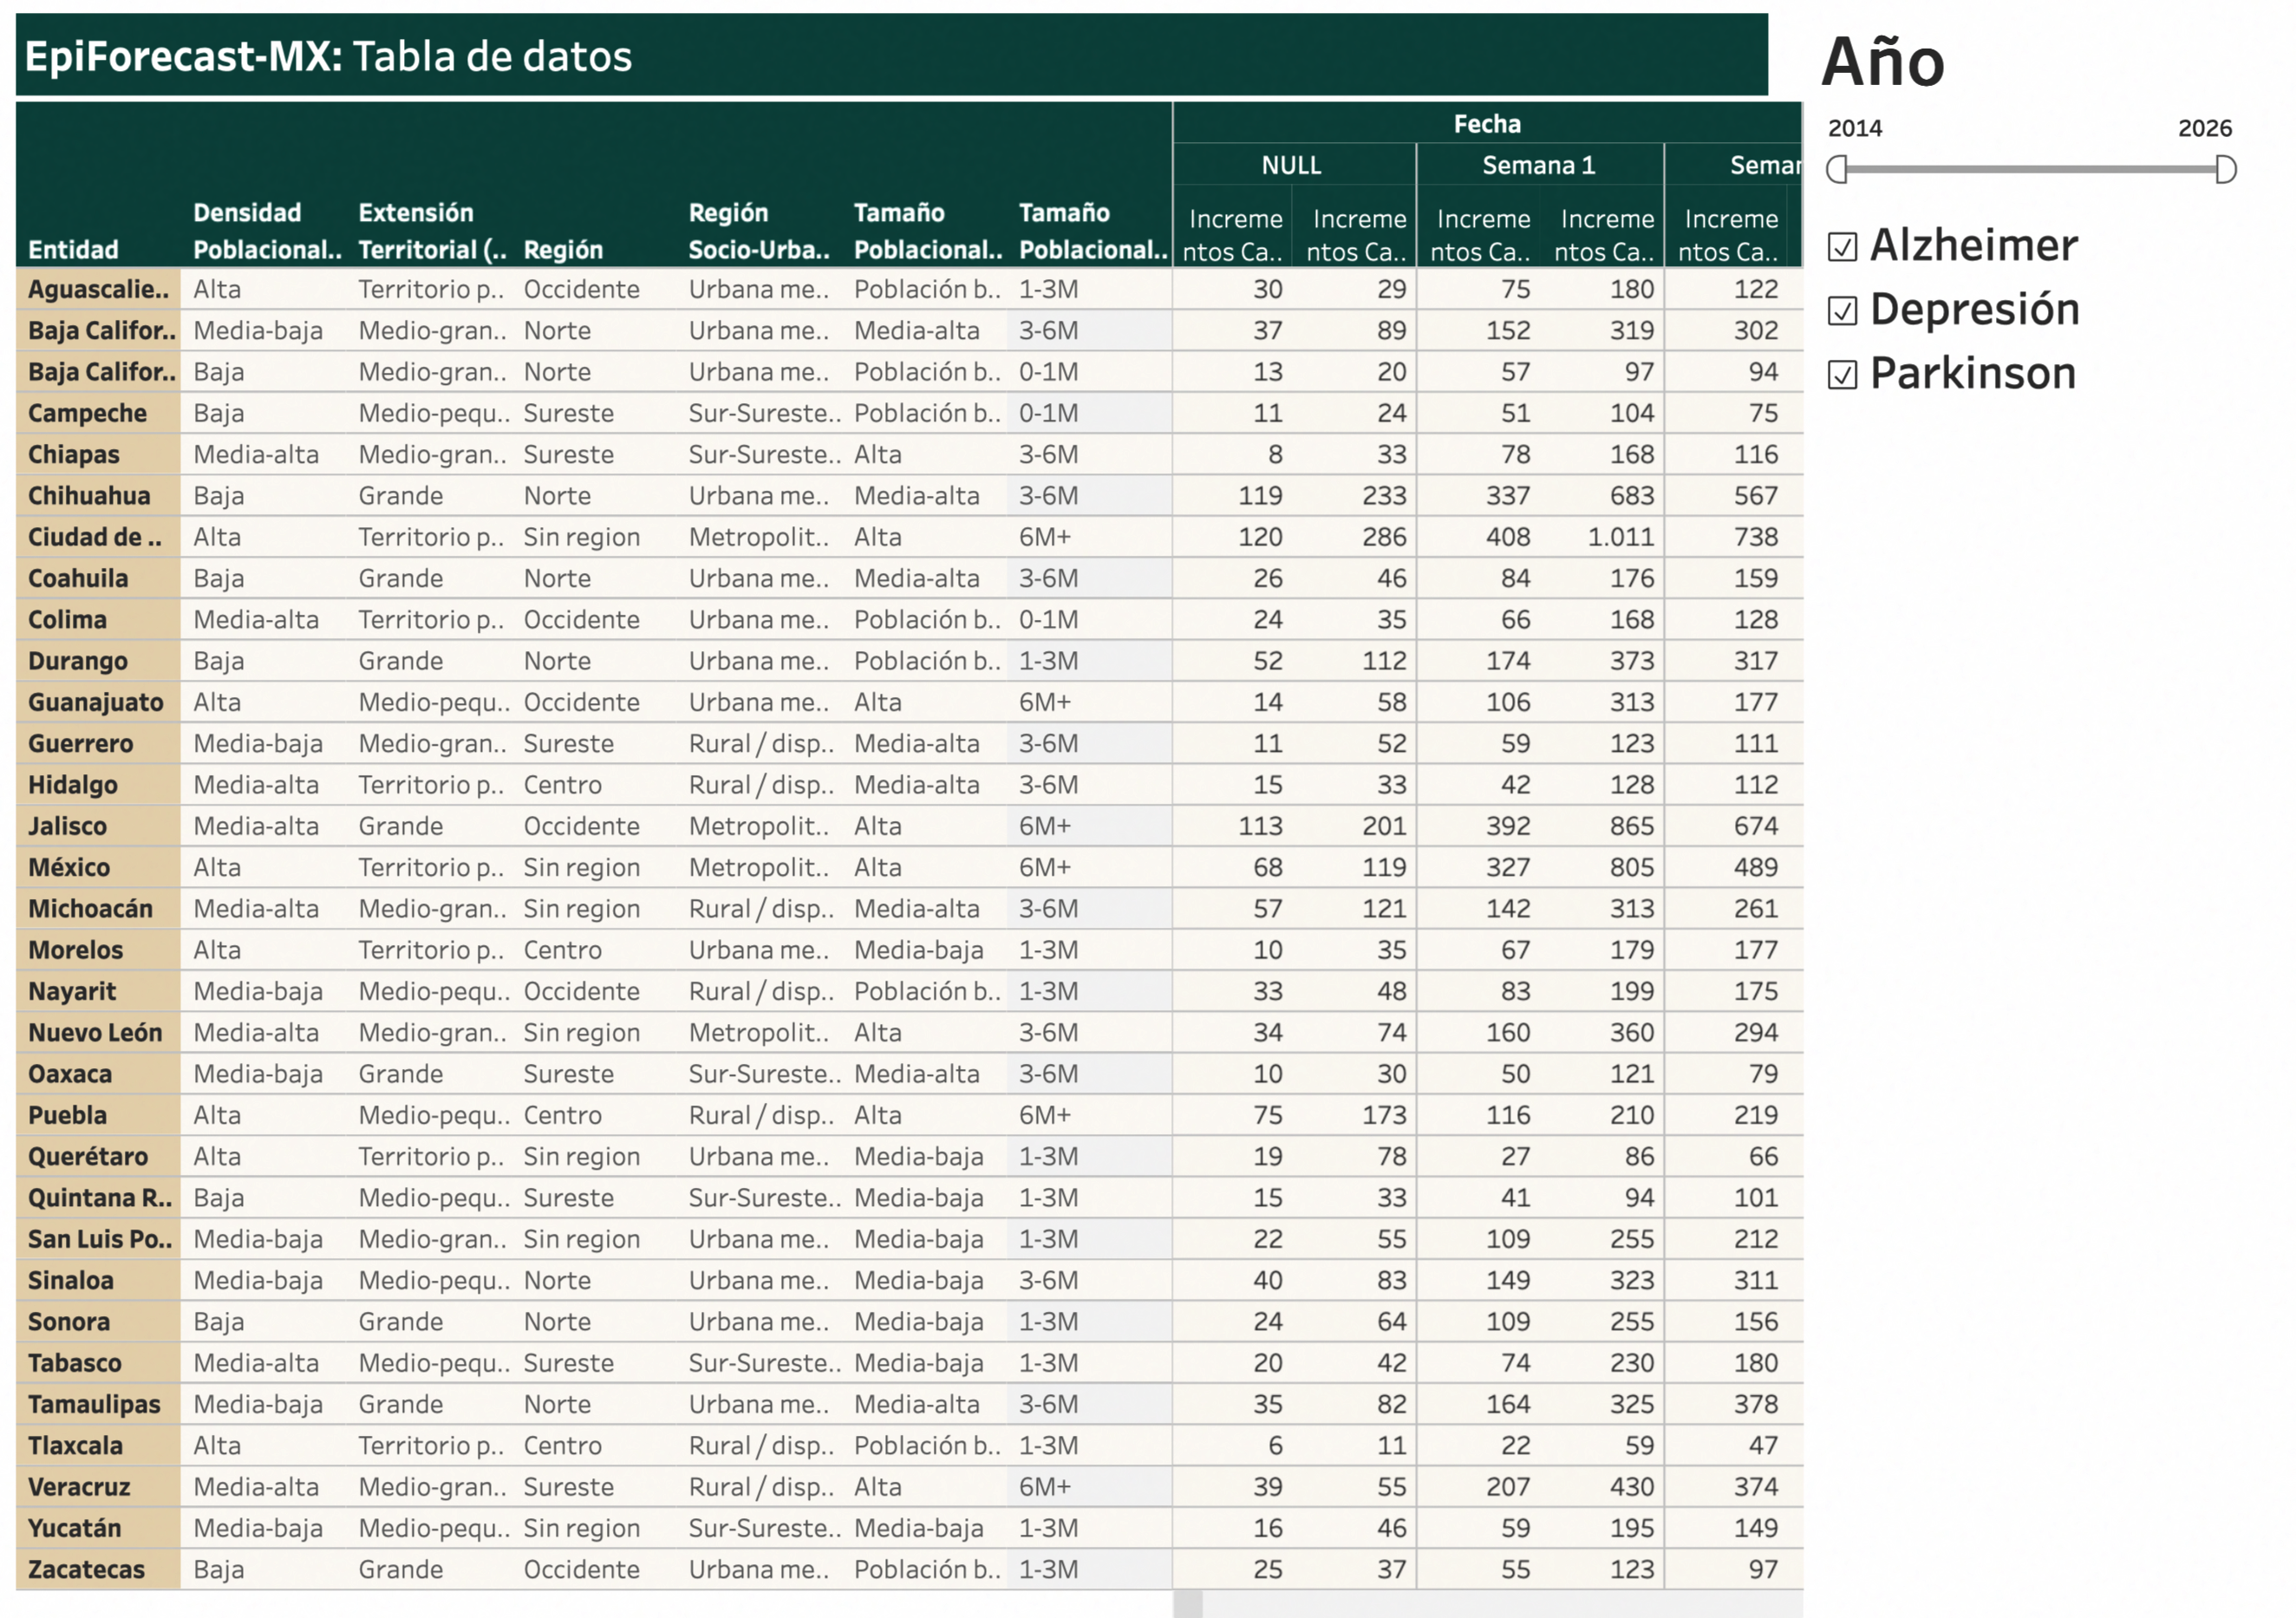
\includegraphics[width=\textwidth]{img/tableau_tabla_datos.png}
    \caption{Tabla de datos consolidada en Tableau.}
\end{figure}

\subsection{Mapa de México con variables demográficas}

Representación espacial de México a nivel de entidad federativa, incorporando variables demográficas clave provenientes de INEGI. Mediante escalas de color se visualizan indicadores como la densidad poblacional y la superficie territorial, permitiendo contrastar entidades densamente pobladas frente a territorios extensos y dispersos. Adicionalmente, el mapa integra los casos epidemiológicos desagregados por sexo.

\begin{figure}[H]
    \centering
    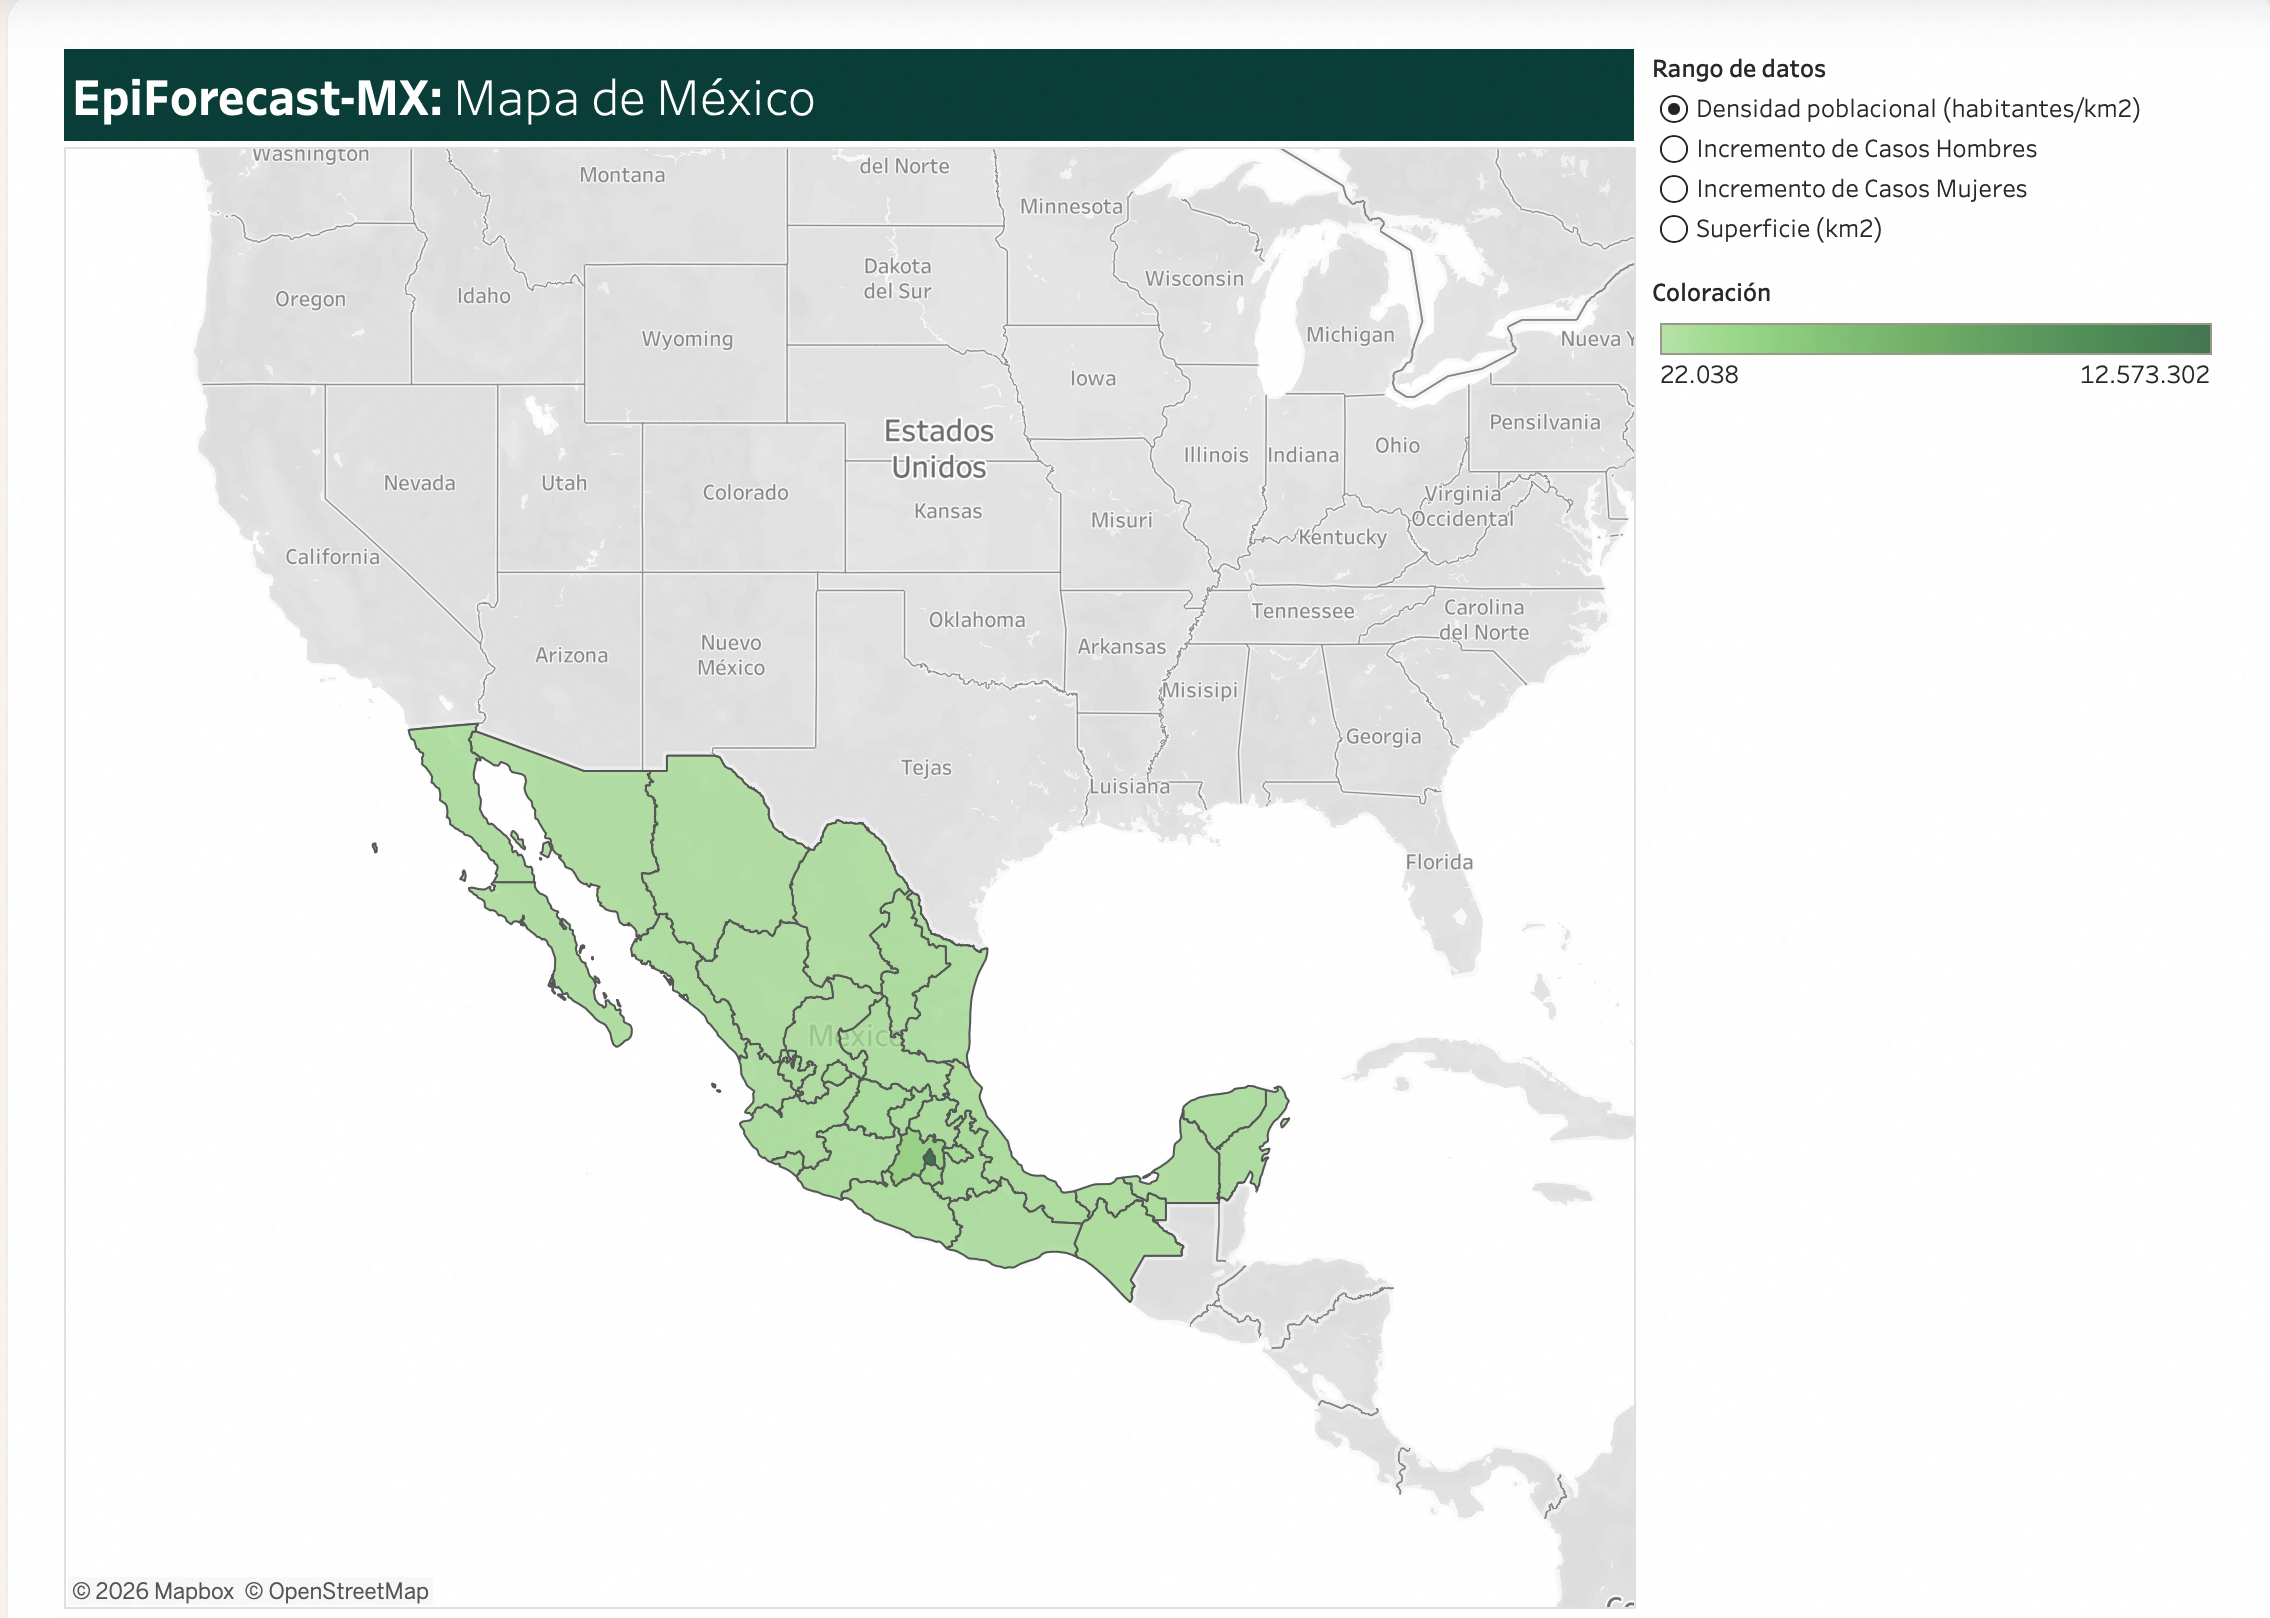
\includegraphics[width=\textwidth]{img/tableau_mapa_demografico.png}
    \caption{Mapa de México con variables demográficas.}
\end{figure}

\subsection{México en categorías}

Mapa categórico del país, construido a partir de las clasificaciones territoriales y demográficas definidas durante la fase de ingeniería de características: región de salud mental, ratio H/M, extensión territorial, densidad poblacional y tamaño poblacional por rangos fijos y por percentiles.

\begin{figure}[H]
    \centering
    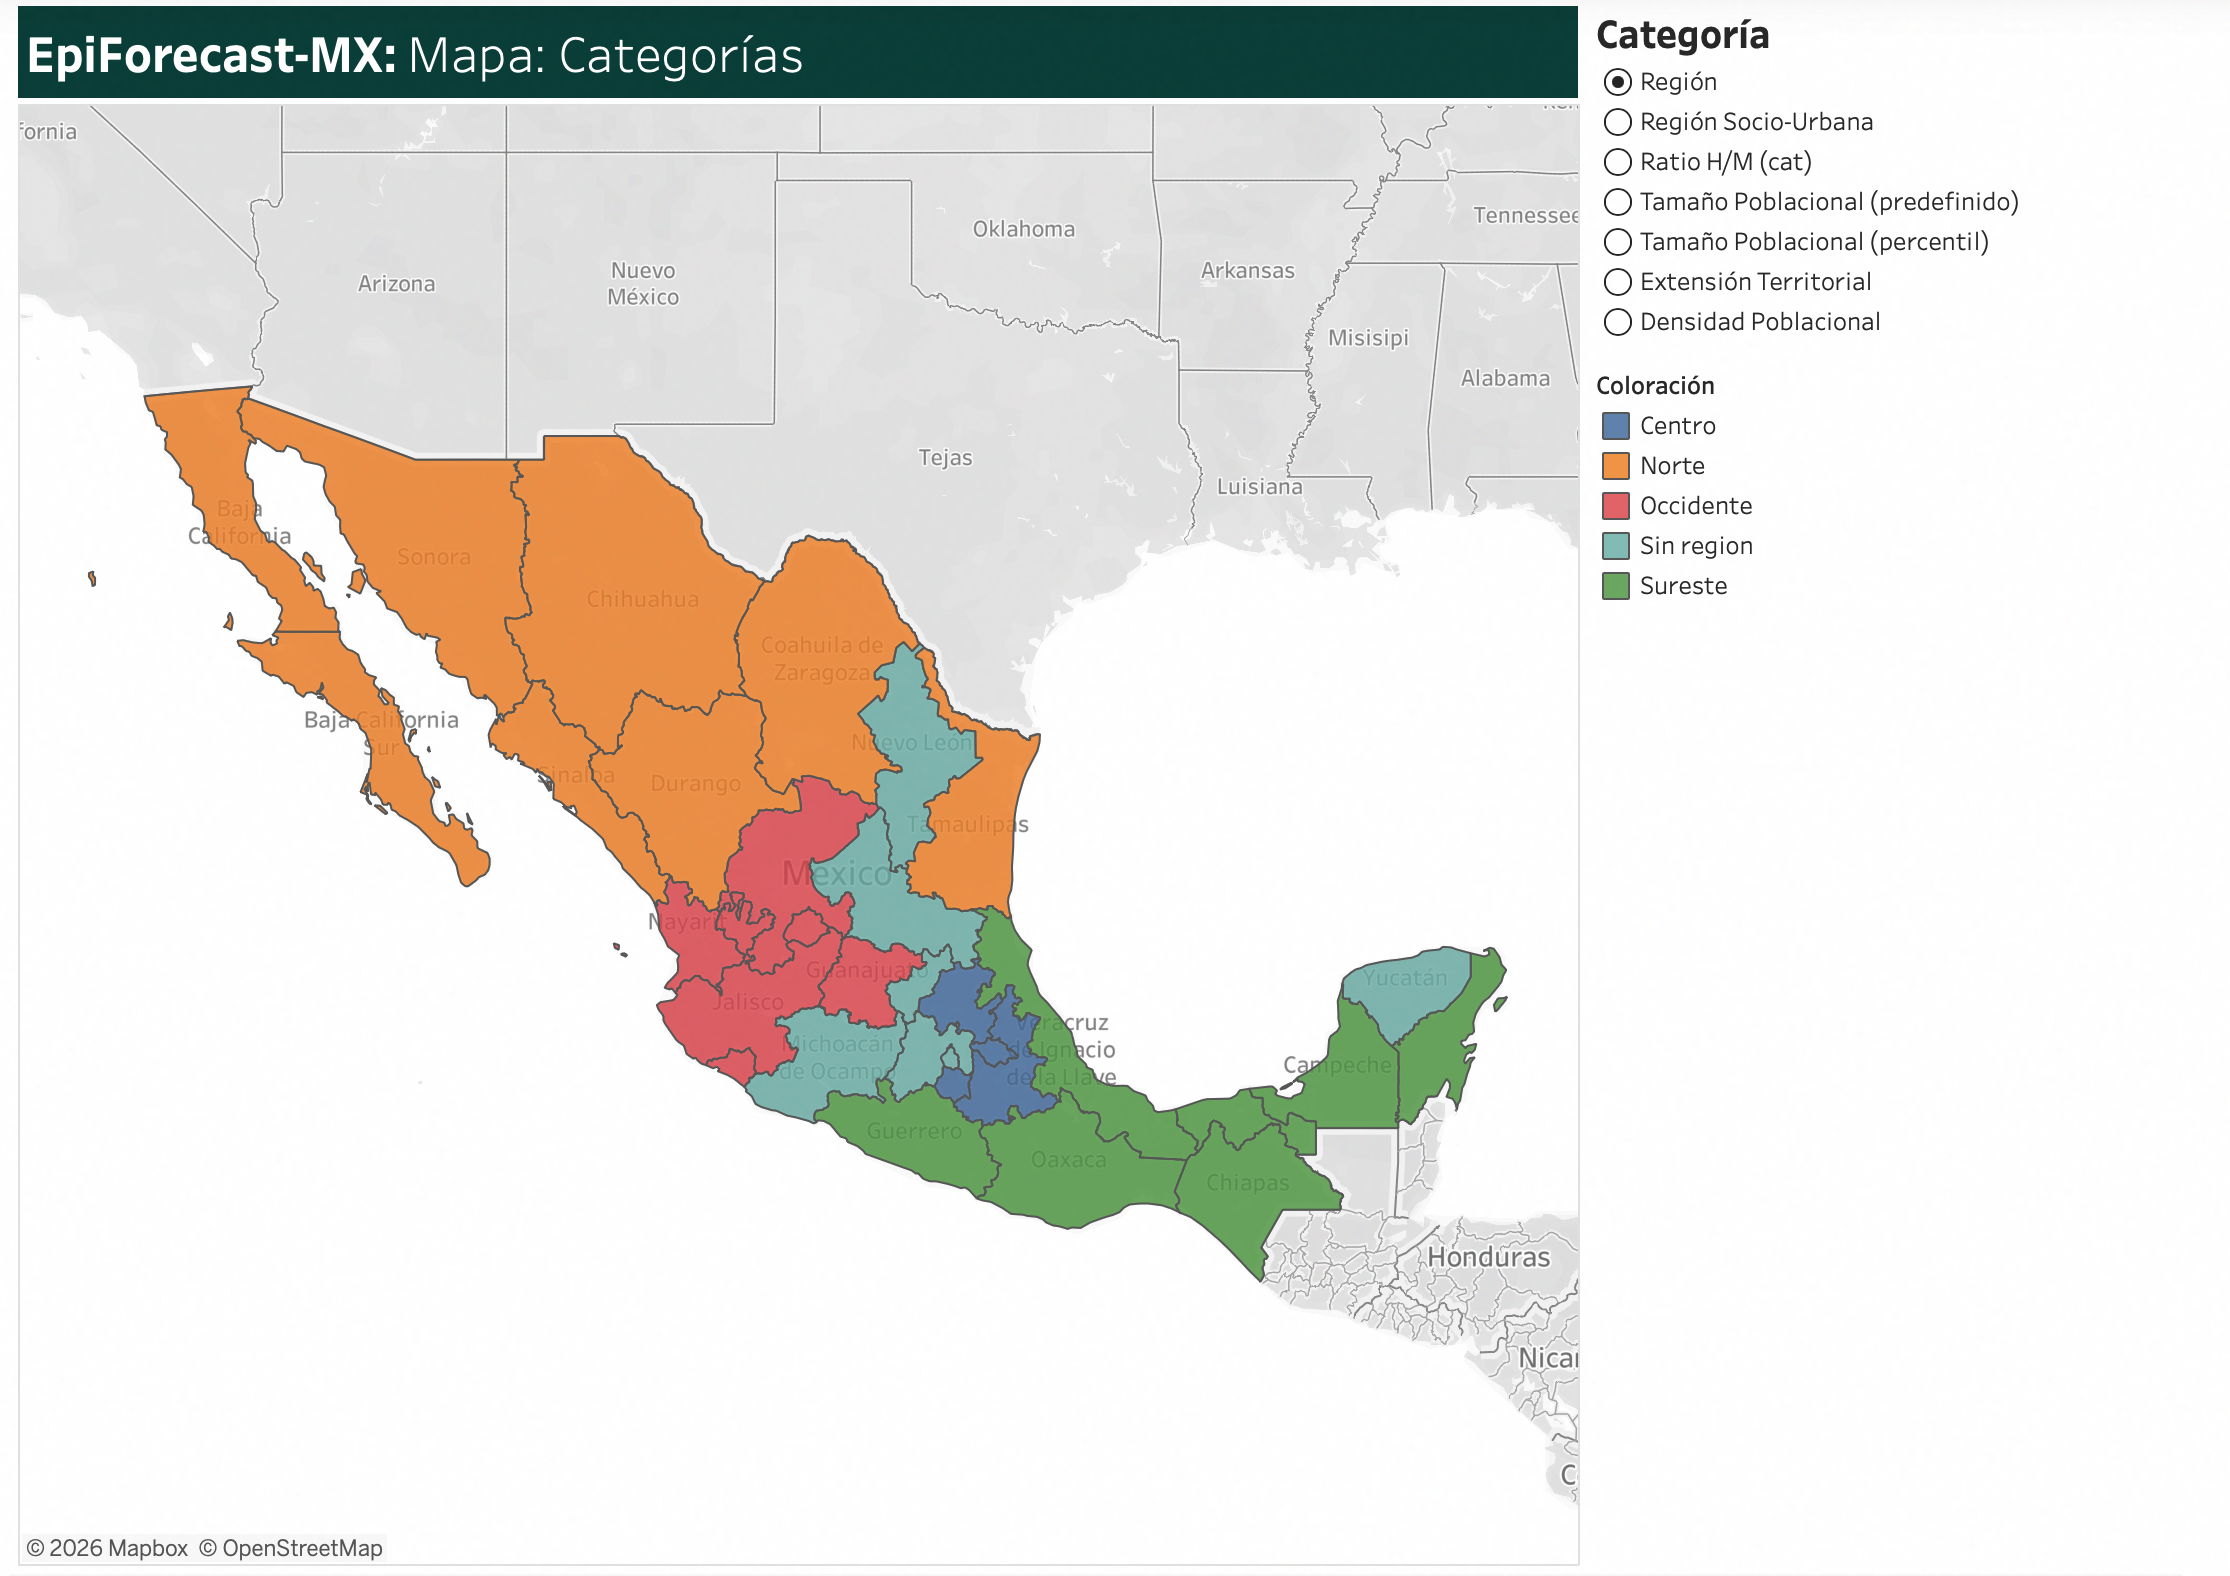
\includegraphics[width=\textwidth]{img/tableau_mapa_categorias.png}
    \caption{México en categorías territoriales y demográficas.}
\end{figure}

\subsection{Casos por año}

Incremento anual de casos, desagregado por sexo. Permite filtrar por padecimiento y comparar tendencias entre distintos años, facilitando el análisis de cambios de mediano y largo plazo.

\begin{figure}[H]
    \centering
    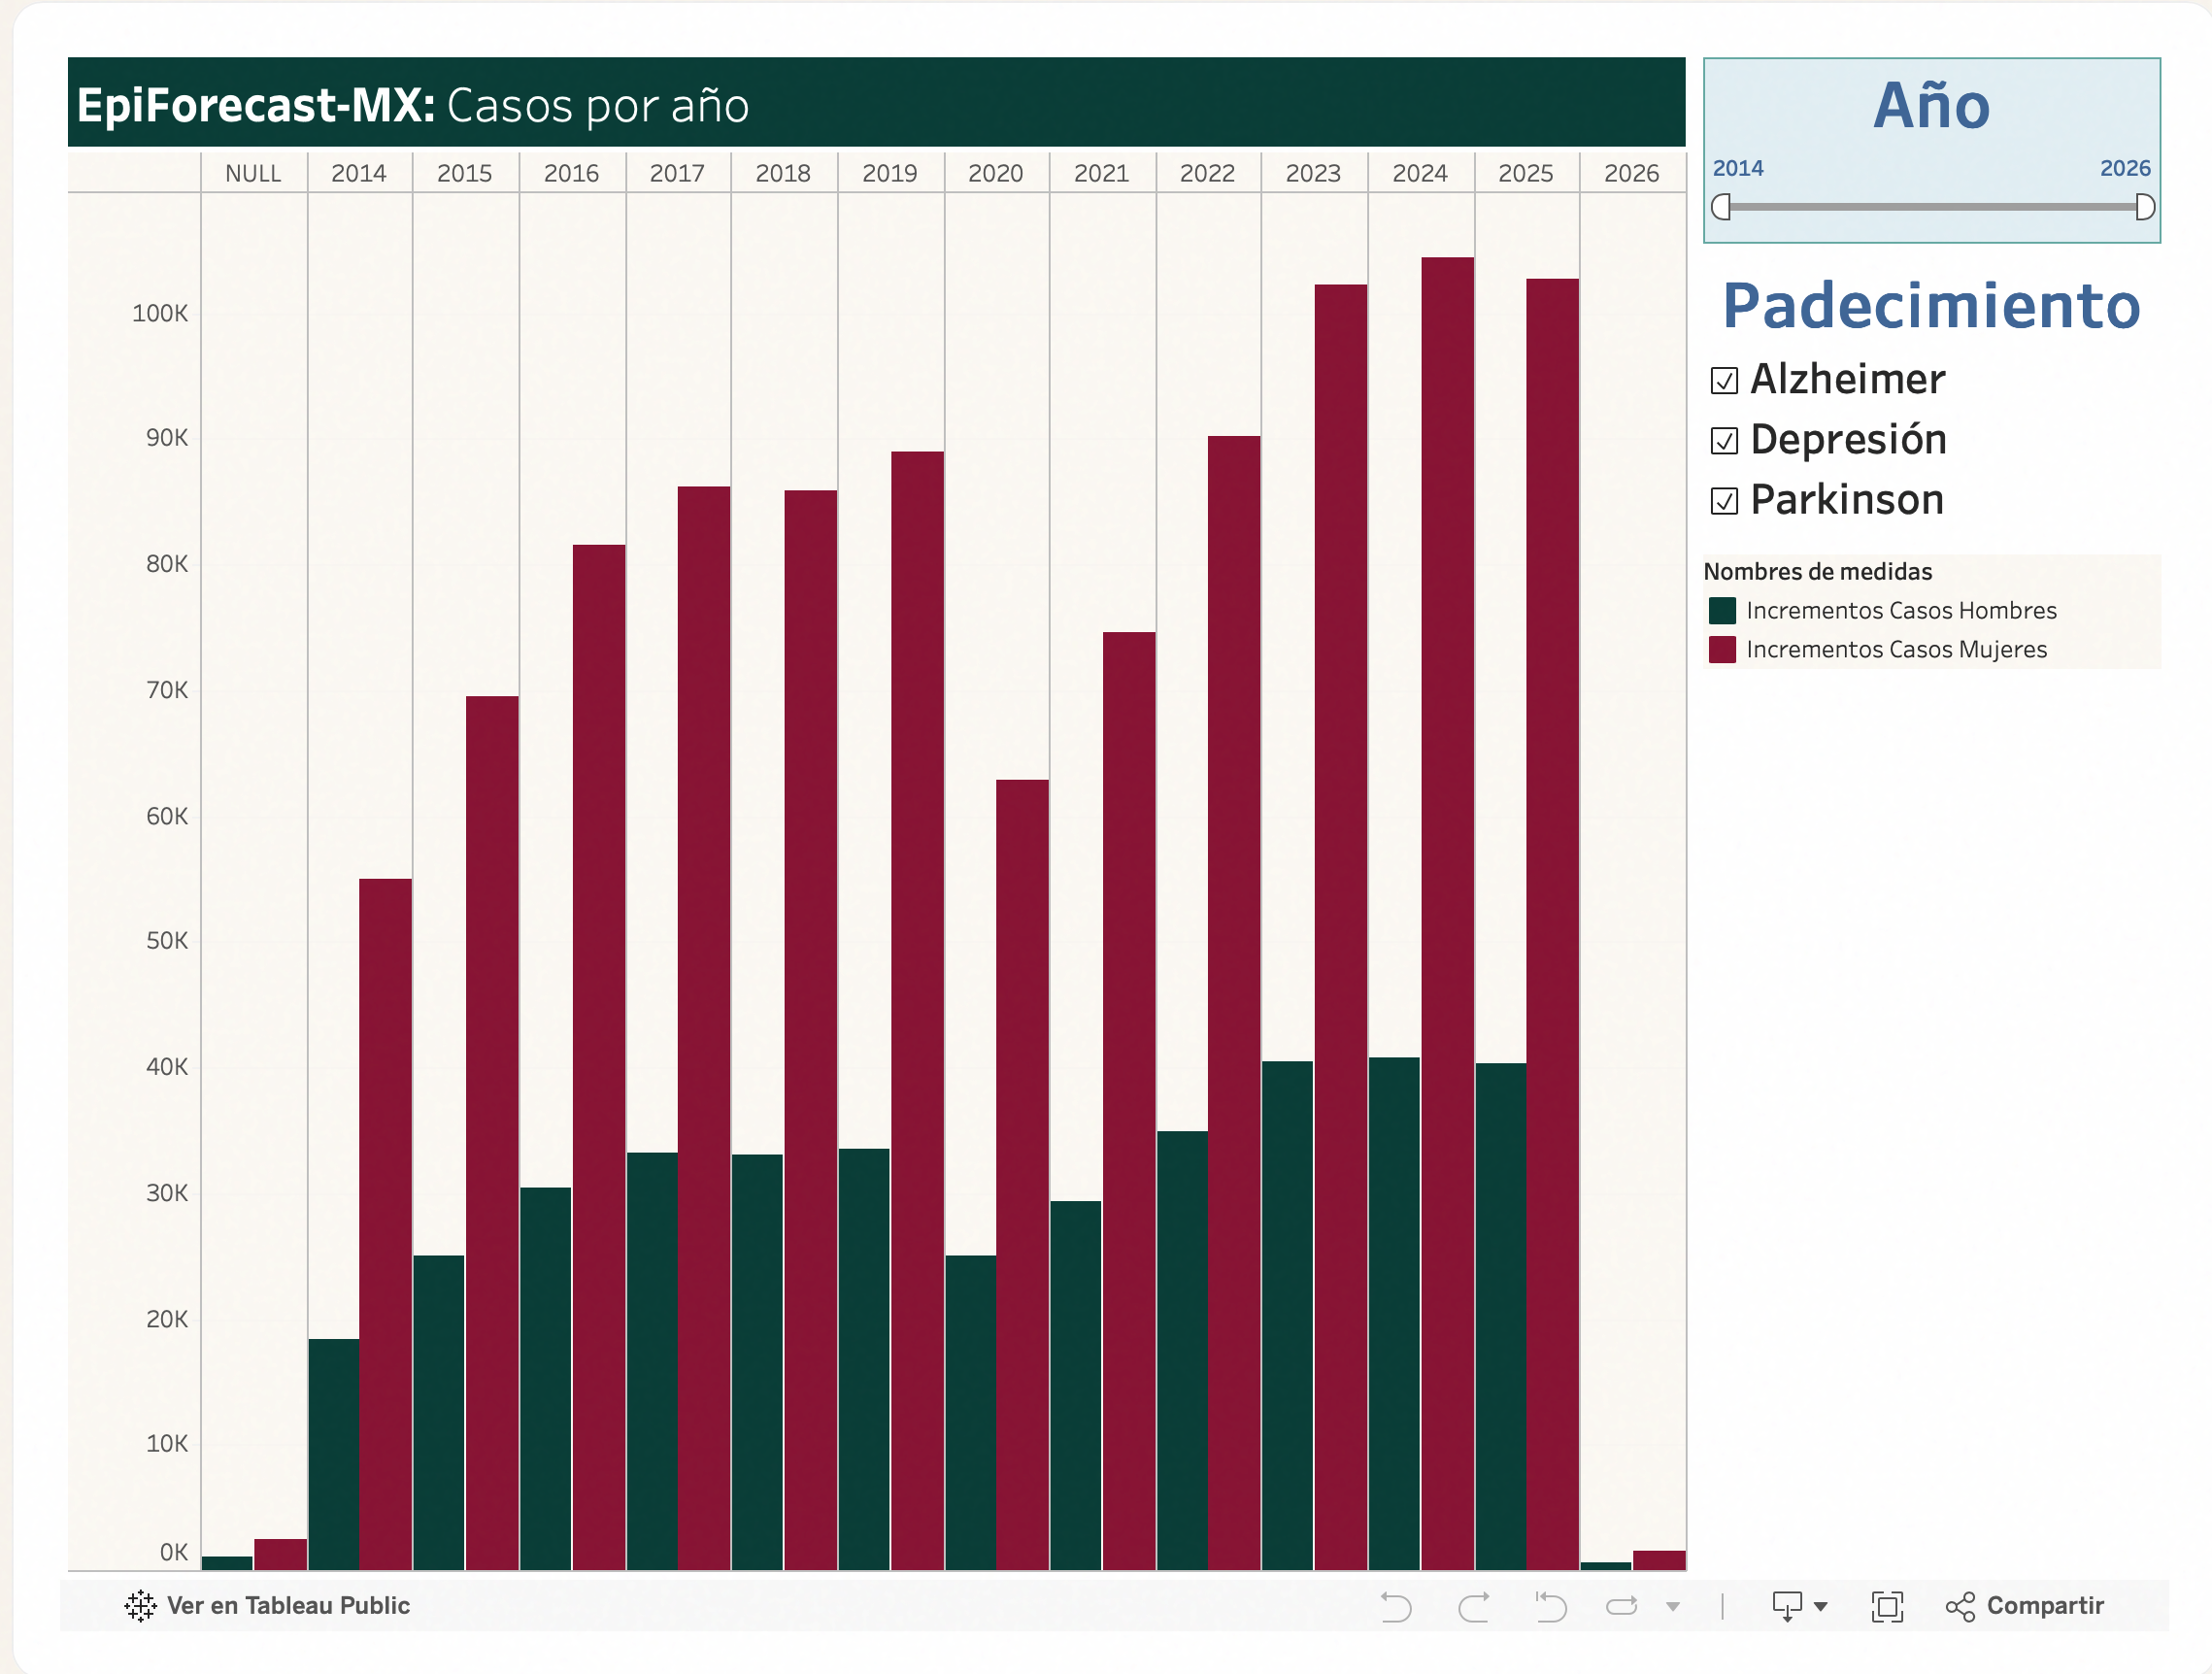
\includegraphics[width=\textwidth]{img/tableau_casos_anual.png}
    \caption{Casos por año, desagregados por sexo.}
\end{figure}

\subsection{Casos semanales}

Dinámica temporal de corto plazo, mostrando el incremento de casos semanales por sexo. La posibilidad de filtrar por año y padecimiento permite detectar variaciones intraanuales, picos, estacionalidad y cambios abruptos.

\begin{figure}[H]
    \centering
    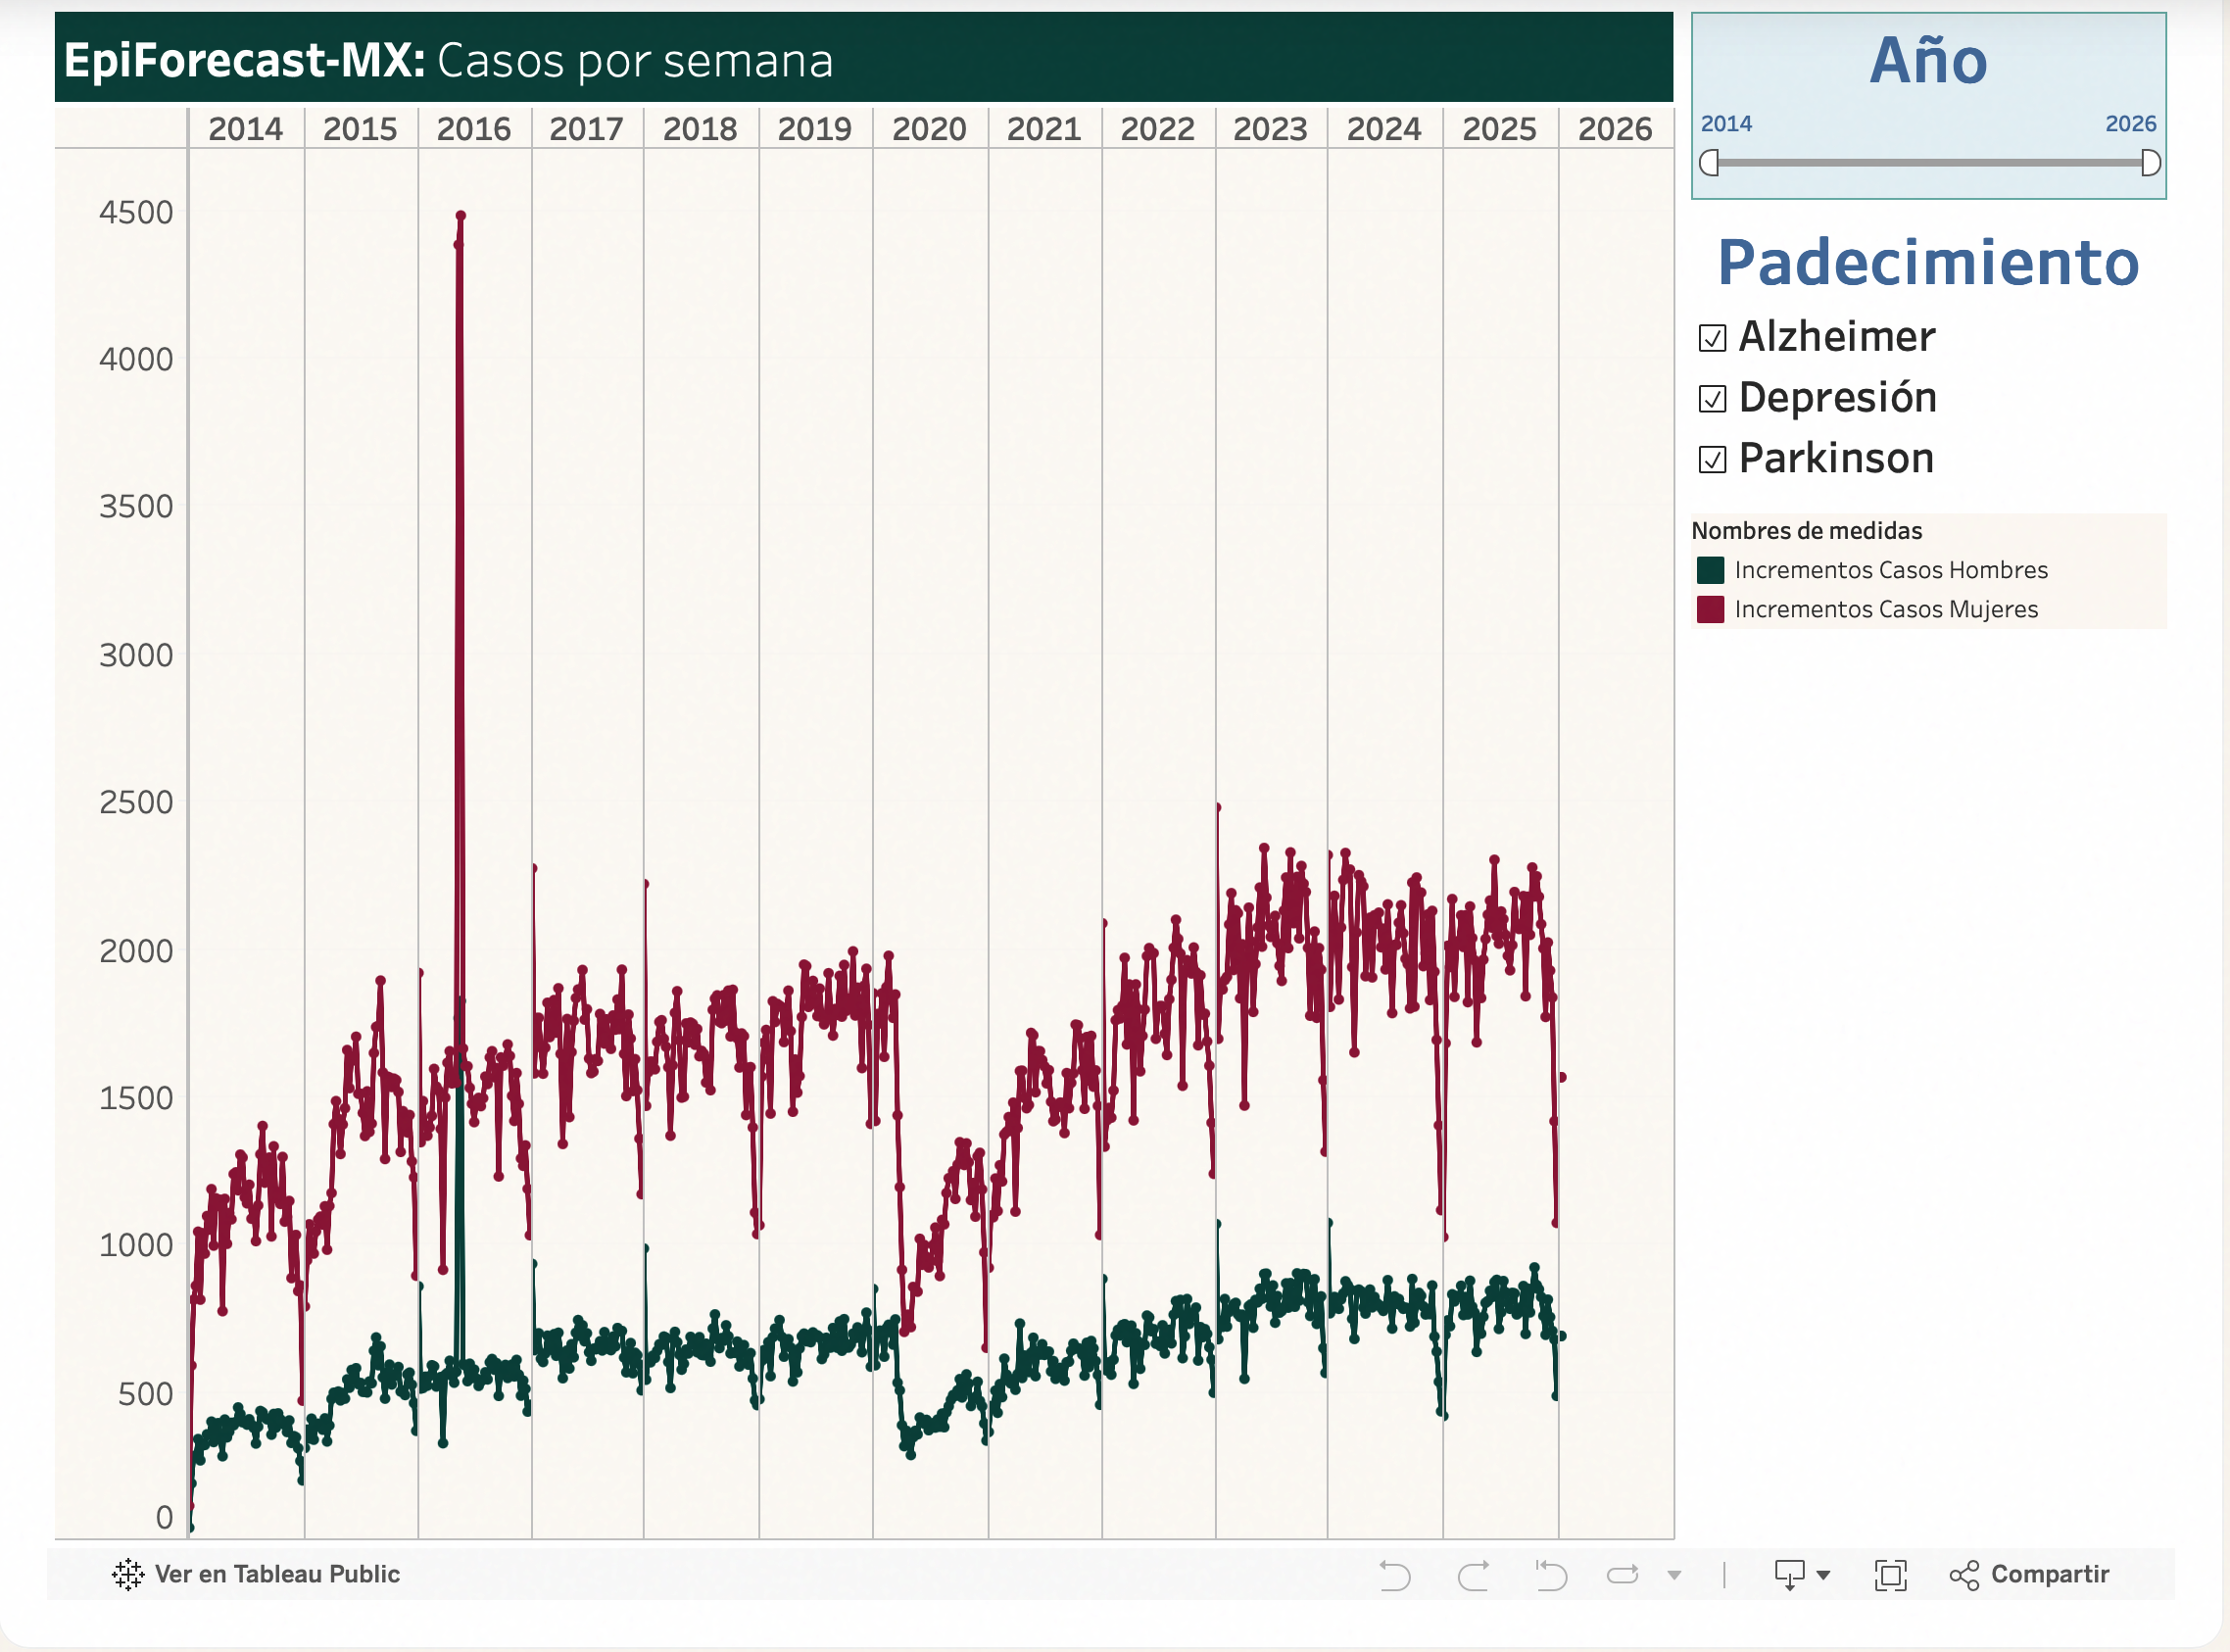
\includegraphics[width=\textwidth]{img/tableau_casos_semanales.png}
    \caption{Incremento de casos semanales por sexo.}
\end{figure}

\subsection{Predicciones epidemiológicas}

\textbf{Nota:} las predicciones mostradas son simuladas en esta etapa.

Esta visualización combina los incrementos históricos de casos anuales por sexo con la predicción generada por el modelo seleccionado para cada padecimiento. Su propósito es exploratorio y demostrativo, y servirá como base para integrar predicciones validadas en entregas posteriores.

\begin{figure}[H]
    \centering
    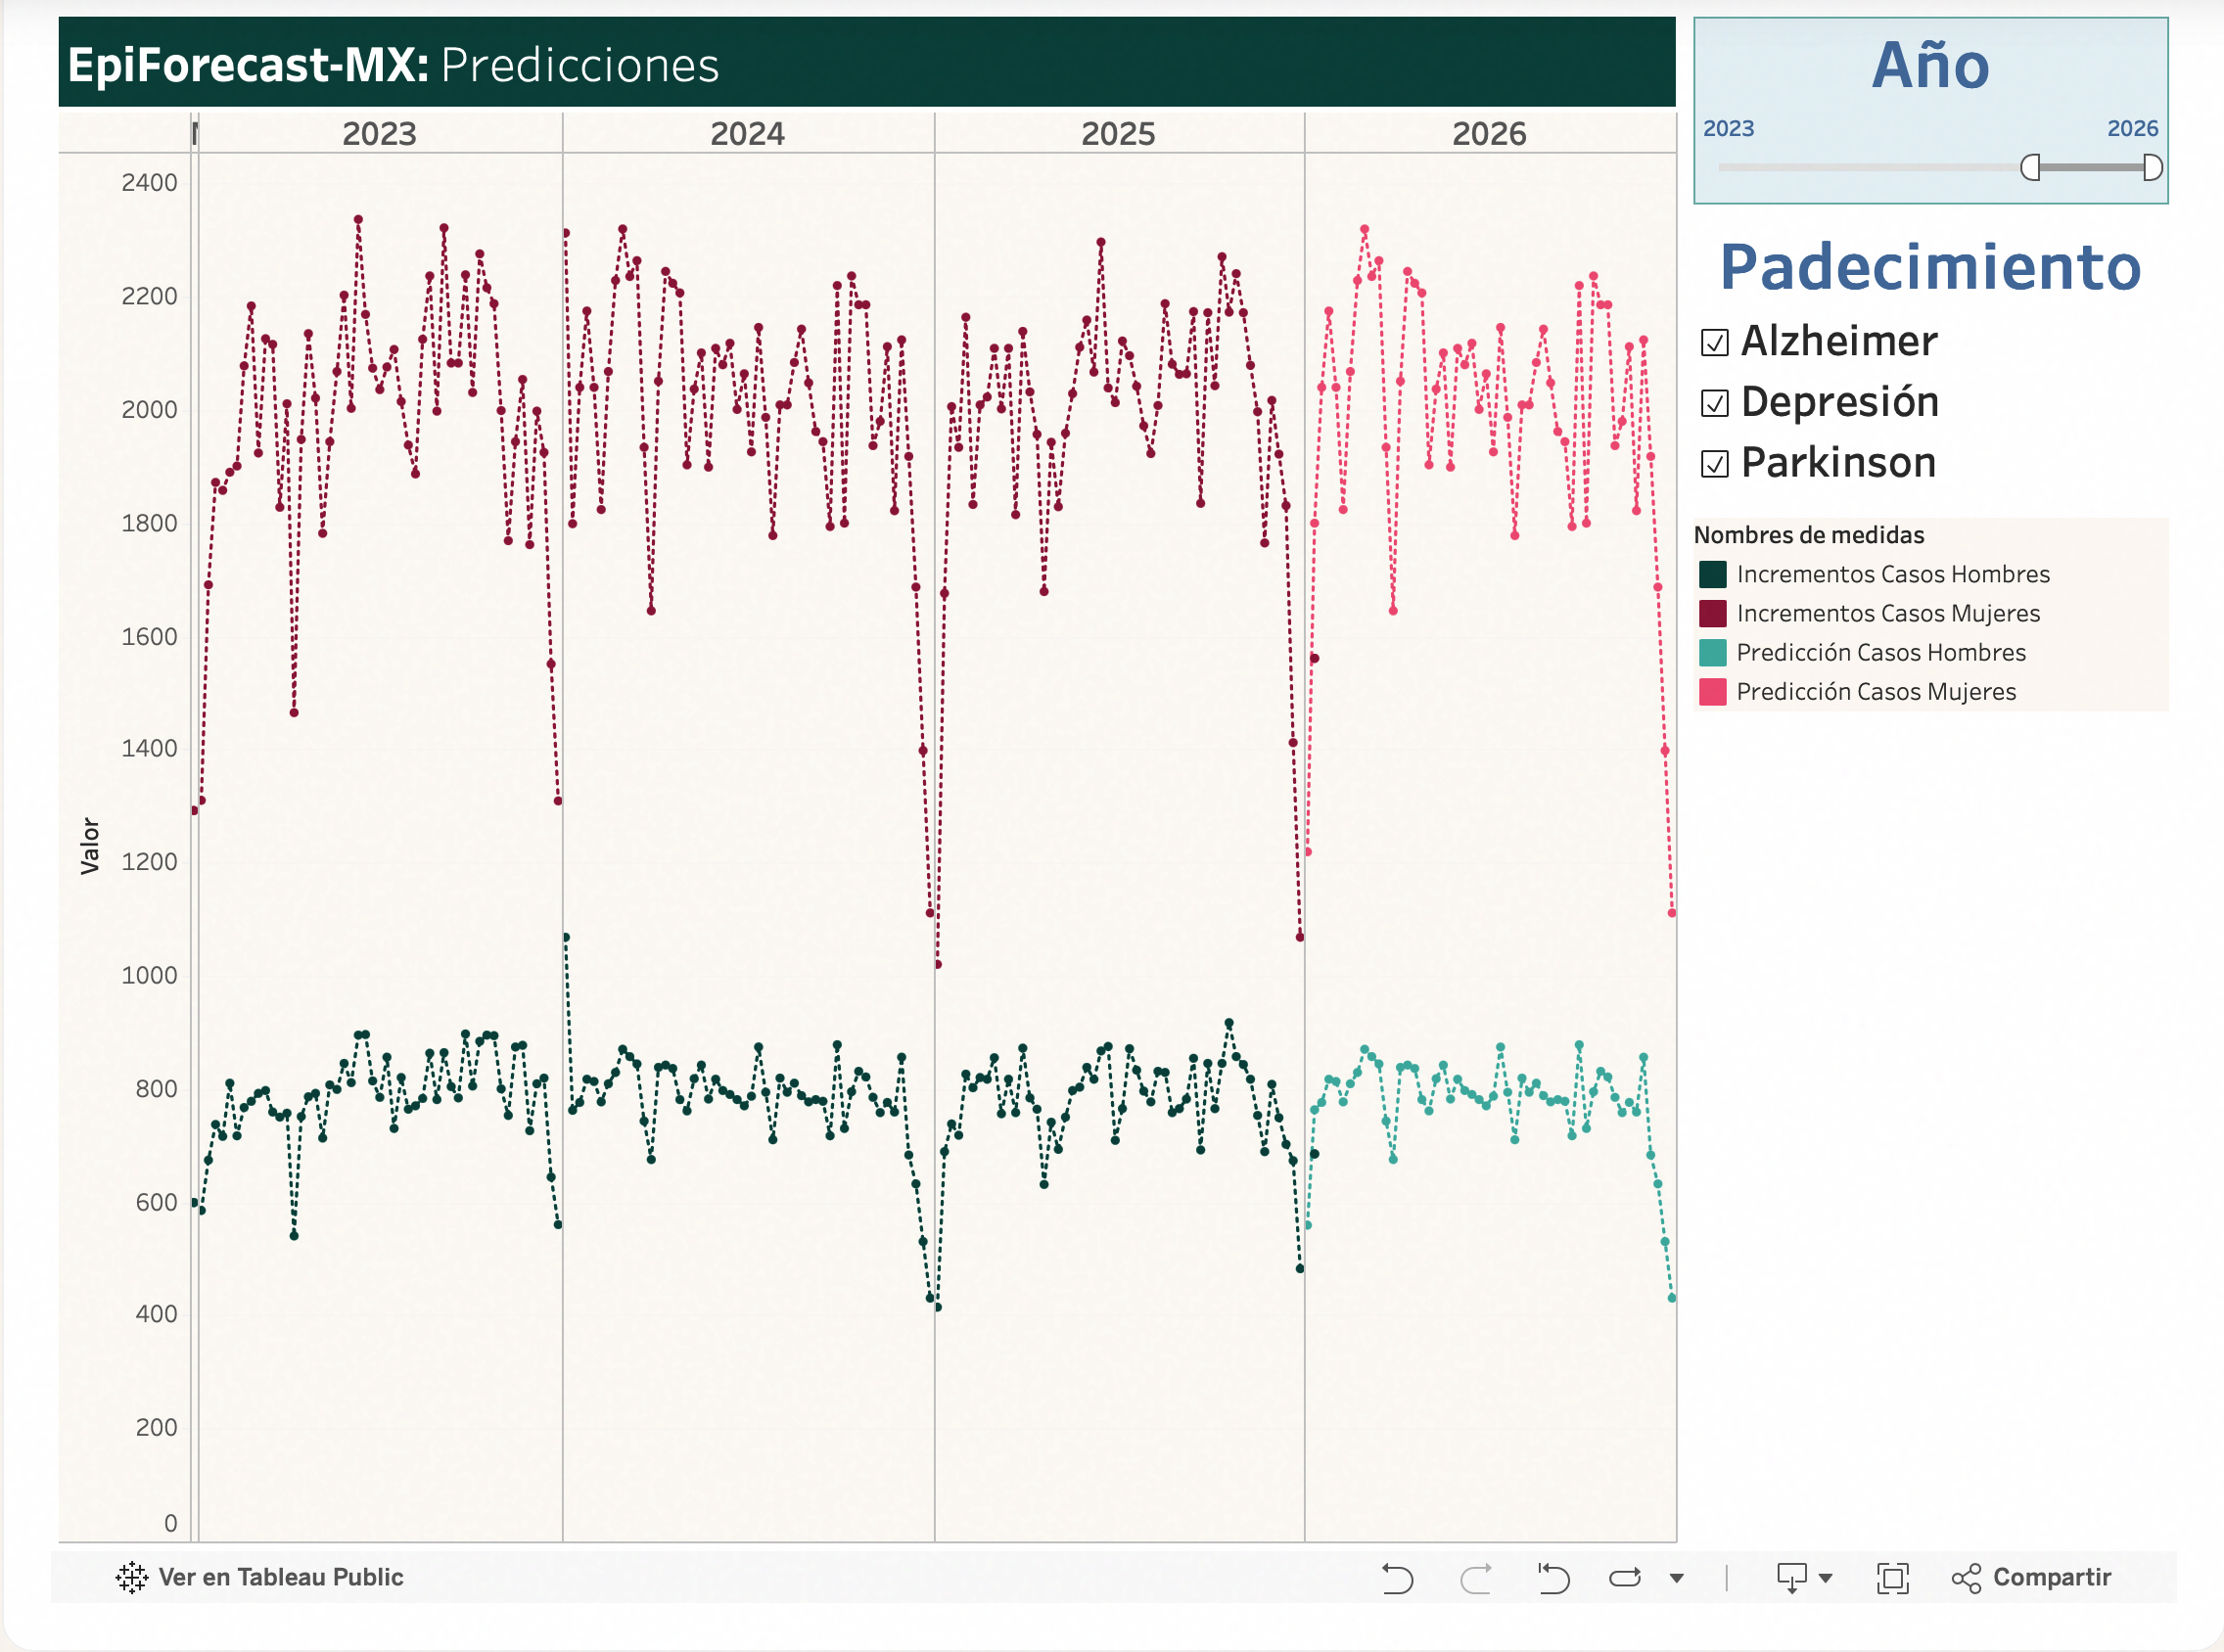
\includegraphics[width=\textwidth]{img/tableau_predicciones.png}
    \caption{Predicciones epidemiológicas (simuladas).}
\end{figure}

\newpage

% ============================================================
% SECCIÓN 9
% ============================================================
\section{Síntesis del Avance: Ingeniería de Características y Visualización}

El trabajo desarrollado en esta etapa corresponde al \textbf{Avance 2: Ingeniería de Características}, y se enfoca en enriquecer estructuralmente el dataset epidemiológico mediante la integración de información demográfica y territorial proveniente de INEGI, así como en formalizar una primera capa de visualización interactiva del proyecto \textbf{EpiForecast-MX}.

\subsection{Pipeline de Datos y Enriquecimiento}

El pipeline general del proyecto se mantiene intacto y versionado en el repositorio. Sobre este pipeline se añadió una rama específica de ingeniería de características, cuyas etapas principales son:

\begin{enumerate}
    \item \textbf{Consumo del dataset epidemiológico limpio:} Se parte del archivo \code{data\_prepare\_\allowbreak <tipo>.csv}, resultado directo del pipeline de limpieza y transformación del SINAVE.
    \item \textbf{Extracción de datos INEGI:} Descarga programática de información poblacional y territorial desde la API PxWeb de INEGI, utilizando como referencia el Censo de Población y Vivienda 2020.
    \item \textbf{Construcción del dataset demográfico base:} Población total, población por sexo, superficie territorial por entidad y validación interna (Hombres + Mujeres = Total).
    \item \textbf{Ingeniería de características territoriales y demográficas:} Generación de variables continuas y categóricas (densidad poblacional, tamaño poblacional, extensión territorial, ratio H/M, región socio-territorial).
    \item \textbf{Normalización y merge por entidad federativa:} Replicando la lógica del módulo \code{MapeaInegi}, se normalizan nombres de entidades y se realiza un \textit{left join} entre el boletín epidemiológico y el dataset INEGI.
    \item \textbf{Salida dual del pipeline:} CSV versionado para análisis y modelado, y archivo Excel como insumo para Tableau.
\end{enumerate}

\subsection{Hallazgos Clave de la Ingeniería de Características}

\paragraph{Estructura territorial y demográfica.}
La densidad poblacional emerge como una de las variables más discriminantes entre entidades. Las clasificaciones por percentiles generan grupos balanceados, útiles para análisis comparativos. La mayoría de las entidades presentan un ratio hombres/mujeres cercano a 1.

\paragraph{Integración con epidemiología.}
El merge con INEGI no introduce pérdida de registros, confirmando consistencia en la variable entidad. Las nuevas categorías permiten analizar patrones epidemiológicos desde una perspectiva estructural, no solo temporal. La segmentación territorial revela heterogeneidades que no son visibles en agregados nacionales simples.

\subsection{Contribución al Modelado Futuro}

\begin{enumerate}
    \item \textbf{Variables estructurales listas para usar:} Las categorías territoriales y demográficas pueden emplearse como variables exógenas, estratos de análisis o criterios de segmentación.
    \item \textbf{Reducción de sesgos por escala:} Normalizar por población y densidad evita conclusiones dominadas por entidades grandes.
    \item \textbf{Mejor interpretabilidad:} Las variables categóricas derivadas permiten explicar resultados a audiencias no técnicas.
    \item \textbf{Compatibilidad con modelos temporales:} El dataset enriquecido conserva la estructura temporal necesaria para Prophet, ARIMA o modelos híbridos.
\end{enumerate}

\subsection{Limitaciones de esta Etapa}

La regionalización de salud mental es una asignación estructural inicial, no completamente \textit{data-driven}. La información demográfica es estática (Censo 2020) y no captura cambios poblacionales anuales. Las visualizaciones en Tableau Public no están conectadas a una fuente dinámica. Las predicciones mostradas son simuladas y no deben interpretarse como resultados finales.

\newpage

% ============================================================
% CONCLUSIONES FINALES DEL EQUIPO
% ============================================================
\section*{Conclusiones Finales del Equipo}
\addcontentsline{toc}{section}{Conclusiones Finales del Equipo}

El desarrollo del Avance 2 consolida la transición del proyecto \textbf{EpiForecast-MX} desde la limpieza y exploración inicial de datos hacia una fase de preparación estructurada y orientada al modelado predictivo. A continuación se presentan las conclusiones colectivas del equipo respecto a esta etapa.

\paragraph{Enriquecimiento con impacto analítico real.}
La integración de variables demográficas y territoriales de INEGI no fue un ejercicio meramente acumulativo: cada variable añadida responde a una hipótesis sobre los determinantes estructurales de la incidencia epidemiológica en México. La densidad poblacional, la regionalización socio-urbana y el tamaño poblacional por rangos fijos demostraron ser las características con mayor potencial discriminante para estratificar patrones entre entidades federativas. Este enriquecimiento transforma el dataset de una colección de series temporales aisladas en un recurso multidimensional con contexto territorial.

\paragraph{Pipeline reproducible como activo del proyecto.}
El diseño modular del pipeline, desde la extracción automatizada de boletines hasta la generación del dataset enriquecido con salida dual (CSV y Excel), garantiza que cualquier miembro del equipo o evaluador pueda replicar íntegramente los resultados. La combinación de DVC para versionado de datos, GitHub Actions para automatización y scripts parametrizados refuerza el compromiso del equipo con las mejores prácticas de MLOps y con el marco metodológico CRISP-ML(Q).

\paragraph{Visualización como instrumento de validación y comunicación.}
Las visualizaciones desarrolladas, tanto en Python como en Tableau, cumplieron una doble función: sirvieron como herramienta de validación interna para detectar inconsistencias o confirmar patrones esperados, y como medio de comunicación hacia los stakeholders del IMSS. La segmentación por categorías territoriales en las series de tiempo reveló heterogeneidades regionales que permanecen ocultas en los agregados nacionales, reforzando la pertinencia de un enfoque desagregado para el pronóstico.

\paragraph{Base sólida para la fase de modelado.}
El dataset resultante de esta etapa está preparado para alimentar directamente los modelos de pronóstico planificados. Las variables categóricas derivadas podrán utilizarse como regresores exógenos en Prophet o como criterios de segmentación para entrenar modelos diferenciados por región o condición. La normalización por población y densidad mitiga sesgos de escala que, de no tratarse, distorsionarían las predicciones en favor de las entidades más pobladas.

\paragraph{Trabajo colaborativo y aprendizaje continuo.}
Esta entrega reflejó una dinámica de trabajo donde cada integrante aportó desde su experiencia profesional: la perspectiva de infraestructura de datos del IMSS, la visión de ingeniería de sistemas y la experiencia en operaciones de datos se integraron de forma orgánica. El equipo identificó también áreas de mejora, como la necesidad de una regionalización más robusta basada en datos y la incorporación de fuentes dinámicas para actualizar las variables demográficas más allá del Censo 2020.

\paragraph{Próximos pasos.}
Con la ingeniería de características consolidada, el equipo se enfocará en la selección final de variables, la implementación de modelos de pronóstico basados en Prophet con regresores exógenos, y la evaluación de desempeño mediante intervalos de predicción. El objetivo inmediato es cerrar la brecha entre un dataset bien preparado y un sistema de pronóstico funcional que aporte valor estratégico al IMSS para la planificación de recursos en salud mental y neurología a nivel nacional y subnacional.

\newpage

% ============================================================
% REFLEXIONES DEL EQUIPO
% ============================================================
\section*{Reflexiones del Equipo}
\addcontentsline{toc}{section}{Reflexiones del Equipo}

\begin{wrapfigure}{l}{3.5cm}
    \vspace{-0.4cm}
    \centering
    \includegraphics[width=3.2cm, height=3.2cm, keepaspectratio]{JARCOS3.png}
    \vspace{-0.4cm}
\end{wrapfigure}
\textbf{Juan Carlos Pérez} --- \textit{``Desde el enfoque de datos, este avance marcó un punto de consolidación del proyecto. El pipeline permitió pasar de un dataset corregido a uno estructuralmente enriquecido, manteniendo consistencia, reproducibilidad y control sobre cada transformación. La ingeniería de características obligó a evaluar cuidadosamente qué variables realmente aportaban información y cuáles solo agregaban complejidad innecesaria. El uso de visualizaciones y series de tiempo fue clave para validar decisiones del pipeline, ya que permitió confirmar visualmente patrones, tendencias y posibles errores. Este avance reforzó la idea de que un pipeline sólido no solo prepara datos para modelar, sino que también funciona como una herramienta de validación continua del análisis.''}

\vspace{1em}

\begin{wrapfigure}{l}{3.5cm}
    \vspace{-0.4cm}
    \centering
    
\includegraphics[width=3.2cm, height=3.2cm, keepaspectratio]{JARS3.png}
    \vspace{-0.4cm}
\end{wrapfigure}
\textbf{Javier Rebull} --- \textit{``Pienso que el principal aprendizaje de esta entrega fue pensar el proyecto como un sistema vivo y no como un análisis estático. El diseño del pipeline y de los scripts considera explícitamente la detección de nuevos boletines epidemiológicos y la actualización progresiva del dataset, reduciendo la dependencia de procesos manuales. Este enfoque facilita la escalabilidad del proyecto y garantiza que los resultados puedan mantenerse actualizados conforme se publique nueva información oficial. El trabajo realizado deja sentadas las bases para que el proyecto evolucione hacia un flujo completamente automatizado, alineado con buenas prácticas de ingeniería de datos y operación continua.''}

\vspace{1em}

\begin{wrapfigure}{l}{3.5cm}
    \vspace{-0.4cm}
    \centering
    
\includegraphics[width=3.2cm, height=3.2cm, keepaspectratio]{Luis3.png}
    \vspace{-0.4cm}
\end{wrapfigure}
\textbf{Luis Sánchez} --- \textit{``Desde el punto de vista de la extracción y uso de datos de INEGI, este avance permitió integrar información demográfica y territorial de manera coherente con los datos epidemiológicos. La construcción de categorías, tanto continuas como discretizadas, ayudó a traducir variables complejas en indicadores interpretables y comparables. Asimismo, el trabajo en visualización, particularmente mediante Tableau, evidenció la importancia de contar con una capa clara de comunicación que permita explorar los datos sin perder rigor analítico. Este avance mostró que la correcta clasificación de variables y su representación visual son fundamentales para revelar patrones regionales y demográficos que no son evidentes en tablas o estadísticas agregadas y que nos permitirán llevar la predicción al siguiente nivel en etapas posteriores de modelado.''}

\newpage

% ============================================================
% REFERENCIAS
% ============================================================
\section*{Referencias}
\addcontentsline{toc}{section}{Referencias}

\begin{small}
\begin{enumerate}[leftmargin=*]
    \item Alegría, M., et al. (2018). \textit{Social determinants of mental health}. Social Psychiatry and Psychiatric Epidemiology.
    \item Brownlee, J. (2020). \textit{How to Choose a Feature Selection Method for Machine Learning}. Machine Learning Mastery.
    \item CONAPO (2020). \textit{Índices de marginación por entidad federativa y municipio}. Consejo Nacional de Población.
    \item CONEVAL (2020). \textit{Índices de marginación por entidad federativa y municipio}.
    \item Costa, R. (2022). \textit{The CRISP-ML Methodology: A Step-by-Step Approach to Real-World Machine Learning Projects}.
    \item Elliott, P., \& Wartenberg, D. (2004). \textit{Spatial epidemiology}. Environmental Health Perspectives, 112(9).
    \item Galli, S. (2022). \textit{Python Feature Engineering Cookbook} (2.ª ed.). Packt Publishing.
    \item Hernández-Sampieri, R., \& Mendoza, C. (2023). \textit{Metodología de la investigación: Las rutas de la investigación cuantitativa, cualitativa y mixta} (3.ª ed.). McGraw-Hill.
    \item Huang, C. Y., \& Dai, H. L. (2021). \textit{Learning from class-imbalanced data}. Data Science in Finance and Economics, 1(1).
    \item INEGI (s. f.). \textit{Áreas geográficas e indicadores territoriales}. Instituto Nacional de Estadística y Geografía.
    \item INEGI (s. f.). \textit{Localidades urbanas y rurales en México}. INEGI.
    \item INEGI (s. f.). \textit{Marco geoestadístico y datos poblacionales}. INEGI.
    \item INEGI (2024). \textit{PxWeb API: Población por entidad federativa y sexo}. INEGI.
    \item Kumar Mukhiya, S., \& Ahmed, U. (2020). \textit{Hands-On Exploratory Data Analysis with Python}. Packt Publishing.
    \item Organización Panamericana de la Salud (2021). \textit{La salud mental en la región de las Américas}. OPS.
    \item Organización Mundial de la Salud (2014). \textit{Social determinants of mental health}. WHO.
    \item Organización Mundial de la Salud (2022). \textit{World mental health report: Transforming mental health for all}. WHO.
    \item Organización Mundial de la Salud (2025). \textit{ICD-11 2025 update}. WHO.
    \item Pérez-Hernández, R. \textit{Enfermedades neurológicas y trastornos mentales en México 2014--2024}.
    \item Secretaría de Salud (s. f.). \textit{Boletín Epidemiológico: SINAVE}. Gobierno de México.
    \item Secretaría de Salud (s. f.). \textit{Directorio de unidades de atención en salud mental}. Gobierno de México.
    \item SINAVE (s. f.). \textit{Sistema Nacional de Vigilancia Epidemiológica}. Secretaría de Salud.
    \item Visengeriyeva, L., et al. (2023). \textit{CRISP-ML(Q): The ML Lifecycle Process}. INNOQ / MLOps.
\end{enumerate}
\end{small}

\end{document}
